\documentclass[twoside]{book}

% Packages required by doxygen
\usepackage{fixltx2e}
\usepackage{calc}
\usepackage{doxygen}
\usepackage[export]{adjustbox} % also loads graphicx
\usepackage{graphicx}
\usepackage[utf8]{inputenc}
\usepackage{makeidx}
\usepackage{multicol}
\usepackage{multirow}
\PassOptionsToPackage{warn}{textcomp}
\usepackage{textcomp}
\usepackage[nointegrals]{wasysym}
\usepackage[table]{xcolor}

% Font selection
\usepackage[T1]{fontenc}
\usepackage[scaled=.90]{helvet}
\usepackage{courier}
\usepackage{amssymb}
\usepackage{sectsty}
\renewcommand{\familydefault}{\sfdefault}
\allsectionsfont{%
  \fontseries{bc}\selectfont%
  \color{darkgray}%
}
\renewcommand{\DoxyLabelFont}{%
  \fontseries{bc}\selectfont%
  \color{darkgray}%
}
\newcommand{\+}{\discretionary{\mbox{\scriptsize$\hookleftarrow$}}{}{}}

% Page & text layout
\usepackage{geometry}
\geometry{%
  a4paper,%
  top=2.5cm,%
  bottom=2.5cm,%
  left=2.5cm,%
  right=2.5cm%
}
\tolerance=750
\hfuzz=15pt
\hbadness=750
\setlength{\emergencystretch}{15pt}
\setlength{\parindent}{0cm}
\setlength{\parskip}{0.2cm}
\makeatletter
\renewcommand{\paragraph}{%
  \@startsection{paragraph}{4}{0ex}{-1.0ex}{1.0ex}{%
    \normalfont\normalsize\bfseries\SS@parafont%
  }%
}
\renewcommand{\subparagraph}{%
  \@startsection{subparagraph}{5}{0ex}{-1.0ex}{1.0ex}{%
    \normalfont\normalsize\bfseries\SS@subparafont%
  }%
}
\makeatother

% Headers & footers
\usepackage{fancyhdr}
\pagestyle{fancyplain}
\fancyhead[LE]{\fancyplain{}{\bfseries\thepage}}
\fancyhead[CE]{\fancyplain{}{}}
\fancyhead[RE]{\fancyplain{}{\bfseries\leftmark}}
\fancyhead[LO]{\fancyplain{}{\bfseries\rightmark}}
\fancyhead[CO]{\fancyplain{}{}}
\fancyhead[RO]{\fancyplain{}{\bfseries\thepage}}
\fancyfoot[LE]{\fancyplain{}{}}
\fancyfoot[CE]{\fancyplain{}{}}
\fancyfoot[RE]{\fancyplain{}{\bfseries\scriptsize Generated on Thu Apr 30 2015 15\+:32\+:21 for True\+North Time\+Warp Benchmark by Doxygen }}
\fancyfoot[LO]{\fancyplain{}{\bfseries\scriptsize Generated on Thu Apr 30 2015 15\+:32\+:21 for True\+North Time\+Warp Benchmark by Doxygen }}
\fancyfoot[CO]{\fancyplain{}{}}
\fancyfoot[RO]{\fancyplain{}{}}
\renewcommand{\footrulewidth}{0.4pt}
\renewcommand{\chaptermark}[1]{%
  \markboth{#1}{}%
}
\renewcommand{\sectionmark}[1]{%
  \markright{\thesection\ #1}%
}

% Indices & bibliography
\usepackage{natbib}
\usepackage[titles]{tocloft}
\setcounter{tocdepth}{3}
\setcounter{secnumdepth}{5}
\makeindex

% Hyperlinks (required, but should be loaded last)
\usepackage{ifpdf}
\ifpdf
  \usepackage[pdftex,pagebackref=true]{hyperref}
\else
  \usepackage[ps2pdf,pagebackref=true]{hyperref}
\fi
\hypersetup{%
  colorlinks=true,%
  linkcolor=blue,%
  citecolor=blue,%
  unicode%
}

% Custom commands
\newcommand{\clearemptydoublepage}{%
  \newpage{\pagestyle{empty}\cleardoublepage}%
}


%===== C O N T E N T S =====

\begin{document}

% Titlepage & ToC
\hypersetup{pageanchor=false,
             bookmarks=true,
             bookmarksnumbered=true,
             pdfencoding=unicode
            }
\pagenumbering{roman}
\begin{titlepage}
\vspace*{7cm}
\begin{center}%
{\Large True\+North Time\+Warp Benchmark }\\
\vspace*{1cm}
{\large Generated by Doxygen 1.8.9.1}\\
\vspace*{0.5cm}
{\small Thu Apr 30 2015 15:32:21}\\
\end{center}
\end{titlepage}
\clearemptydoublepage
\tableofcontents
\clearemptydoublepage
\pagenumbering{arabic}
\hypersetup{pageanchor=true}

%--- Begin generated contents ---
\chapter{True North Timewarp Benchmark Simulation}
\label{index}\hypertarget{index}{}This is the T\+N\+T Benchmarking sim. 
\chapter{Data Structure Index}
\section{Data Structures}
Here are the data structures with brief descriptions\+:\begin{DoxyCompactList}
\item\contentsline{section}{\hyperlink{structaxon_state}{axon\+State} }{\pageref{structaxon_state}}{}
\item\contentsline{section}{\hyperlink{structinput_simulator_state}{input\+Simulator\+State} \\*Struct that manages the spike generator }{\pageref{structinput_simulator_state}}{}
\item\contentsline{section}{\hyperlink{structleak_fun_del}{leak\+Fun\+Del} \\*This is a dec }{\pageref{structleak_fun_del}}{}
\item\contentsline{section}{\hyperlink{struct_msg___data}{Msg\+\_\+\+Data} \\*Main message struct }{\pageref{struct_msg___data}}{}
\item\contentsline{section}{\hyperlink{struct_neuron_model}{Neuron\+Model} \\*This struct maintains the state of an individual neuron.\+The neuron struct contains the parameters needed to maintain state in the neuron, along with references to output commands (dendrites) }{\pageref{struct_neuron_model}}{}
\item\contentsline{section}{\hyperlink{structneuron_state}{neuron\+State} }{\pageref{structneuron_state}}{}
\item\contentsline{section}{\hyperlink{structrandom_spikes}{random\+Spikes} \\*Struct that genreates spikes randomly }{\pageref{structrandom_spikes}}{}
\item\contentsline{section}{\hyperlink{unionreset_rate}{reset\+Rate} \\*Reset\+Rate This is a support union for neuron reset rates }{\pageref{unionreset_rate}}{}
\item\contentsline{section}{\hyperlink{structreverse_leak_del}{reverse\+Leak\+Del} \\*This fun }{\pageref{structreverse_leak_del}}{}
\item\contentsline{section}{\hyperlink{structselected_spikes}{selected\+Spikes} }{\pageref{structselected_spikes}}{}
\item\contentsline{section}{\hyperlink{structsynapse_state}{synapse\+State} \\*Synapse state structure }{\pageref{structsynapse_state}}{}
\end{DoxyCompactList}

\chapter{File Index}
\section{File List}
Here is a list of all files with brief descriptions\+:\begin{DoxyCompactList}
\item\contentsline{section}{/\+Users/\+Mark/\+Development/\+True\+North/tnt\+\_\+benchmark/\hyperlink{assist_8c}{assist.\+c} }{\pageref{assist_8c}}{}
\item\contentsline{section}{/\+Users/\+Mark/\+Development/\+True\+North/tnt\+\_\+benchmark/\hyperlink{assist_8h}{assist.\+h} }{\pageref{assist_8h}}{}
\item\contentsline{section}{/\+Users/\+Mark/\+Development/\+True\+North/tnt\+\_\+benchmark/\hyperlink{mappings_8c}{mappings.\+c} }{\pageref{mappings_8c}}{}
\item\contentsline{section}{/\+Users/\+Mark/\+Development/\+True\+North/tnt\+\_\+benchmark/\hyperlink{model__main_8c}{model\+\_\+main.\+c} }{\pageref{model__main_8c}}{}
\item\contentsline{section}{/\+Users/\+Mark/\+Development/\+True\+North/tnt\+\_\+benchmark/\hyperlink{model__main_8h}{model\+\_\+main.\+h} }{\pageref{model__main_8h}}{}
\item\contentsline{section}{/\+Users/\+Mark/\+Development/\+True\+North/tnt\+\_\+benchmark/\hyperlink{spike__generator_8c}{spike\+\_\+generator.\+c} }{\pageref{spike__generator_8c}}{}
\item\contentsline{section}{/\+Users/\+Mark/\+Development/\+True\+North/tnt\+\_\+benchmark/\hyperlink{spike__generator_8h}{spike\+\_\+generator.\+h} \\*Spike\+\_\+generate defines a L\+P state and functions that generate output at a tuneable rate }{\pageref{spike__generator_8h}}{}
\item\contentsline{section}{\hyperlink{mapping__specifications_8rtf}{mapping\+\_\+specifications.\+rtf} }{\pageref{mapping__specifications_8rtf}}{}
\item\contentsline{section}{/\+Users/\+Mark/\+Development/\+True\+North/tnt\+\_\+benchmark/models/\hyperlink{neuron__model_8c}{neuron\+\_\+model.\+c} }{\pageref{neuron__model_8c}}{}
\item\contentsline{section}{/\+Users/\+Mark/\+Development/\+True\+North/tnt\+\_\+benchmark/models/\hyperlink{neuron__model_8h}{neuron\+\_\+model.\+h} }{\pageref{neuron__model_8h}}{}
\item\contentsline{section}{/\+Users/\+Mark/\+Development/\+True\+North/tnt\+\_\+benchmark/models/\hyperlink{synapse_8h}{synapse.\+h} }{\pageref{synapse_8h}}{}
\end{DoxyCompactList}

\chapter{Data Structure Documentation}
\hypertarget{structleak_fun_del}{}\section{leak\+Fun\+Del Struct Reference}
\label{structleak_fun_del}\index{leak\+Fun\+Del@{leak\+Fun\+Del}}


This is a dec.  




{\ttfamily \#include $<$neuron.\+h$>$}



\subsection{Detailed Description}
This is a dec. 

of a function that allows for neurons to have different leak functions. At this point, the only function is a dummy one. The functions alter the neuron\textquotesingle{}s current voltage. 

The documentation for this struct was generated from the following file\+:\begin{DoxyCompactItemize}
\item 
/home/mplagge/development/tnt\+\_\+benchmark/models/\hyperlink{neuron_8h}{neuron.\+h}\end{DoxyCompactItemize}

\hypertarget{struct_msg___data}{}\section{Msg\+\_\+\+Data Struct Reference}
\label{struct_msg___data}\index{Msg\+\_\+\+Data@{Msg\+\_\+\+Data}}


{\ttfamily \#include $<$assist.\+h$>$}

\subsection*{Data Fields}
\begin{DoxyCompactItemize}
\item 
tw\+\_\+lpid \hyperlink{struct_msg___data_ac94c7cb1b3f009936733d0f0cec9f72a}{sender}
\item 
\hyperlink{mappings_8c_adc0d1d400308f82e4d42245c2fd946b9}{\+\_\+id\+Type} \hyperlink{struct_msg___data_af4e0329991e30bd3958b93c3bbb3038d}{sender\+Local\+I\+D}
\item 
\hyperlink{mappings_8c_adc0d1d400308f82e4d42245c2fd946b9}{\+\_\+id\+Type} \hyperlink{struct_msg___data_a0ce9b87ee4780bfc676814cf8d485a97}{dest\+Core}
\item 
\hyperlink{mappings_8c_adc0d1d400308f82e4d42245c2fd946b9}{\+\_\+id\+Type} \hyperlink{struct_msg___data_aa0359599db6f5e6c68ac2b7123b4147a}{dest\+Local\+I\+D}
\item 
\hyperlink{mappings_8c_adc0d1d400308f82e4d42245c2fd946b9}{\+\_\+id\+Type} \hyperlink{struct_msg___data_a13b05c6b2a199a7bdf79a18b9e7c22e9}{source\+Core}
\item 
enum \hyperlink{assist_8h_ad29858f6d8ab73f2970f41cb21a76b84}{events} \hyperlink{struct_msg___data_ab8720847cee557678e9bfc7da95d46bf}{type}
\item 
\hyperlink{mappings_8c_a368ddcd71f7b61cb0f918f22d07ce999}{\+\_\+ne\+Volt\+Type} \hyperlink{struct_msg___data_a20818fc301603eac9d3685ba53424699}{prev\+Voltage}
\begin{DoxyCompactList}\small\item\em This saves the old state of the neuron, before firing, so that roll back functions will occur. \end{DoxyCompactList}\end{DoxyCompactItemize}


\subsection{Detailed Description}


Definition at line 137 of file assist.\+h.



\subsection{Field Documentation}
\hypertarget{struct_msg___data_a0ce9b87ee4780bfc676814cf8d485a97}{}\index{Msg\+\_\+\+Data@{Msg\+\_\+\+Data}!dest\+Core@{dest\+Core}}
\index{dest\+Core@{dest\+Core}!Msg\+\_\+\+Data@{Msg\+\_\+\+Data}}
\subsubsection[{dest\+Core}]{\setlength{\rightskip}{0pt plus 5cm}{\bf \+\_\+id\+Type} dest\+Core}\label{struct_msg___data_a0ce9b87ee4780bfc676814cf8d485a97}


Definition at line 140 of file assist.\+h.

\hypertarget{struct_msg___data_aa0359599db6f5e6c68ac2b7123b4147a}{}\index{Msg\+\_\+\+Data@{Msg\+\_\+\+Data}!dest\+Local\+I\+D@{dest\+Local\+I\+D}}
\index{dest\+Local\+I\+D@{dest\+Local\+I\+D}!Msg\+\_\+\+Data@{Msg\+\_\+\+Data}}
\subsubsection[{dest\+Local\+I\+D}]{\setlength{\rightskip}{0pt plus 5cm}{\bf \+\_\+id\+Type} dest\+Local\+I\+D}\label{struct_msg___data_aa0359599db6f5e6c68ac2b7123b4147a}


Definition at line 141 of file assist.\+h.

\hypertarget{struct_msg___data_a20818fc301603eac9d3685ba53424699}{}\index{Msg\+\_\+\+Data@{Msg\+\_\+\+Data}!prev\+Voltage@{prev\+Voltage}}
\index{prev\+Voltage@{prev\+Voltage}!Msg\+\_\+\+Data@{Msg\+\_\+\+Data}}
\subsubsection[{prev\+Voltage}]{\setlength{\rightskip}{0pt plus 5cm}{\bf \+\_\+ne\+Volt\+Type} prev\+Voltage}\label{struct_msg___data_a20818fc301603eac9d3685ba53424699}


This saves the old state of the neuron, before firing, so that roll back functions will occur. 



Definition at line 145 of file assist.\+h.



Referenced by neuron\+Receive\+Message().

\hypertarget{struct_msg___data_ac94c7cb1b3f009936733d0f0cec9f72a}{}\index{Msg\+\_\+\+Data@{Msg\+\_\+\+Data}!sender@{sender}}
\index{sender@{sender}!Msg\+\_\+\+Data@{Msg\+\_\+\+Data}}
\subsubsection[{sender}]{\setlength{\rightskip}{0pt plus 5cm}tw\+\_\+lpid sender}\label{struct_msg___data_ac94c7cb1b3f009936733d0f0cec9f72a}


Definition at line 138 of file assist.\+h.

\hypertarget{struct_msg___data_af4e0329991e30bd3958b93c3bbb3038d}{}\index{Msg\+\_\+\+Data@{Msg\+\_\+\+Data}!sender\+Local\+I\+D@{sender\+Local\+I\+D}}
\index{sender\+Local\+I\+D@{sender\+Local\+I\+D}!Msg\+\_\+\+Data@{Msg\+\_\+\+Data}}
\subsubsection[{sender\+Local\+I\+D}]{\setlength{\rightskip}{0pt plus 5cm}{\bf \+\_\+id\+Type} sender\+Local\+I\+D}\label{struct_msg___data_af4e0329991e30bd3958b93c3bbb3038d}


Definition at line 139 of file assist.\+h.



Referenced by neuron\+Receive\+Message().

\hypertarget{struct_msg___data_a13b05c6b2a199a7bdf79a18b9e7c22e9}{}\index{Msg\+\_\+\+Data@{Msg\+\_\+\+Data}!source\+Core@{source\+Core}}
\index{source\+Core@{source\+Core}!Msg\+\_\+\+Data@{Msg\+\_\+\+Data}}
\subsubsection[{source\+Core}]{\setlength{\rightskip}{0pt plus 5cm}{\bf \+\_\+id\+Type} source\+Core}\label{struct_msg___data_a13b05c6b2a199a7bdf79a18b9e7c22e9}


Definition at line 142 of file assist.\+h.

\hypertarget{struct_msg___data_ab8720847cee557678e9bfc7da95d46bf}{}\index{Msg\+\_\+\+Data@{Msg\+\_\+\+Data}!type@{type}}
\index{type@{type}!Msg\+\_\+\+Data@{Msg\+\_\+\+Data}}
\subsubsection[{type}]{\setlength{\rightskip}{0pt plus 5cm}enum {\bf events} type}\label{struct_msg___data_ab8720847cee557678e9bfc7da95d46bf}


Definition at line 143 of file assist.\+h.



The documentation for this struct was generated from the following file\+:\begin{DoxyCompactItemize}
\item 
/\+Users/\+Mark/\+Development/\+True\+North/tnt\+\_\+benchmark/\hyperlink{assist_8h}{assist.\+h}\end{DoxyCompactItemize}

\hypertarget{struct_neuron_message}{}\section{Neuron\+Message Struct Reference}
\label{struct_neuron_message}\index{Neuron\+Message@{Neuron\+Message}}


{\ttfamily \#include $<$assist.\+h$>$}



\subsection{Detailed Description}


Definition at line 133 of file assist.\+h.



The documentation for this struct was generated from the following file\+:\begin{DoxyCompactItemize}
\item 
/\+Users/\+Mark/\+Development/\+True\+North/tnt\+\_\+benchmark/\hyperlink{assist_8h}{assist.\+h}\end{DoxyCompactItemize}

\hypertarget{struct_neuron_model}{}\section{Neuron\+Model Struct Reference}
\label{struct_neuron_model}\index{Neuron\+Model@{Neuron\+Model}}


This struct maintains the state of an individual neuron.\+The neuron struct contains the parameters needed to maintain state in the neuron, along with references to output commands (dendrites).  




{\ttfamily \#include $<$neuron.\+h$>$}



\subsection{Detailed Description}
This struct maintains the state of an individual neuron.\+The neuron struct contains the parameters needed to maintain state in the neuron, along with references to output commands (dendrites). 

Each parameter contained within {\bfseries [Cassidy2013]}\}{\bfseries [Preissl2012]}\}{\bfseries [Amir2013]}\}\textquotesingle{}s models of Neuromporphic design that operate with the neuron are contained within this struct. Consider this struct a proto-\/object, just sans functions. 

The documentation for this struct was generated from the following file\+:\begin{DoxyCompactItemize}
\item 
/home/mplagge/development/tnt\+\_\+benchmark/models/neuron.\+h\end{DoxyCompactItemize}

\hypertarget{structneuron_state}{}\section{neuron\+State Struct Reference}
\label{structneuron_state}\index{neuron\+State@{neuron\+State}}


{\ttfamily \#include $<$neuron.\+h$>$}



Collaboration diagram for neuron\+State\+:
\nopagebreak
\begin{figure}[H]
\begin{center}
\leavevmode
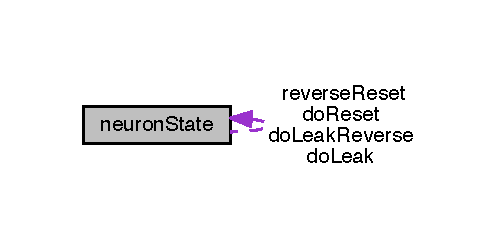
\includegraphics[width=239pt]{structneuron_state__coll__graph}
\end{center}
\end{figure}
\subsection*{Data Fields}
\begin{DoxyCompactItemize}
\item 
\hyperlink{assist_8h_a3f7a6e6a1210b6d9d7a42177dcb9634b}{\+\_\+id\+T} \hyperlink{structneuron_state_a76ef99e5766b6e36c3f41a2920e8c56c}{my\+Core\+I\+D}
\item 
\hyperlink{assist_8h_a3f7a6e6a1210b6d9d7a42177dcb9634b}{\+\_\+id\+T} \hyperlink{structneuron_state_ac24762c24aede292a2ce5df78114881c}{my\+Local\+I\+D}
\begin{DoxyCompactList}\small\item\em Neuron\textquotesingle{}s core\+I\+D. \end{DoxyCompactList}\item 
\hyperlink{assist_8h_abe1fc1b8f9efd1187e564bcb8de7f815}{\+\_\+volt\+T} \hyperlink{structneuron_state_a0fdd8f44c4105a94e17c4c58a51db486}{membrane\+Pot}
\begin{DoxyCompactList}\small\item\em Neuron\textquotesingle{}s local I\+D (from 0 -\/ j-\/1);. \end{DoxyCompactList}\item 
\hyperlink{assist_8h_abe1fc1b8f9efd1187e564bcb8de7f815}{\+\_\+volt\+T} \hyperlink{structneuron_state_ad17e1ac0b4bca75d10da8b0ab56edd6e}{prev\+Membrane\+Pot}
\begin{DoxyCompactList}\small\item\em current \char`\"{}voltage\char`\"{} of neuron \end{DoxyCompactList}\item 
\hyperlink{assist_8h_abe1fc1b8f9efd1187e564bcb8de7f815}{\+\_\+volt\+T} \hyperlink{structneuron_state_af321d0fa58028b78986160845189077e}{threshold}
\begin{DoxyCompactList}\small\item\em previous state membrane potential \end{DoxyCompactList}\item 
tw\+\_\+stime \hyperlink{structneuron_state_a0658ad1f8b57a00589c6ea84f9a4ab13}{last\+Active\+Time}
\begin{DoxyCompactList}\small\item\em neuron\textquotesingle{}s threshold value \end{DoxyCompactList}\item 
uint\+\_\+fast16\+\_\+t \hyperlink{structneuron_state_af8935bcba177f2f3dfb9119c39ef7dc5}{received\+Synapse\+Msgs}
\begin{DoxyCompactList}\small\item\em last time the neuron fired -\/ used for calculating leak and reverse functions. \end{DoxyCompactList}\item 
\hyperlink{neuron_8h_a48885ea6be5b55a2e24de9f97552d4ee}{neuron\+Fire\+Mode} \hyperlink{structneuron_state_a55890f9e021064df30e9d18a9df98845}{fire\+Mode}
\begin{DoxyCompactList}\small\item\em neuron firing parameters \end{DoxyCompactList}\item 
\hyperlink{neuron_8h_ae7e5990745cd949246894bfb633ca4a2}{reset\+Fun\+Del} \hyperlink{structneuron_state_afcf9d931e4fda519c43b4efeab687463}{do\+Reset}
\begin{DoxyCompactList}\small\item\em neuron\textquotesingle{}s firing mode \end{DoxyCompactList}\item 
\hyperlink{assist_8h_abe1fc1b8f9efd1187e564bcb8de7f815}{\+\_\+volt\+T} \hyperlink{structneuron_state_add87cc0b2bc3426f0fd870f7df6decd5}{reset\+Volt\+Param}
\begin{DoxyCompactList}\small\item\em neuron reset function \end{DoxyCompactList}\item 
\hyperlink{neuron_8h_aa939c0acc5b3367975f2f0cb7bc36d17}{reverse\+Reset\+Del} \hyperlink{structneuron_state_abf6970098695585c81e101b2a741b9a5}{reverse\+Reset}
\begin{DoxyCompactList}\small\item\em Optional parameter for reset voltage functions. \end{DoxyCompactList}\item 
\hyperlink{assist_8h_abe1fc1b8f9efd1187e564bcb8de7f815}{\+\_\+volt\+T} $\ast$ \hyperlink{structneuron_state_ab39656a1580505adcabc4c7a1f4d8100}{per\+Synapse\+Weight}
\begin{DoxyCompactList}\small\item\em Neuron reverse reset function. \end{DoxyCompactList}\item 
bool $\ast$ \hyperlink{structneuron_state_a95688135a244a3ce3b35698a49d0da18}{per\+Synapse\+Det}
\begin{DoxyCompactList}\small\item\em An array determining if each synapse is handled stochastically or deterministically. \end{DoxyCompactList}\item 
\hyperlink{assist_8h_a3f7a6e6a1210b6d9d7a42177dcb9634b}{\+\_\+id\+T} \hyperlink{structneuron_state_a62463fa4d33c39297aa5ce3a145d474f}{dendrite\+Core}
\item 
\hyperlink{assist_8h_a3f7a6e6a1210b6d9d7a42177dcb9634b}{\+\_\+id\+T} \hyperlink{structneuron_state_a73e5b16411af572181411b8fd8d5117d}{dendrite\+Local}
\begin{DoxyCompactList}\small\item\em Local core of the remote dendrite. \end{DoxyCompactList}\item 
tw\+\_\+lpid \hyperlink{structneuron_state_a4199c14c5aabfd52f441e01623bdc84c}{dendrite\+Global\+Dest}
\begin{DoxyCompactList}\small\item\em Local I\+D of the remote dendrite -- not L\+P\+I\+D, but a local axon value (0-\/i) \end{DoxyCompactList}\item 
\hyperlink{structleak_fun_del}{leak\+Fun\+Del} \hyperlink{structneuron_state_aa430f424f34dc59dc27736e27ec61320}{do\+Leak}
\begin{DoxyCompactList}\small\item\em G\+I\+D of the axon this neuron talks to. T\+O\+D\+O\+: The dendrite\+Core and dendrite\+Local values might not be needed anymroe. \end{DoxyCompactList}\item 
\hyperlink{structreverse_leak_del}{reverse\+Leak\+Del} \hyperlink{structneuron_state_af4ded7f575b64ada6c0a6664f638307c}{do\+Leak\+Reverse}
\begin{DoxyCompactList}\small\item\em Function pointer to the neuron\textquotesingle{}s current leak function. \end{DoxyCompactList}\item 
\hyperlink{assist_8h_abe1fc1b8f9efd1187e564bcb8de7f815}{\+\_\+volt\+T} \hyperlink{structneuron_state_a7138aaa7e2988e5ad0d32cc9846dcbbb}{leak\+Rate}
\item 
\hyperlink{assist_8h_abe1fc1b8f9efd1187e564bcb8de7f815}{\+\_\+volt\+T} \hyperlink{structneuron_state_a46a71f61511b5311e14643084109d90f}{sgn\+Lambda}
\item 
\hyperlink{assist_8h_ad77e6fc5a9b03d46e7c97b7c4b92e89f}{\+\_\+stat\+T} \hyperlink{structneuron_state_afe8825076c4cf3863c677307fec63c61}{fire\+Count}
\item 
\hyperlink{assist_8h_ad77e6fc5a9b03d46e7c97b7c4b92e89f}{\+\_\+stat\+T} \hyperlink{structneuron_state_ab8f63a1dfdb2992657530ff8a63fdc01}{rcvd\+Msg\+Count}
\begin{DoxyCompactList}\small\item\em count of this neuron\textquotesingle{}s output \end{DoxyCompactList}\item 
\hyperlink{assist_8h_ad77e6fc5a9b03d46e7c97b7c4b92e89f}{\+\_\+stat\+T} \hyperlink{structneuron_state_a71fbb9a79e8048b473b6e09d29a64bbe}{S\+O\+P\+S\+Count}
\begin{DoxyCompactList}\small\item\em The number of synaptic messages received. \end{DoxyCompactList}\end{DoxyCompactItemize}


\subsection{Detailed Description}


Definition at line \hyperlink{neuron_8h_source_l00085}{85} of file \hyperlink{neuron_8h_source}{neuron.\+h}.



\subsection{Field Documentation}
\hypertarget{structneuron_state_a62463fa4d33c39297aa5ce3a145d474f}{}\index{neuron\+State@{neuron\+State}!dendrite\+Core@{dendrite\+Core}}
\index{dendrite\+Core@{dendrite\+Core}!neuron\+State@{neuron\+State}}
\subsubsection[{dendrite\+Core}]{\setlength{\rightskip}{0pt plus 5cm}{\bf \+\_\+id\+T} dendrite\+Core}\label{structneuron_state_a62463fa4d33c39297aa5ce3a145d474f}


Definition at line \hyperlink{neuron_8h_source_l00118}{118} of file \hyperlink{neuron_8h_source}{neuron.\+h}.

\hypertarget{structneuron_state_a4199c14c5aabfd52f441e01623bdc84c}{}\index{neuron\+State@{neuron\+State}!dendrite\+Global\+Dest@{dendrite\+Global\+Dest}}
\index{dendrite\+Global\+Dest@{dendrite\+Global\+Dest}!neuron\+State@{neuron\+State}}
\subsubsection[{dendrite\+Global\+Dest}]{\setlength{\rightskip}{0pt plus 5cm}tw\+\_\+lpid dendrite\+Global\+Dest}\label{structneuron_state_a4199c14c5aabfd52f441e01623bdc84c}


Local I\+D of the remote dendrite -- not L\+P\+I\+D, but a local axon value (0-\/i) 



Definition at line \hyperlink{neuron_8h_source_l00120}{120} of file \hyperlink{neuron_8h_source}{neuron.\+h}.

\hypertarget{structneuron_state_a73e5b16411af572181411b8fd8d5117d}{}\index{neuron\+State@{neuron\+State}!dendrite\+Local@{dendrite\+Local}}
\index{dendrite\+Local@{dendrite\+Local}!neuron\+State@{neuron\+State}}
\subsubsection[{dendrite\+Local}]{\setlength{\rightskip}{0pt plus 5cm}{\bf \+\_\+id\+T} dendrite\+Local}\label{structneuron_state_a73e5b16411af572181411b8fd8d5117d}


Local core of the remote dendrite. 



Definition at line \hyperlink{neuron_8h_source_l00119}{119} of file \hyperlink{neuron_8h_source}{neuron.\+h}.

\hypertarget{structneuron_state_aa430f424f34dc59dc27736e27ec61320}{}\index{neuron\+State@{neuron\+State}!do\+Leak@{do\+Leak}}
\index{do\+Leak@{do\+Leak}!neuron\+State@{neuron\+State}}
\subsubsection[{do\+Leak}]{\setlength{\rightskip}{0pt plus 5cm}{\bf leak\+Fun\+Del} do\+Leak}\label{structneuron_state_aa430f424f34dc59dc27736e27ec61320}


G\+I\+D of the axon this neuron talks to. T\+O\+D\+O\+: The dendrite\+Core and dendrite\+Local values might not be needed anymroe. 



Definition at line \hyperlink{neuron_8h_source_l00123}{123} of file \hyperlink{neuron_8h_source}{neuron.\+h}.

\hypertarget{structneuron_state_af4ded7f575b64ada6c0a6664f638307c}{}\index{neuron\+State@{neuron\+State}!do\+Leak\+Reverse@{do\+Leak\+Reverse}}
\index{do\+Leak\+Reverse@{do\+Leak\+Reverse}!neuron\+State@{neuron\+State}}
\subsubsection[{do\+Leak\+Reverse}]{\setlength{\rightskip}{0pt plus 5cm}{\bf reverse\+Leak\+Del} do\+Leak\+Reverse}\label{structneuron_state_af4ded7f575b64ada6c0a6664f638307c}


Function pointer to the neuron\textquotesingle{}s current leak function. 



Definition at line \hyperlink{neuron_8h_source_l00124}{124} of file \hyperlink{neuron_8h_source}{neuron.\+h}.

\hypertarget{structneuron_state_afcf9d931e4fda519c43b4efeab687463}{}\index{neuron\+State@{neuron\+State}!do\+Reset@{do\+Reset}}
\index{do\+Reset@{do\+Reset}!neuron\+State@{neuron\+State}}
\subsubsection[{do\+Reset}]{\setlength{\rightskip}{0pt plus 5cm}{\bf reset\+Fun\+Del} do\+Reset}\label{structneuron_state_afcf9d931e4fda519c43b4efeab687463}


neuron\textquotesingle{}s firing mode 

neuron reset params 

Definition at line \hyperlink{neuron_8h_source_l00104}{104} of file \hyperlink{neuron_8h_source}{neuron.\+h}.

\hypertarget{structneuron_state_afe8825076c4cf3863c677307fec63c61}{}\index{neuron\+State@{neuron\+State}!fire\+Count@{fire\+Count}}
\index{fire\+Count@{fire\+Count}!neuron\+State@{neuron\+State}}
\subsubsection[{fire\+Count}]{\setlength{\rightskip}{0pt plus 5cm}{\bf \+\_\+stat\+T} fire\+Count}\label{structneuron_state_afe8825076c4cf3863c677307fec63c61}


Definition at line \hyperlink{neuron_8h_source_l00130}{130} of file \hyperlink{neuron_8h_source}{neuron.\+h}.

\hypertarget{structneuron_state_a55890f9e021064df30e9d18a9df98845}{}\index{neuron\+State@{neuron\+State}!fire\+Mode@{fire\+Mode}}
\index{fire\+Mode@{fire\+Mode}!neuron\+State@{neuron\+State}}
\subsubsection[{fire\+Mode}]{\setlength{\rightskip}{0pt plus 5cm}{\bf neuron\+Fire\+Mode} fire\+Mode}\label{structneuron_state_a55890f9e021064df30e9d18a9df98845}


neuron firing parameters 



Definition at line \hyperlink{neuron_8h_source_l00101}{101} of file \hyperlink{neuron_8h_source}{neuron.\+h}.

\hypertarget{structneuron_state_a0658ad1f8b57a00589c6ea84f9a4ab13}{}\index{neuron\+State@{neuron\+State}!last\+Active\+Time@{last\+Active\+Time}}
\index{last\+Active\+Time@{last\+Active\+Time}!neuron\+State@{neuron\+State}}
\subsubsection[{last\+Active\+Time}]{\setlength{\rightskip}{0pt plus 5cm}tw\+\_\+stime last\+Active\+Time}\label{structneuron_state_a0658ad1f8b57a00589c6ea84f9a4ab13}


neuron\textquotesingle{}s threshold value 



Definition at line \hyperlink{neuron_8h_source_l00094}{94} of file \hyperlink{neuron_8h_source}{neuron.\+h}.

\hypertarget{structneuron_state_a7138aaa7e2988e5ad0d32cc9846dcbbb}{}\index{neuron\+State@{neuron\+State}!leak\+Rate@{leak\+Rate}}
\index{leak\+Rate@{leak\+Rate}!neuron\+State@{neuron\+State}}
\subsubsection[{leak\+Rate}]{\setlength{\rightskip}{0pt plus 5cm}{\bf \+\_\+volt\+T} leak\+Rate}\label{structneuron_state_a7138aaa7e2988e5ad0d32cc9846dcbbb}


Definition at line \hyperlink{neuron_8h_source_l00126}{126} of file \hyperlink{neuron_8h_source}{neuron.\+h}.

\hypertarget{structneuron_state_a0fdd8f44c4105a94e17c4c58a51db486}{}\index{neuron\+State@{neuron\+State}!membrane\+Pot@{membrane\+Pot}}
\index{membrane\+Pot@{membrane\+Pot}!neuron\+State@{neuron\+State}}
\subsubsection[{membrane\+Pot}]{\setlength{\rightskip}{0pt plus 5cm}{\bf \+\_\+volt\+T} membrane\+Pot}\label{structneuron_state_a0fdd8f44c4105a94e17c4c58a51db486}


Neuron\textquotesingle{}s local I\+D (from 0 -\/ j-\/1);. 



Definition at line \hyperlink{neuron_8h_source_l00091}{91} of file \hyperlink{neuron_8h_source}{neuron.\+h}.

\hypertarget{structneuron_state_a76ef99e5766b6e36c3f41a2920e8c56c}{}\index{neuron\+State@{neuron\+State}!my\+Core\+I\+D@{my\+Core\+I\+D}}
\index{my\+Core\+I\+D@{my\+Core\+I\+D}!neuron\+State@{neuron\+State}}
\subsubsection[{my\+Core\+I\+D}]{\setlength{\rightskip}{0pt plus 5cm}{\bf \+\_\+id\+T} my\+Core\+I\+D}\label{structneuron_state_a76ef99e5766b6e36c3f41a2920e8c56c}


Definition at line \hyperlink{neuron_8h_source_l00087}{87} of file \hyperlink{neuron_8h_source}{neuron.\+h}.

\hypertarget{structneuron_state_ac24762c24aede292a2ce5df78114881c}{}\index{neuron\+State@{neuron\+State}!my\+Local\+I\+D@{my\+Local\+I\+D}}
\index{my\+Local\+I\+D@{my\+Local\+I\+D}!neuron\+State@{neuron\+State}}
\subsubsection[{my\+Local\+I\+D}]{\setlength{\rightskip}{0pt plus 5cm}{\bf \+\_\+id\+T} my\+Local\+I\+D}\label{structneuron_state_ac24762c24aede292a2ce5df78114881c}


Neuron\textquotesingle{}s core\+I\+D. 



Definition at line \hyperlink{neuron_8h_source_l00088}{88} of file \hyperlink{neuron_8h_source}{neuron.\+h}.

\hypertarget{structneuron_state_a95688135a244a3ce3b35698a49d0da18}{}\index{neuron\+State@{neuron\+State}!per\+Synapse\+Det@{per\+Synapse\+Det}}
\index{per\+Synapse\+Det@{per\+Synapse\+Det}!neuron\+State@{neuron\+State}}
\subsubsection[{per\+Synapse\+Det}]{\setlength{\rightskip}{0pt plus 5cm}bool$\ast$ per\+Synapse\+Det}\label{structneuron_state_a95688135a244a3ce3b35698a49d0da18}


An array determining if each synapse is handled stochastically or deterministically. 

Since the actual hardware has 4 synapse types, this setup has more power than the actual True\+North architecture.

To ensure model $<$-\/$>$ hardware accuracy, at most four different modes should be used per neuron, so that synapses are handled as one of four possible types. 

Definition at line \hyperlink{neuron_8h_source_l00113}{113} of file \hyperlink{neuron_8h_source}{neuron.\+h}.

\hypertarget{structneuron_state_ab39656a1580505adcabc4c7a1f4d8100}{}\index{neuron\+State@{neuron\+State}!per\+Synapse\+Weight@{per\+Synapse\+Weight}}
\index{per\+Synapse\+Weight@{per\+Synapse\+Weight}!neuron\+State@{neuron\+State}}
\subsubsection[{per\+Synapse\+Weight}]{\setlength{\rightskip}{0pt plus 5cm}{\bf \+\_\+volt\+T}$\ast$ per\+Synapse\+Weight}\label{structneuron_state_ab39656a1580505adcabc4c7a1f4d8100}


Neuron reverse reset function. 

In this simulation, each synappse can have a unique weight. In the paper, there is a limit of four different \char`\"{}types\char`\"{} of synapse behavior per neruon. For an accurate sim, there can only be four different values in this array.

Since this is an array, this simulator has the potential to have more power than the actual True\+North hardware architecture. 

Definition at line \hyperlink{neuron_8h_source_l00110}{110} of file \hyperlink{neuron_8h_source}{neuron.\+h}.

\hypertarget{structneuron_state_ad17e1ac0b4bca75d10da8b0ab56edd6e}{}\index{neuron\+State@{neuron\+State}!prev\+Membrane\+Pot@{prev\+Membrane\+Pot}}
\index{prev\+Membrane\+Pot@{prev\+Membrane\+Pot}!neuron\+State@{neuron\+State}}
\subsubsection[{prev\+Membrane\+Pot}]{\setlength{\rightskip}{0pt plus 5cm}{\bf \+\_\+volt\+T} prev\+Membrane\+Pot}\label{structneuron_state_ad17e1ac0b4bca75d10da8b0ab56edd6e}


current \char`\"{}voltage\char`\"{} of neuron 



Definition at line \hyperlink{neuron_8h_source_l00092}{92} of file \hyperlink{neuron_8h_source}{neuron.\+h}.

\hypertarget{structneuron_state_ab8f63a1dfdb2992657530ff8a63fdc01}{}\index{neuron\+State@{neuron\+State}!rcvd\+Msg\+Count@{rcvd\+Msg\+Count}}
\index{rcvd\+Msg\+Count@{rcvd\+Msg\+Count}!neuron\+State@{neuron\+State}}
\subsubsection[{rcvd\+Msg\+Count}]{\setlength{\rightskip}{0pt plus 5cm}{\bf \+\_\+stat\+T} rcvd\+Msg\+Count}\label{structneuron_state_ab8f63a1dfdb2992657530ff8a63fdc01}


count of this neuron\textquotesingle{}s output 



Definition at line \hyperlink{neuron_8h_source_l00131}{131} of file \hyperlink{neuron_8h_source}{neuron.\+h}.

\hypertarget{structneuron_state_af8935bcba177f2f3dfb9119c39ef7dc5}{}\index{neuron\+State@{neuron\+State}!received\+Synapse\+Msgs@{received\+Synapse\+Msgs}}
\index{received\+Synapse\+Msgs@{received\+Synapse\+Msgs}!neuron\+State@{neuron\+State}}
\subsubsection[{received\+Synapse\+Msgs}]{\setlength{\rightskip}{0pt plus 5cm}uint\+\_\+fast16\+\_\+t received\+Synapse\+Msgs}\label{structneuron_state_af8935bcba177f2f3dfb9119c39ef7dc5}


last time the neuron fired -\/ used for calculating leak and reverse functions. 

Used for big-\/tick synchronization. If this neuron has received a synapse message during this big-\/tick cycle, this will be set to $>$ 0. Every synapse received until the big tick occurs will increment this value. Reverse events decrement this value. If the value is == 0 when a synapse message is received, the neuron will send a fire schedule message to itself at the next big-\/tick time. 

Definition at line \hyperlink{neuron_8h_source_l00095}{95} of file \hyperlink{neuron_8h_source}{neuron.\+h}.

\hypertarget{structneuron_state_add87cc0b2bc3426f0fd870f7df6decd5}{}\index{neuron\+State@{neuron\+State}!reset\+Volt\+Param@{reset\+Volt\+Param}}
\index{reset\+Volt\+Param@{reset\+Volt\+Param}!neuron\+State@{neuron\+State}}
\subsubsection[{reset\+Volt\+Param}]{\setlength{\rightskip}{0pt plus 5cm}{\bf \+\_\+volt\+T} reset\+Volt\+Param}\label{structneuron_state_add87cc0b2bc3426f0fd870f7df6decd5}


neuron reset function 



Definition at line \hyperlink{neuron_8h_source_l00105}{105} of file \hyperlink{neuron_8h_source}{neuron.\+h}.

\hypertarget{structneuron_state_abf6970098695585c81e101b2a741b9a5}{}\index{neuron\+State@{neuron\+State}!reverse\+Reset@{reverse\+Reset}}
\index{reverse\+Reset@{reverse\+Reset}!neuron\+State@{neuron\+State}}
\subsubsection[{reverse\+Reset}]{\setlength{\rightskip}{0pt plus 5cm}{\bf reverse\+Reset\+Del} reverse\+Reset}\label{structneuron_state_abf6970098695585c81e101b2a741b9a5}


Optional parameter for reset voltage functions. 



Definition at line \hyperlink{neuron_8h_source_l00107}{107} of file \hyperlink{neuron_8h_source}{neuron.\+h}.

\hypertarget{structneuron_state_a46a71f61511b5311e14643084109d90f}{}\index{neuron\+State@{neuron\+State}!sgn\+Lambda@{sgn\+Lambda}}
\index{sgn\+Lambda@{sgn\+Lambda}!neuron\+State@{neuron\+State}}
\subsubsection[{sgn\+Lambda}]{\setlength{\rightskip}{0pt plus 5cm}{\bf \+\_\+volt\+T} sgn\+Lambda}\label{structneuron_state_a46a71f61511b5311e14643084109d90f}


Definition at line \hyperlink{neuron_8h_source_l00127}{127} of file \hyperlink{neuron_8h_source}{neuron.\+h}.

\hypertarget{structneuron_state_a71fbb9a79e8048b473b6e09d29a64bbe}{}\index{neuron\+State@{neuron\+State}!S\+O\+P\+S\+Count@{S\+O\+P\+S\+Count}}
\index{S\+O\+P\+S\+Count@{S\+O\+P\+S\+Count}!neuron\+State@{neuron\+State}}
\subsubsection[{S\+O\+P\+S\+Count}]{\setlength{\rightskip}{0pt plus 5cm}{\bf \+\_\+stat\+T} S\+O\+P\+S\+Count}\label{structneuron_state_a71fbb9a79e8048b473b6e09d29a64bbe}


The number of synaptic messages received. 



Definition at line \hyperlink{neuron_8h_source_l00132}{132} of file \hyperlink{neuron_8h_source}{neuron.\+h}.

\hypertarget{structneuron_state_af321d0fa58028b78986160845189077e}{}\index{neuron\+State@{neuron\+State}!threshold@{threshold}}
\index{threshold@{threshold}!neuron\+State@{neuron\+State}}
\subsubsection[{threshold}]{\setlength{\rightskip}{0pt plus 5cm}{\bf \+\_\+volt\+T} threshold}\label{structneuron_state_af321d0fa58028b78986160845189077e}


previous state membrane potential 



Definition at line \hyperlink{neuron_8h_source_l00093}{93} of file \hyperlink{neuron_8h_source}{neuron.\+h}.



The documentation for this struct was generated from the following file\+:\begin{DoxyCompactItemize}
\item 
/\+Users/\+Mark/\+Development/\+True\+North/tnt\+\_\+benchmark/models/\hyperlink{neuron_8h}{neuron.\+h}\end{DoxyCompactItemize}

\hypertarget{structrandom_spikes}{}\section{random\+Spikes Struct Reference}
\label{structrandom_spikes}\index{random\+Spikes@{random\+Spikes}}


Struct that genreates spikes randomly.  




{\ttfamily \#include $<$input\+\_\+simulator.\+h$>$}

\subsection*{Data Fields}
\begin{DoxyCompactItemize}
\item 
float \hyperlink{structrandom_spikes_a1333eb5695ae83d1ffccf24b08bc6288}{random\+Rate}
\begin{DoxyCompactList}\small\item\em If the random value is over this, spike. \end{DoxyCompactList}\item 
\hyperlink{input__simulator_8h_aa0d25534cd73156287b1136dd89c0215}{selected\+Random} \hyperlink{structrandom_spikes_a18766f12fc4212349fb61b221f83b779}{rand\+Method}
\begin{DoxyCompactList}\small\item\em Selected random generator. \end{DoxyCompactList}\item 
float \hyperlink{structrandom_spikes_a0eb8199754a403ccc8eac256f9193a02}{rnd\+Fct\+Val}
\begin{DoxyCompactList}\small\item\em For functions that need a second parameter (eg, binomial etc.), this is the second parameter. \end{DoxyCompactList}\end{DoxyCompactItemize}


\subsection{Detailed Description}
Struct that genreates spikes randomly. 



Definition at line \hyperlink{input__simulator_8h_source_l00029}{29} of file \hyperlink{input__simulator_8h_source}{input\+\_\+simulator.\+h}.



\subsection{Field Documentation}
\hypertarget{structrandom_spikes_a18766f12fc4212349fb61b221f83b779}{}\index{random\+Spikes@{random\+Spikes}!rand\+Method@{rand\+Method}}
\index{rand\+Method@{rand\+Method}!random\+Spikes@{random\+Spikes}}
\subsubsection[{rand\+Method}]{\setlength{\rightskip}{0pt plus 5cm}{\bf selected\+Random} rand\+Method}\label{structrandom_spikes_a18766f12fc4212349fb61b221f83b779}


Selected random generator. 



Definition at line \hyperlink{input__simulator_8h_source_l00031}{31} of file \hyperlink{input__simulator_8h_source}{input\+\_\+simulator.\+h}.

\hypertarget{structrandom_spikes_a1333eb5695ae83d1ffccf24b08bc6288}{}\index{random\+Spikes@{random\+Spikes}!random\+Rate@{random\+Rate}}
\index{random\+Rate@{random\+Rate}!random\+Spikes@{random\+Spikes}}
\subsubsection[{random\+Rate}]{\setlength{\rightskip}{0pt plus 5cm}float random\+Rate}\label{structrandom_spikes_a1333eb5695ae83d1ffccf24b08bc6288}


If the random value is over this, spike. 



Definition at line \hyperlink{input__simulator_8h_source_l00030}{30} of file \hyperlink{input__simulator_8h_source}{input\+\_\+simulator.\+h}.

\hypertarget{structrandom_spikes_a0eb8199754a403ccc8eac256f9193a02}{}\index{random\+Spikes@{random\+Spikes}!rnd\+Fct\+Val@{rnd\+Fct\+Val}}
\index{rnd\+Fct\+Val@{rnd\+Fct\+Val}!random\+Spikes@{random\+Spikes}}
\subsubsection[{rnd\+Fct\+Val}]{\setlength{\rightskip}{0pt plus 5cm}float rnd\+Fct\+Val}\label{structrandom_spikes_a0eb8199754a403ccc8eac256f9193a02}


For functions that need a second parameter (eg, binomial etc.), this is the second parameter. 



Definition at line \hyperlink{input__simulator_8h_source_l00032}{32} of file \hyperlink{input__simulator_8h_source}{input\+\_\+simulator.\+h}.



The documentation for this struct was generated from the following file\+:\begin{DoxyCompactItemize}
\item 
/\+Users/\+Mark/\+Development/\+True\+North/tnt\+\_\+benchmark/\hyperlink{input__simulator_8h}{input\+\_\+simulator.\+h}\end{DoxyCompactItemize}

\hypertarget{union_reset_rate}{}\section{Reset\+Rate Union Reference}
\label{union_reset_rate}\index{Reset\+Rate@{Reset\+Rate}}


This is a support union for neuron reset rates.  




{\ttfamily \#include $<$neuron\+\_\+model.\+h$>$}

\subsection*{Data Fields}
\begin{DoxyCompactItemize}
\item 
int \hyperlink{union_reset_rate_a4bf8a23e4a9874ff73208c681eae1ced}{linear\+Rate}
\item 
float \hyperlink{union_reset_rate_a54aaba14ce85fd9c5d7b385d98727e36}{non\+Linear\+Rate}
\end{DoxyCompactItemize}


\subsection{Detailed Description}
This is a support union for neuron reset rates. 



Definition at line 45 of file neuron\+\_\+model.\+h.



\subsection{Field Documentation}
\hypertarget{union_reset_rate_a4bf8a23e4a9874ff73208c681eae1ced}{}\index{Reset\+Rate@{Reset\+Rate}!linear\+Rate@{linear\+Rate}}
\index{linear\+Rate@{linear\+Rate}!Reset\+Rate@{Reset\+Rate}}
\subsubsection[{linear\+Rate}]{\setlength{\rightskip}{0pt plus 5cm}int linear\+Rate}\label{union_reset_rate_a4bf8a23e4a9874ff73208c681eae1ced}


Definition at line 46 of file neuron\+\_\+model.\+h.

\hypertarget{union_reset_rate_a54aaba14ce85fd9c5d7b385d98727e36}{}\index{Reset\+Rate@{Reset\+Rate}!non\+Linear\+Rate@{non\+Linear\+Rate}}
\index{non\+Linear\+Rate@{non\+Linear\+Rate}!Reset\+Rate@{Reset\+Rate}}
\subsubsection[{non\+Linear\+Rate}]{\setlength{\rightskip}{0pt plus 5cm}float non\+Linear\+Rate}\label{union_reset_rate_a54aaba14ce85fd9c5d7b385d98727e36}


Definition at line 47 of file neuron\+\_\+model.\+h.



The documentation for this union was generated from the following file\+:\begin{DoxyCompactItemize}
\item 
/\+Users/\+Mark/\+Development/\+True\+North/tnt\+\_\+benchmark/models/\hyperlink{neuron__model_8h}{neuron\+\_\+model.\+h}\end{DoxyCompactItemize}

\hypertarget{structreverse_leak_del}{}\section{reverse\+Leak\+Del Struct Reference}
\label{structreverse_leak_del}\index{reverse\+Leak\+Del@{reverse\+Leak\+Del}}


This fun.  




{\ttfamily \#include $<$neuron.\+h$>$}



\subsection{Detailed Description}
This fun. 

pointer manages reverse leak functions 

The documentation for this struct was generated from the following file\+:\begin{DoxyCompactItemize}
\item 
/\+Users/\+Mark/\+Development/\+True\+North/tnt\+\_\+benchmark/models/\hyperlink{neuron_8h}{neuron.\+h}\end{DoxyCompactItemize}

\hypertarget{structselected_spikes}{}\section{selected\+Spikes Struct Reference}
\label{structselected_spikes}\index{selected\+Spikes@{selected\+Spikes}}


{\ttfamily \#include $<$input\+\_\+simulator.\+h$>$}

\subsection*{Data Fields}
\begin{DoxyCompactItemize}
\item 
int $\ast$ \hyperlink{structselected_spikes_a666eb9ad96121cf3e4ce134e1a4c12c0}{output\+Mesh}
\begin{DoxyCompactList}\small\item\em Array that represents the output levels per tick. \end{DoxyCompactList}\item 
int \hyperlink{structselected_spikes_a97727a3be0dbd5813f860c99733048a8}{output\+Mesh\+Lengh}
\begin{DoxyCompactList}\small\item\em Size of the output mesh. \end{DoxyCompactList}\end{DoxyCompactItemize}


\subsection{Detailed Description}


Definition at line \hyperlink{input__simulator_8h_source_l00035}{35} of file \hyperlink{input__simulator_8h_source}{input\+\_\+simulator.\+h}.



\subsection{Field Documentation}
\hypertarget{structselected_spikes_a666eb9ad96121cf3e4ce134e1a4c12c0}{}\index{selected\+Spikes@{selected\+Spikes}!output\+Mesh@{output\+Mesh}}
\index{output\+Mesh@{output\+Mesh}!selected\+Spikes@{selected\+Spikes}}
\subsubsection[{output\+Mesh}]{\setlength{\rightskip}{0pt plus 5cm}int$\ast$ output\+Mesh}\label{structselected_spikes_a666eb9ad96121cf3e4ce134e1a4c12c0}


Array that represents the output levels per tick. 



Definition at line \hyperlink{input__simulator_8h_source_l00036}{36} of file \hyperlink{input__simulator_8h_source}{input\+\_\+simulator.\+h}.

\hypertarget{structselected_spikes_a97727a3be0dbd5813f860c99733048a8}{}\index{selected\+Spikes@{selected\+Spikes}!output\+Mesh\+Lengh@{output\+Mesh\+Lengh}}
\index{output\+Mesh\+Lengh@{output\+Mesh\+Lengh}!selected\+Spikes@{selected\+Spikes}}
\subsubsection[{output\+Mesh\+Lengh}]{\setlength{\rightskip}{0pt plus 5cm}int output\+Mesh\+Lengh}\label{structselected_spikes_a97727a3be0dbd5813f860c99733048a8}


Size of the output mesh. 



Definition at line \hyperlink{input__simulator_8h_source_l00037}{37} of file \hyperlink{input__simulator_8h_source}{input\+\_\+simulator.\+h}.



The documentation for this struct was generated from the following file\+:\begin{DoxyCompactItemize}
\item 
/\+Users/\+Mark/\+Development/\+True\+North/tnt\+\_\+benchmark/\hyperlink{input__simulator_8h}{input\+\_\+simulator.\+h}\end{DoxyCompactItemize}

\hypertarget{structspike_gen_state}{}\section{spike\+Gen\+State Struct Reference}
\label{structspike_gen_state}\index{spike\+Gen\+State@{spike\+Gen\+State}}


Struct that manages the spike generator.  




{\ttfamily \#include $<$spike\+\_\+generator.\+h$>$}



Collaboration diagram for spike\+Gen\+State\+:\nopagebreak
\begin{figure}[H]
\begin{center}
\leavevmode
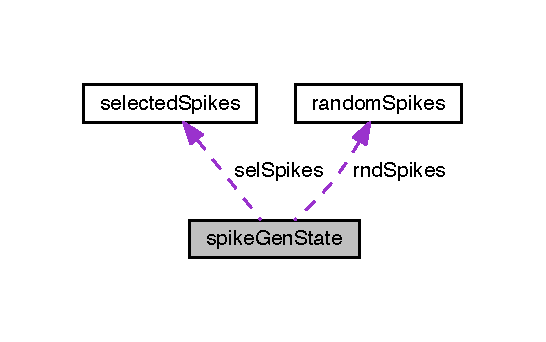
\includegraphics[width=262pt]{structspike_gen_state__coll__graph}
\end{center}
\end{figure}
\subsection*{Data Fields}
\begin{DoxyCompactItemize}
\item 
int \hyperlink{structspike_gen_state_aec7144375204d70824626d74677d71ce}{outboud}
\begin{DoxyCompactList}\small\item\em Represents how many conenctions the input system is attached to in spike\+\_\+generator\+\_\+model\+::outbound. \end{DoxyCompactList}\item 
tw\+\_\+lpid $\ast$ \hyperlink{structspike_gen_state_a569dc67b8984bb0a3616bf17f9763ebb}{connected\+Synapses}
\begin{DoxyCompactList}\small\item\em An array of synapses that this is Random\+Spikes is attached to. \end{DoxyCompactList}\item 
\hyperlink{spike__generator_8h_aa47e87d309aab7727810011578bae86e}{spike\+Gen\+Del} \hyperlink{structspike_gen_state_ae40f21a48f3157bcad074f424046ed2c}{spike\+Gen}
\item 
\hyperlink{structselected_spikes}{selected\+Spikes} \hyperlink{structspike_gen_state_a2da60d116861755bbeeb531a01124cb0}{sel\+Spikes}
\item 
\hyperlink{structrandom_spikes}{random\+Spikes} \hyperlink{structspike_gen_state_a57768e1ceaa4dd88752232ad89b4e8b7}{rnd\+Spikes}
\item 
\hyperlink{spike__generator_8h_ad05574e5624d82eeb7acf436ba8802f6}{random\+Select} \hyperlink{structspike_gen_state_a79f1111d8527d3ef966593c8d389f34d}{gen\+Mode}
\end{DoxyCompactItemize}


\subsection{Detailed Description}
Struct that manages the spike generator. 

Generally, there should be one of these per simulation! 

Definition at line 50 of file spike\+\_\+generator.\+h.



\subsection{Field Documentation}
\hypertarget{structspike_gen_state_a569dc67b8984bb0a3616bf17f9763ebb}{}\index{spike\+Gen\+State@{spike\+Gen\+State}!connected\+Synapses@{connected\+Synapses}}
\index{connected\+Synapses@{connected\+Synapses}!spike\+Gen\+State@{spike\+Gen\+State}}
\subsubsection[{connected\+Synapses}]{\setlength{\rightskip}{0pt plus 5cm}tw\+\_\+lpid$\ast$ connected\+Synapses}\label{structspike_gen_state_a569dc67b8984bb0a3616bf17f9763ebb}


An array of synapses that this is Random\+Spikes is attached to. 



Definition at line 52 of file spike\+\_\+generator.\+h.

\hypertarget{structspike_gen_state_a79f1111d8527d3ef966593c8d389f34d}{}\index{spike\+Gen\+State@{spike\+Gen\+State}!gen\+Mode@{gen\+Mode}}
\index{gen\+Mode@{gen\+Mode}!spike\+Gen\+State@{spike\+Gen\+State}}
\subsubsection[{gen\+Mode}]{\setlength{\rightskip}{0pt plus 5cm}{\bf random\+Select} gen\+Mode}\label{structspike_gen_state_a79f1111d8527d3ef966593c8d389f34d}


Definition at line 57 of file spike\+\_\+generator.\+h.

\hypertarget{structspike_gen_state_aec7144375204d70824626d74677d71ce}{}\index{spike\+Gen\+State@{spike\+Gen\+State}!outboud@{outboud}}
\index{outboud@{outboud}!spike\+Gen\+State@{spike\+Gen\+State}}
\subsubsection[{outboud}]{\setlength{\rightskip}{0pt plus 5cm}int outboud}\label{structspike_gen_state_aec7144375204d70824626d74677d71ce}


Represents how many conenctions the input system is attached to in spike\+\_\+generator\+\_\+model\+::outbound. 



Definition at line 51 of file spike\+\_\+generator.\+h.

\hypertarget{structspike_gen_state_a57768e1ceaa4dd88752232ad89b4e8b7}{}\index{spike\+Gen\+State@{spike\+Gen\+State}!rnd\+Spikes@{rnd\+Spikes}}
\index{rnd\+Spikes@{rnd\+Spikes}!spike\+Gen\+State@{spike\+Gen\+State}}
\subsubsection[{rnd\+Spikes}]{\setlength{\rightskip}{0pt plus 5cm}{\bf random\+Spikes} rnd\+Spikes}\label{structspike_gen_state_a57768e1ceaa4dd88752232ad89b4e8b7}


Definition at line 56 of file spike\+\_\+generator.\+h.

\hypertarget{structspike_gen_state_a2da60d116861755bbeeb531a01124cb0}{}\index{spike\+Gen\+State@{spike\+Gen\+State}!sel\+Spikes@{sel\+Spikes}}
\index{sel\+Spikes@{sel\+Spikes}!spike\+Gen\+State@{spike\+Gen\+State}}
\subsubsection[{sel\+Spikes}]{\setlength{\rightskip}{0pt plus 5cm}{\bf selected\+Spikes} sel\+Spikes}\label{structspike_gen_state_a2da60d116861755bbeeb531a01124cb0}


Definition at line 55 of file spike\+\_\+generator.\+h.

\hypertarget{structspike_gen_state_ae40f21a48f3157bcad074f424046ed2c}{}\index{spike\+Gen\+State@{spike\+Gen\+State}!spike\+Gen@{spike\+Gen}}
\index{spike\+Gen@{spike\+Gen}!spike\+Gen\+State@{spike\+Gen\+State}}
\subsubsection[{spike\+Gen}]{\setlength{\rightskip}{0pt plus 5cm}{\bf spike\+Gen\+Del} spike\+Gen}\label{structspike_gen_state_ae40f21a48f3157bcad074f424046ed2c}


Definition at line 53 of file spike\+\_\+generator.\+h.



The documentation for this struct was generated from the following file\+:\begin{DoxyCompactItemize}
\item 
/\+Users/\+Mark/\+Development/\+True\+North/tnt\+\_\+benchmark/\hyperlink{spike__generator_8h}{spike\+\_\+generator.\+h}\end{DoxyCompactItemize}

\hypertarget{struct_synapse_message}{}\section{Synapse\+Message Struct Reference}
\label{struct_synapse_message}\index{Synapse\+Message@{Synapse\+Message}}


{\ttfamily \#include $<$assist.\+h$>$}



\subsection{Detailed Description}


Definition at line 129 of file assist.\+h.



The documentation for this struct was generated from the following file\+:\begin{DoxyCompactItemize}
\item 
/\+Users/\+Mark/\+Development/\+True\+North/tnt\+\_\+benchmark/\hyperlink{assist_8h}{assist.\+h}\end{DoxyCompactItemize}

\hypertarget{structsynapse_state}{}\section{synapse\+State Struct Reference}
\label{structsynapse_state}\index{synapse\+State@{synapse\+State}}


{\ttfamily \#include $<$synapse.\+h$>$}



Collaboration diagram for synapse\+State\+:\nopagebreak
\begin{figure}[H]
\begin{center}
\leavevmode
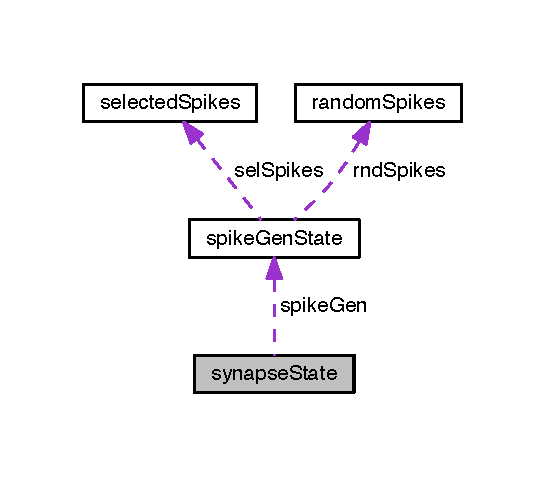
\includegraphics[width=262pt]{structsynapse_state__coll__graph}
\end{center}
\end{figure}
\subsection*{Data Fields}
\begin{DoxyCompactItemize}
\item 
unsigned int \hyperlink{structsynapse_state_aef661be02823d13d471c66bf0cd478db}{syn\+I\+D}
\item 
unsigned int \hyperlink{structsynapse_state_a2063050696509e31bdd72dbb0607c6ee}{core\+I\+D}
\item 
tw\+\_\+lpid $\ast$ \hyperlink{structsynapse_state_a6d6a80692ca06baa6c9a11a624129763}{dests}
\item 
\hyperlink{structspike_gen_state}{spike\+Gen\+State} $\ast$ \hyperlink{structsynapse_state_a11fd4dc41f715eb6f04a68bc5fc9e292}{spike\+Gen}
\end{DoxyCompactItemize}


\subsection{Detailed Description}


Definition at line 17 of file synapse.\+h.



\subsection{Field Documentation}
\hypertarget{structsynapse_state_a2063050696509e31bdd72dbb0607c6ee}{}\index{synapse\+State@{synapse\+State}!core\+I\+D@{core\+I\+D}}
\index{core\+I\+D@{core\+I\+D}!synapse\+State@{synapse\+State}}
\subsubsection[{core\+I\+D}]{\setlength{\rightskip}{0pt plus 5cm}unsigned int core\+I\+D}\label{structsynapse_state_a2063050696509e31bdd72dbb0607c6ee}


Definition at line 19 of file synapse.\+h.

\hypertarget{structsynapse_state_a6d6a80692ca06baa6c9a11a624129763}{}\index{synapse\+State@{synapse\+State}!dests@{dests}}
\index{dests@{dests}!synapse\+State@{synapse\+State}}
\subsubsection[{dests}]{\setlength{\rightskip}{0pt plus 5cm}tw\+\_\+lpid$\ast$ dests}\label{structsynapse_state_a6d6a80692ca06baa6c9a11a624129763}


Definition at line 20 of file synapse.\+h.

\hypertarget{structsynapse_state_a11fd4dc41f715eb6f04a68bc5fc9e292}{}\index{synapse\+State@{synapse\+State}!spike\+Gen@{spike\+Gen}}
\index{spike\+Gen@{spike\+Gen}!synapse\+State@{synapse\+State}}
\subsubsection[{spike\+Gen}]{\setlength{\rightskip}{0pt plus 5cm}{\bf spike\+Gen\+State}$\ast$ spike\+Gen}\label{structsynapse_state_a11fd4dc41f715eb6f04a68bc5fc9e292}


Definition at line 22 of file synapse.\+h.

\hypertarget{structsynapse_state_aef661be02823d13d471c66bf0cd478db}{}\index{synapse\+State@{synapse\+State}!syn\+I\+D@{syn\+I\+D}}
\index{syn\+I\+D@{syn\+I\+D}!synapse\+State@{synapse\+State}}
\subsubsection[{syn\+I\+D}]{\setlength{\rightskip}{0pt plus 5cm}unsigned int syn\+I\+D}\label{structsynapse_state_aef661be02823d13d471c66bf0cd478db}


Definition at line 18 of file synapse.\+h.



The documentation for this struct was generated from the following file\+:\begin{DoxyCompactItemize}
\item 
/\+Users/\+Mark/\+Development/\+True\+North/tnt\+\_\+benchmark/models/\hyperlink{synapse_8h}{synapse.\+h}\end{DoxyCompactItemize}

\chapter{File Documentation}
\hypertarget{assist_8c}{}\section{/home/mplagge/development/tnt\+\_\+benchmark/assist.c File Reference}
\label{assist_8c}\index{/home/mplagge/development/tnt\+\_\+benchmark/assist.\+c@{/home/mplagge/development/tnt\+\_\+benchmark/assist.\+c}}
{\ttfamily \#include \char`\"{}assist.\+h\char`\"{}}\\*
{\ttfamily \#include $<$math.\+h$>$}\\*
Include dependency graph for assist.\+c\+:\nopagebreak
\begin{figure}[H]
\begin{center}
\leavevmode
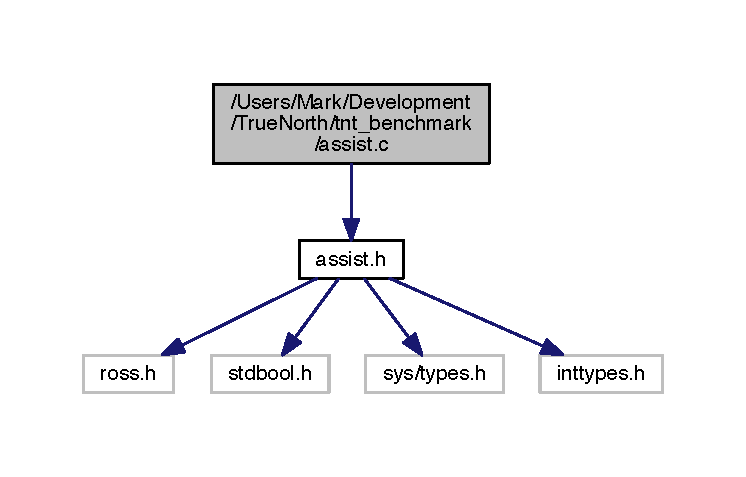
\includegraphics[width=340pt]{assist_8c__incl}
\end{center}
\end{figure}
\subsection*{Functions}
\begin{DoxyCompactItemize}
\item 
tw\+\_\+stime \hyperlink{assist_8c_a30602b11dbfa6bcb90dc00e7942cfb02}{get\+Next\+Event\+Time} (tw\+\_\+lp $\ast$lp)
\begin{DoxyCompactList}\small\item\em Gets the next small-\/tick event time. \end{DoxyCompactList}\item 
tw\+\_\+stime \hyperlink{assist_8c_a4d378196b7fceed090d64ec8820b4065}{get\+Current\+Big\+Tick} (tw\+\_\+stime now)
\begin{DoxyCompactList}\small\item\em Given a tw\+\_\+stime, returns the current big tick. \end{DoxyCompactList}\item 
tw\+\_\+stime \hyperlink{assist_8c_aa961bc9b414f1429b123fc8212c989fd}{get\+Next\+Big\+Tick} (tw\+\_\+stime now)
\begin{DoxyCompactList}\small\item\em Given a tw\+\_\+stime, returns the next big-\/tick that will happen. \end{DoxyCompactList}\end{DoxyCompactItemize}


\subsection{Function Documentation}
\hypertarget{assist_8c_a4d378196b7fceed090d64ec8820b4065}{}\index{assist.\+c@{assist.\+c}!get\+Current\+Big\+Tick@{get\+Current\+Big\+Tick}}
\index{get\+Current\+Big\+Tick@{get\+Current\+Big\+Tick}!assist.\+c@{assist.\+c}}
\subsubsection[{get\+Current\+Big\+Tick}]{\setlength{\rightskip}{0pt plus 5cm}tw\+\_\+stime get\+Current\+Big\+Tick (
\begin{DoxyParamCaption}
\item[{tw\+\_\+stime}]{now}
\end{DoxyParamCaption}
)}\label{assist_8c_a4d378196b7fceed090d64ec8820b4065}


Given a tw\+\_\+stime, returns the current big tick. 

If the time is in-\/between big ticks, this rounds down to the last big tick. There is a bit of a fuzz for times close to the next big tick so if the current time is within \hyperlink{assist_8h_a69434dbcf2196fc2fd1ab7cb57fc9491}{B\+I\+G\+\_\+\+T\+I\+C\+K\+\_\+\+E\+R\+R} of the next big tick, that will be returned instead. Sane parameters would probably be around .000001.\begin{DoxyRefDesc}{Todo}
\item[\hyperlink{todo__todo000001}{Todo}]\+: Implement \& determin if ε needs to be added to the return value.\end{DoxyRefDesc}
\begin{DoxyRefDesc}{Todo}
\item[\hyperlink{todo__todo000002}{Todo}]need to see if this will kill performance\+: \end{DoxyRefDesc}


Definition at line \hyperlink{assist_8c_source_l00030}{30} of file \hyperlink{assist_8c_source}{assist.\+c}.



References \hyperlink{model__main_8h_source_l00063}{C\+O\+R\+E\+\_\+\+S\+I\+Z\+E}.



Referenced by \hyperlink{assist_8c_source_l00041}{get\+Next\+Big\+Tick()}, and \hyperlink{neuron_8c_source_l00028}{linear\+Leak()}.


\begin{DoxyCode}
00030                                         \{
00031     tw\_stime ctick = now / \hyperlink{assist_8h_ad39b86a0b748731175572436f6672264}{CORE\_SIZE};
00033     \textcolor{keywordtype}{long} \textcolor{keywordtype}{double} vtr = 0;
00034     \textcolor{keywordtype}{long} \textcolor{keywordtype}{long} rem = modfl(ctick, &vtr);
00035     \textcolor{comment}{//Rem is current tick, vtr is offset.}
00036 
00037     \textcolor{keywordflow}{return} rem;
00038 
00039 \}
\end{DoxyCode}
\hypertarget{assist_8c_aa961bc9b414f1429b123fc8212c989fd}{}\index{assist.\+c@{assist.\+c}!get\+Next\+Big\+Tick@{get\+Next\+Big\+Tick}}
\index{get\+Next\+Big\+Tick@{get\+Next\+Big\+Tick}!assist.\+c@{assist.\+c}}
\subsubsection[{get\+Next\+Big\+Tick}]{\setlength{\rightskip}{0pt plus 5cm}tw\+\_\+stime get\+Next\+Big\+Tick (
\begin{DoxyParamCaption}
\item[{tw\+\_\+stime}]{now}
\end{DoxyParamCaption}
)}\label{assist_8c_aa961bc9b414f1429b123fc8212c989fd}


Given a tw\+\_\+stime, returns the next big-\/tick that will happen. 


\begin{DoxyParams}{Parameters}
{\em now} & Right now!\\
\hline
\end{DoxyParams}
\begin{DoxyReturn}{Returns}
Next big tick time. 
\end{DoxyReturn}


Definition at line \hyperlink{assist_8c_source_l00041}{41} of file \hyperlink{assist_8c_source}{assist.\+c}.



References \hyperlink{model__main_8h_source_l00063}{C\+O\+R\+E\+\_\+\+S\+I\+Z\+E}, and \hyperlink{assist_8c_source_l00030}{get\+Current\+Big\+Tick()}.



Referenced by \hyperlink{neuron_8c_source_l00167}{neuron\+Fire()}, and \hyperlink{neuron_8c_source_l00179}{send\+Heartbeat()}.


\begin{DoxyCode}
00041                                       \{
00042     \textcolor{keywordtype}{long} \textcolor{keywordtype}{long} curr = \hyperlink{assist_8h_ad39b86a0b748731175572436f6672264}{CORE\_SIZE} * \hyperlink{assist_8c_a4d378196b7fceed090d64ec8820b4065}{getCurrentBigTick}(now) + 1;
00043     \textcolor{keywordflow}{return} curr - now;
00044 
00045         \textcolor{comment}{//Need to figure this out - not accurate until this is done:}
00046 
00047 \}\end{DoxyCode}


Here is the call graph for this function\+:\nopagebreak
\begin{figure}[H]
\begin{center}
\leavevmode
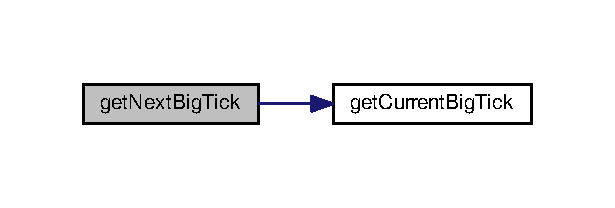
\includegraphics[width=295pt]{assist_8c_aa961bc9b414f1429b123fc8212c989fd_cgraph}
\end{center}
\end{figure}


\hypertarget{assist_8c_a30602b11dbfa6bcb90dc00e7942cfb02}{}\index{assist.\+c@{assist.\+c}!get\+Next\+Event\+Time@{get\+Next\+Event\+Time}}
\index{get\+Next\+Event\+Time@{get\+Next\+Event\+Time}!assist.\+c@{assist.\+c}}
\subsubsection[{get\+Next\+Event\+Time}]{\setlength{\rightskip}{0pt plus 5cm}tw\+\_\+stime get\+Next\+Event\+Time (
\begin{DoxyParamCaption}
\item[{tw\+\_\+lp $\ast$}]{lp}
\end{DoxyParamCaption}
)}\label{assist_8c_a30602b11dbfa6bcb90dc00e7942cfb02}


Gets the next small-\/tick event time. 

Gets the next event time, based on a random function. 

Definition at line \hyperlink{assist_8c_source_l00014}{14} of file \hyperlink{assist_8c_source}{assist.\+c}.



Referenced by \hyperlink{axon_8c_source_l00011}{axon\+Receive\+Message()}, and \hyperlink{synapse_8c_source_l00011}{synapse\+Receive\+Message()}.


\begin{DoxyCode}
00014                                     \{
00015 
00016     tw\_stime r =tw\_rand\_unif(lp->rng) / 10;
00017 
00018     \textcolor{keywordflow}{return} r;
00019 
00020 \}
\end{DoxyCode}

\hypertarget{assist_8h}{}\section{/\+Users/\+Mark/\+Development/\+True\+North/tnt\+\_\+benchmark/assist.h File Reference}
\label{assist_8h}\index{/\+Users/\+Mark/\+Development/\+True\+North/tnt\+\_\+benchmark/assist.\+h@{/\+Users/\+Mark/\+Development/\+True\+North/tnt\+\_\+benchmark/assist.\+h}}
{\ttfamily \#include $<$stdio.\+h$>$}\\*
{\ttfamily \#include $<$inttypes.\+h$>$}\\*
{\ttfamily \#include $<$stdbool.\+h$>$}\\*
{\ttfamily \#include \char`\"{}ross.\+h\char`\"{}}\\*
Include dependency graph for assist.\+h\+:
\nopagebreak
\begin{figure}[H]
\begin{center}
\leavevmode
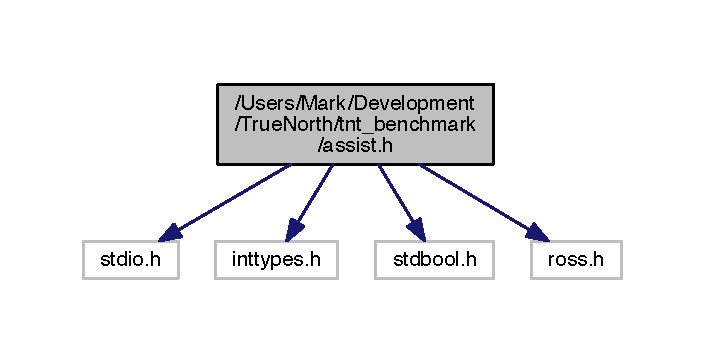
\includegraphics[width=338pt]{assist_8h__incl}
\end{center}
\end{figure}
This graph shows which files directly or indirectly include this file\+:
\nopagebreak
\begin{figure}[H]
\begin{center}
\leavevmode
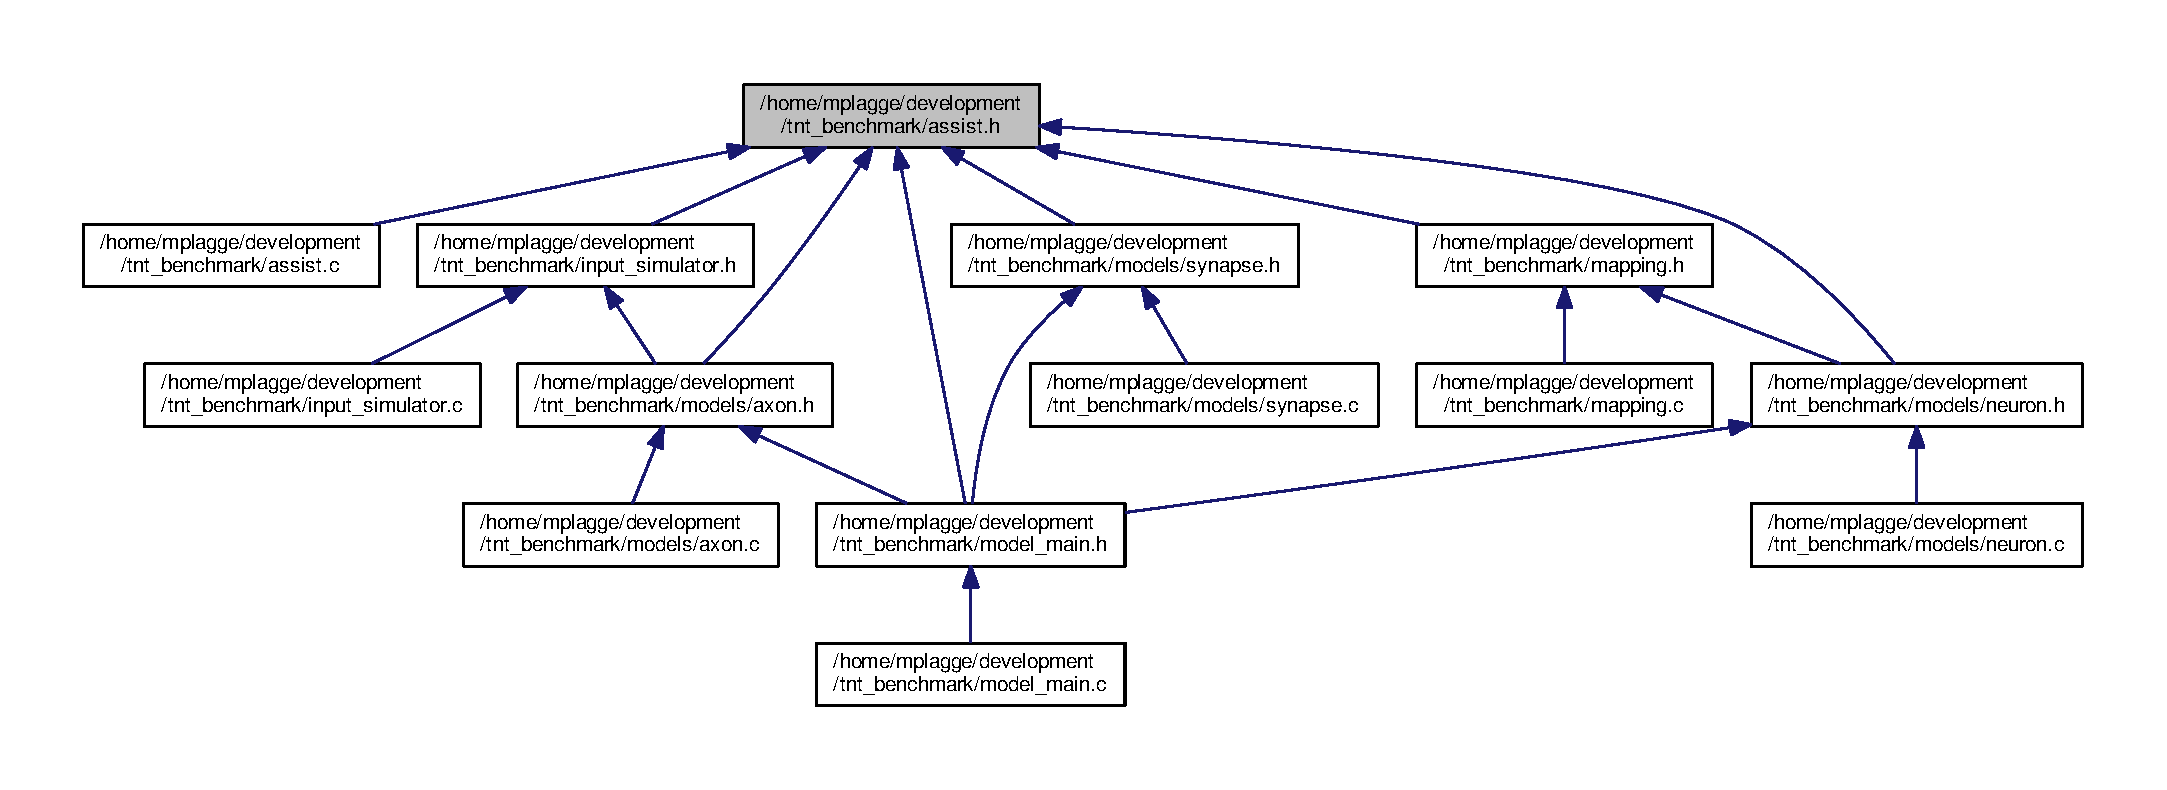
\includegraphics[width=350pt]{assist_8h__dep__incl}
\end{center}
\end{figure}
\subsection*{Data Structures}
\begin{DoxyCompactItemize}
\item 
struct \hyperlink{struct_msg___data}{Msg\+\_\+\+Data}
\begin{DoxyCompactList}\small\item\em Main message struct. \end{DoxyCompactList}\end{DoxyCompactItemize}
\subsection*{Macros}
\begin{DoxyCompactItemize}
\item 
\#define \hyperlink{assist_8h_a3f7a6e6a1210b6d9d7a42177dcb9634b}{\+\_\+id\+T}~uint\+\_\+fast32\+\_\+t
\item 
\#define \hyperlink{assist_8h_abe1fc1b8f9efd1187e564bcb8de7f815}{\+\_\+volt\+T}~int\+\_\+fast32\+\_\+t
\item 
\#define \hyperlink{assist_8h_ad77e6fc5a9b03d46e7c97b7c4b92e89f}{\+\_\+stat\+T}~int\+\_\+fast64\+\_\+t
\item 
\#define \hyperlink{assist_8h_abd3130ec511af0cc7768768554bd36a0}{\+\_\+reg\+I\+D\+T}~uint32\+\_\+t
\begin{DoxyCompactList}\small\item\em \+\_\+reg\+I\+D\+T is a \char`\"{}regional id\char`\"{} type. \end{DoxyCompactList}\item 
\#define \hyperlink{assist_8h_aaf4b596256d346dd40bc6f14c3eb9371}{I\+A\+B\+S}(a)~(((a) $<$ 0) ? (-\/a) \+: (a))
\begin{DoxyCompactList}\small\item\em I\+A\+B\+S is an integer absolute value function. \end{DoxyCompactList}\item 
\#define \hyperlink{assist_8h_ad383c153e77508e2556003da0e4ac3eb}{R\+Z\+E\+R}(a)~(((a) $<$ 0) ? (0) \+: (a))
\begin{DoxyCompactList}\small\item\em R\+Z\+E\+R is a floor function -\/ values below zero round up to zero. \end{DoxyCompactList}\end{DoxyCompactItemize}
\subsection*{Enumerations}
\begin{DoxyCompactItemize}
\item 
enum \hyperlink{assist_8h_a7c1688de451e0dea1e11617bce3ec450}{evt\+Type} \{ \\*
\hyperlink{assist_8h_a7c1688de451e0dea1e11617bce3ec450abb8b28588ca2e1c33d29df003b3b90ee}{A\+X\+O\+N\+\_\+\+O\+U\+T}, 
\hyperlink{assist_8h_a7c1688de451e0dea1e11617bce3ec450a9afa7ee7839cdd980f348a3a70b0054f}{A\+X\+O\+N\+\_\+\+H\+E\+A\+R\+T\+B\+E\+A\+T}, 
\hyperlink{assist_8h_a7c1688de451e0dea1e11617bce3ec450a6ad6b93d8a818550e7246f6e0d143afb}{S\+Y\+N\+A\+P\+S\+E\+\_\+\+O\+U\+T}, 
\hyperlink{assist_8h_a7c1688de451e0dea1e11617bce3ec450a777cedd6ca25a5d7a84aab10a8735af0}{N\+E\+U\+R\+O\+N\+\_\+\+O\+U\+T}, 
\\*
\hyperlink{assist_8h_a7c1688de451e0dea1e11617bce3ec450a226690009a653238a52339561e6c466e}{N\+E\+U\+R\+O\+N\+\_\+\+H\+E\+A\+R\+T\+B\+E\+A\+T}, 
\hyperlink{assist_8h_a7c1688de451e0dea1e11617bce3ec450add78176054e14835c454b5f2d1827d42}{G\+E\+N\+\_\+\+H\+E\+A\+R\+T\+B\+E\+A\+T}
 \}
\begin{DoxyCompactList}\small\item\em evt\+Type is a message/event identifier flag \end{DoxyCompactList}\end{DoxyCompactItemize}
\subsection*{Functions}
\begin{DoxyCompactItemize}
\item 
tw\+\_\+stime \hyperlink{assist_8h_a30602b11dbfa6bcb90dc00e7942cfb02}{get\+Next\+Event\+Time} (tw\+\_\+lp $\ast$lp)
\begin{DoxyCompactList}\small\item\em Gets the next event time, based on a random function. \end{DoxyCompactList}\end{DoxyCompactItemize}
\subsection*{Variables}
\begin{DoxyCompactItemize}
\item 
int \hyperlink{assist_8h_a67e8e45768f76b984a60fcff2b7c51aa}{N\+E\+U\+R\+O\+N\+S\+\_\+\+I\+N\+\_\+\+C\+O\+R\+E}
\begin{DoxyCompactList}\small\item\em Number of neurons per core. \end{DoxyCompactList}\item 
int \hyperlink{assist_8h_a142b2655c5a899956164ef4e1c394fea}{C\+O\+R\+E\+S\+\_\+\+I\+N\+\_\+\+S\+I\+M}
\item 
int \hyperlink{assist_8h_a519a06367b2b3f793c56d3ab78f5b2ef}{A\+X\+O\+N\+S\+\_\+\+I\+N\+\_\+\+C\+O\+R\+E}
\begin{DoxyCompactList}\small\item\em Number of axions per core. \end{DoxyCompactList}\item 
int \hyperlink{assist_8h_a076b99099b46431255982b2bb8ce06fb}{S\+Y\+N\+A\+P\+S\+E\+S\+\_\+\+I\+N\+\_\+\+C\+O\+R\+E}
\item 
unsigned int \hyperlink{assist_8h_a74019486208bb1d640927710d5344a94}{G\+E\+N\+\_\+\+O\+N}
\begin{DoxyCompactList}\small\item\em Simulation tuning variables. \end{DoxyCompactList}\item 
bool \hyperlink{assist_8h_ab42fd7d6d043114d1147acc77bd7e867}{G\+E\+N\+\_\+\+R\+N\+D}
\item 
unsigned int \hyperlink{assist_8h_a516f1496efbe86dedb0e2883bb7e7834}{R\+N\+D\+\_\+\+M\+O\+D\+E}
\item 
unsigned int \hyperlink{assist_8h_a4875b976acd12ff43cc03898be994253}{G\+E\+N\+\_\+\+P\+R\+O\+B}
\item 
unsigned int \hyperlink{assist_8h_a3ba8de640782035ea9e91ab791d9f14f}{G\+E\+N\+\_\+\+F\+C\+T}
\item 
unsigned int \hyperlink{assist_8h_a6f8efb1b6d497ba57f27acadae57dc4b}{G\+E\+N\+\_\+\+O\+U\+T\+B\+O\+U\+N\+D}
\item 
unsigned int \hyperlink{assist_8h_ab161ae8a99d41559eba4ab3dd8d69218}{G\+E\+N\+\_\+\+S\+E\+L\+\_\+\+M\+O\+D\+E}
\item 
unsigned int \hyperlink{assist_8h_a0a9f8592bd29be6c5c7433c3c0bf42dd}{S\+P\+\_\+\+D\+B\+G}
\item 
int \hyperlink{assist_8h_a433873baf41da436ba9c1734c8c5ddd2}{T\+H\+R\+E\+S\+H\+O\+L\+D\+\_\+\+M\+A\+X}
\begin{DoxyCompactList}\small\item\em Determines the maximum and minimum thresholds for a neuron to fire. \end{DoxyCompactList}\item 
int \hyperlink{assist_8h_a55f4484944f4174b5e677c0a71b30e4a}{T\+H\+R\+E\+S\+H\+O\+L\+D\+\_\+\+M\+I\+N}
\begin{DoxyCompactList}\small\item\em Minimum threshold. \end{DoxyCompactList}\item 
int \hyperlink{assist_8h_a20ef6d41d2f384358522fb59fb6226cb}{S\+Y\+N\+A\+P\+S\+E\+\_\+\+W\+E\+I\+G\+H\+T\+\_\+\+M\+A\+X}
\begin{DoxyCompactList}\small\item\em Each neuron is connected to the synapses (inputs) within the core it is running in. \end{DoxyCompactList}\item 
int \hyperlink{assist_8h_af38a0e2e2483ef81f7ea5175c366ce82}{S\+Y\+N\+A\+P\+S\+E\+\_\+\+W\+E\+I\+G\+H\+T\+\_\+\+M\+I\+N}
\begin{DoxyCompactList}\small\item\em Minimum synapse weight. \end{DoxyCompactList}\item 
int \hyperlink{assist_8h_ad39b86a0b748731175572436f6672264}{C\+O\+R\+E\+\_\+\+S\+I\+Z\+E}
\begin{DoxyCompactList}\small\item\em C\+O\+R\+E\+\_\+\+S\+I\+Z\+E is equal to the number of axions $\ast$ number of aneurons + num neurons + num axions. \end{DoxyCompactList}\end{DoxyCompactItemize}


\subsection{Macro Definition Documentation}
\hypertarget{assist_8h_a3f7a6e6a1210b6d9d7a42177dcb9634b}{}\index{assist.\+h@{assist.\+h}!\+\_\+id\+T@{\+\_\+id\+T}}
\index{\+\_\+id\+T@{\+\_\+id\+T}!assist.\+h@{assist.\+h}}
\subsubsection[{\+\_\+id\+T}]{\setlength{\rightskip}{0pt plus 5cm}\#define \+\_\+id\+T~uint\+\_\+fast32\+\_\+t}\label{assist_8h_a3f7a6e6a1210b6d9d7a42177dcb9634b}


Definition at line \hyperlink{assist_8h_source_l00018}{18} of file \hyperlink{assist_8h_source}{assist.\+h}.

\hypertarget{assist_8h_abd3130ec511af0cc7768768554bd36a0}{}\index{assist.\+h@{assist.\+h}!\+\_\+reg\+I\+D\+T@{\+\_\+reg\+I\+D\+T}}
\index{\+\_\+reg\+I\+D\+T@{\+\_\+reg\+I\+D\+T}!assist.\+h@{assist.\+h}}
\subsubsection[{\+\_\+reg\+I\+D\+T}]{\setlength{\rightskip}{0pt plus 5cm}\#define \+\_\+reg\+I\+D\+T~uint32\+\_\+t}\label{assist_8h_abd3130ec511af0cc7768768554bd36a0}


\+\_\+reg\+I\+D\+T is a \char`\"{}regional id\char`\"{} type. 

This variable type is for storing core\+I\+Ds and local\+I\+Ds. It must be half the bit size of tw\+\_\+lpid.\begin{DoxyRefDesc}{Todo}
\item[\hyperlink{todo__todo000001}{Todo}]\+: add macro to adjust the bit width. \end{DoxyRefDesc}


Definition at line \hyperlink{assist_8h_source_l00024}{24} of file \hyperlink{assist_8h_source}{assist.\+h}.

\hypertarget{assist_8h_ad77e6fc5a9b03d46e7c97b7c4b92e89f}{}\index{assist.\+h@{assist.\+h}!\+\_\+stat\+T@{\+\_\+stat\+T}}
\index{\+\_\+stat\+T@{\+\_\+stat\+T}!assist.\+h@{assist.\+h}}
\subsubsection[{\+\_\+stat\+T}]{\setlength{\rightskip}{0pt plus 5cm}\#define \+\_\+stat\+T~int\+\_\+fast64\+\_\+t}\label{assist_8h_ad77e6fc5a9b03d46e7c97b7c4b92e89f}


Definition at line \hyperlink{assist_8h_source_l00020}{20} of file \hyperlink{assist_8h_source}{assist.\+h}.

\hypertarget{assist_8h_abe1fc1b8f9efd1187e564bcb8de7f815}{}\index{assist.\+h@{assist.\+h}!\+\_\+volt\+T@{\+\_\+volt\+T}}
\index{\+\_\+volt\+T@{\+\_\+volt\+T}!assist.\+h@{assist.\+h}}
\subsubsection[{\+\_\+volt\+T}]{\setlength{\rightskip}{0pt plus 5cm}\#define \+\_\+volt\+T~int\+\_\+fast32\+\_\+t}\label{assist_8h_abe1fc1b8f9efd1187e564bcb8de7f815}


Definition at line \hyperlink{assist_8h_source_l00019}{19} of file \hyperlink{assist_8h_source}{assist.\+h}.

\hypertarget{assist_8h_aaf4b596256d346dd40bc6f14c3eb9371}{}\index{assist.\+h@{assist.\+h}!I\+A\+B\+S@{I\+A\+B\+S}}
\index{I\+A\+B\+S@{I\+A\+B\+S}!assist.\+h@{assist.\+h}}
\subsubsection[{I\+A\+B\+S}]{\setlength{\rightskip}{0pt plus 5cm}\#define I\+A\+B\+S(
\begin{DoxyParamCaption}
\item[{}]{a}
\end{DoxyParamCaption}
)~(((a) $<$ 0) ? (-\/a) \+: (a))}\label{assist_8h_aaf4b596256d346dd40bc6f14c3eb9371}


I\+A\+B\+S is an integer absolute value function. 



Definition at line \hyperlink{assist_8h_source_l00029}{29} of file \hyperlink{assist_8h_source}{assist.\+h}.

\hypertarget{assist_8h_ad383c153e77508e2556003da0e4ac3eb}{}\index{assist.\+h@{assist.\+h}!R\+Z\+E\+R@{R\+Z\+E\+R}}
\index{R\+Z\+E\+R@{R\+Z\+E\+R}!assist.\+h@{assist.\+h}}
\subsubsection[{R\+Z\+E\+R}]{\setlength{\rightskip}{0pt plus 5cm}\#define R\+Z\+E\+R(
\begin{DoxyParamCaption}
\item[{}]{a}
\end{DoxyParamCaption}
)~(((a) $<$ 0) ? (0) \+: (a))}\label{assist_8h_ad383c153e77508e2556003da0e4ac3eb}


R\+Z\+E\+R is a floor function -\/ values below zero round up to zero. 



Definition at line \hyperlink{assist_8h_source_l00031}{31} of file \hyperlink{assist_8h_source}{assist.\+h}.



\subsection{Enumeration Type Documentation}
\hypertarget{assist_8h_a7c1688de451e0dea1e11617bce3ec450}{}\index{assist.\+h@{assist.\+h}!evt\+Type@{evt\+Type}}
\index{evt\+Type@{evt\+Type}!assist.\+h@{assist.\+h}}
\subsubsection[{evt\+Type}]{\setlength{\rightskip}{0pt plus 5cm}enum {\bf evt\+Type}}\label{assist_8h_a7c1688de451e0dea1e11617bce3ec450}


evt\+Type is a message/event identifier flag 

\begin{Desc}
\item[Enumerator]\par
\begin{description}
\index{A\+X\+O\+N\+\_\+\+O\+U\+T@{A\+X\+O\+N\+\_\+\+O\+U\+T}!assist.\+h@{assist.\+h}}\index{assist.\+h@{assist.\+h}!A\+X\+O\+N\+\_\+\+O\+U\+T@{A\+X\+O\+N\+\_\+\+O\+U\+T}}\item[{\em 
\hypertarget{assist_8h_a7c1688de451e0dea1e11617bce3ec450abb8b28588ca2e1c33d29df003b3b90ee}{}A\+X\+O\+N\+\_\+\+O\+U\+T\label{assist_8h_a7c1688de451e0dea1e11617bce3ec450abb8b28588ca2e1c33d29df003b3b90ee}
}]\index{A\+X\+O\+N\+\_\+\+H\+E\+A\+R\+T\+B\+E\+A\+T@{A\+X\+O\+N\+\_\+\+H\+E\+A\+R\+T\+B\+E\+A\+T}!assist.\+h@{assist.\+h}}\index{assist.\+h@{assist.\+h}!A\+X\+O\+N\+\_\+\+H\+E\+A\+R\+T\+B\+E\+A\+T@{A\+X\+O\+N\+\_\+\+H\+E\+A\+R\+T\+B\+E\+A\+T}}\item[{\em 
\hypertarget{assist_8h_a7c1688de451e0dea1e11617bce3ec450a9afa7ee7839cdd980f348a3a70b0054f}{}A\+X\+O\+N\+\_\+\+H\+E\+A\+R\+T\+B\+E\+A\+T\label{assist_8h_a7c1688de451e0dea1e11617bce3ec450a9afa7ee7839cdd980f348a3a70b0054f}
}]Message originates from an axon. \index{S\+Y\+N\+A\+P\+S\+E\+\_\+\+O\+U\+T@{S\+Y\+N\+A\+P\+S\+E\+\_\+\+O\+U\+T}!assist.\+h@{assist.\+h}}\index{assist.\+h@{assist.\+h}!S\+Y\+N\+A\+P\+S\+E\+\_\+\+O\+U\+T@{S\+Y\+N\+A\+P\+S\+E\+\_\+\+O\+U\+T}}\item[{\em 
\hypertarget{assist_8h_a7c1688de451e0dea1e11617bce3ec450a6ad6b93d8a818550e7246f6e0d143afb}{}S\+Y\+N\+A\+P\+S\+E\+\_\+\+O\+U\+T\label{assist_8h_a7c1688de451e0dea1e11617bce3ec450a6ad6b93d8a818550e7246f6e0d143afb}
}]Axon heartbeat message -\/ big clock synchronization. \index{N\+E\+U\+R\+O\+N\+\_\+\+O\+U\+T@{N\+E\+U\+R\+O\+N\+\_\+\+O\+U\+T}!assist.\+h@{assist.\+h}}\index{assist.\+h@{assist.\+h}!N\+E\+U\+R\+O\+N\+\_\+\+O\+U\+T@{N\+E\+U\+R\+O\+N\+\_\+\+O\+U\+T}}\item[{\em 
\hypertarget{assist_8h_a7c1688de451e0dea1e11617bce3ec450a777cedd6ca25a5d7a84aab10a8735af0}{}N\+E\+U\+R\+O\+N\+\_\+\+O\+U\+T\label{assist_8h_a7c1688de451e0dea1e11617bce3ec450a777cedd6ca25a5d7a84aab10a8735af0}
}]Message originates from a synapse. \index{N\+E\+U\+R\+O\+N\+\_\+\+H\+E\+A\+R\+T\+B\+E\+A\+T@{N\+E\+U\+R\+O\+N\+\_\+\+H\+E\+A\+R\+T\+B\+E\+A\+T}!assist.\+h@{assist.\+h}}\index{assist.\+h@{assist.\+h}!N\+E\+U\+R\+O\+N\+\_\+\+H\+E\+A\+R\+T\+B\+E\+A\+T@{N\+E\+U\+R\+O\+N\+\_\+\+H\+E\+A\+R\+T\+B\+E\+A\+T}}\item[{\em 
\hypertarget{assist_8h_a7c1688de451e0dea1e11617bce3ec450a226690009a653238a52339561e6c466e}{}N\+E\+U\+R\+O\+N\+\_\+\+H\+E\+A\+R\+T\+B\+E\+A\+T\label{assist_8h_a7c1688de451e0dea1e11617bce3ec450a226690009a653238a52339561e6c466e}
}]Message originates from a neuron, and is going to an axion. \index{G\+E\+N\+\_\+\+H\+E\+A\+R\+T\+B\+E\+A\+T@{G\+E\+N\+\_\+\+H\+E\+A\+R\+T\+B\+E\+A\+T}!assist.\+h@{assist.\+h}}\index{assist.\+h@{assist.\+h}!G\+E\+N\+\_\+\+H\+E\+A\+R\+T\+B\+E\+A\+T@{G\+E\+N\+\_\+\+H\+E\+A\+R\+T\+B\+E\+A\+T}}\item[{\em 
\hypertarget{assist_8h_a7c1688de451e0dea1e11617bce3ec450add78176054e14835c454b5f2d1827d42}{}G\+E\+N\+\_\+\+H\+E\+A\+R\+T\+B\+E\+A\+T\label{assist_8h_a7c1688de451e0dea1e11617bce3ec450add78176054e14835c454b5f2d1827d42}
}]Neuron heartbeat messages -\/ for big clock syncronization. Signal generator messages -- used to simulate input for benchmarking. \end{description}
\end{Desc}


Definition at line \hyperlink{assist_8h_source_l00035}{35} of file \hyperlink{assist_8h_source}{assist.\+h}.


\begin{DoxyCode}
00035              \{
00036     \hyperlink{assist_8h_a7c1688de451e0dea1e11617bce3ec450abb8b28588ca2e1c33d29df003b3b90ee}{AXON\_OUT}, 
00037     \hyperlink{assist_8h_a7c1688de451e0dea1e11617bce3ec450a9afa7ee7839cdd980f348a3a70b0054f}{AXON\_HEARTBEAT}, 
00038     \hyperlink{assist_8h_a7c1688de451e0dea1e11617bce3ec450a6ad6b93d8a818550e7246f6e0d143afb}{SYNAPSE\_OUT}, 
00039     \hyperlink{assist_8h_a7c1688de451e0dea1e11617bce3ec450a777cedd6ca25a5d7a84aab10a8735af0}{NEURON\_OUT}, 
00040     \hyperlink{assist_8h_a7c1688de451e0dea1e11617bce3ec450a226690009a653238a52339561e6c466e}{NEURON\_HEARTBEAT}, 
00041     \hyperlink{assist_8h_a7c1688de451e0dea1e11617bce3ec450add78176054e14835c454b5f2d1827d42}{GEN\_HEARTBEAT} 
00042 \};
\end{DoxyCode}


\subsection{Function Documentation}
\hypertarget{assist_8h_a30602b11dbfa6bcb90dc00e7942cfb02}{}\index{assist.\+h@{assist.\+h}!get\+Next\+Event\+Time@{get\+Next\+Event\+Time}}
\index{get\+Next\+Event\+Time@{get\+Next\+Event\+Time}!assist.\+h@{assist.\+h}}
\subsubsection[{get\+Next\+Event\+Time}]{\setlength{\rightskip}{0pt plus 5cm}tw\+\_\+stime get\+Next\+Event\+Time (
\begin{DoxyParamCaption}
\item[{tw\+\_\+lp $\ast$}]{lp}
\end{DoxyParamCaption}
)}\label{assist_8h_a30602b11dbfa6bcb90dc00e7942cfb02}


Gets the next event time, based on a random function. 

Moved here to allow for easier abstraciton, and random function replacement.


\begin{DoxyParams}{Parameters}
{\em lp} & Reference to the current L\+P so that the function can see the R\+N\+G\\
\hline
\end{DoxyParams}
\begin{DoxyReturn}{Returns}
a tw\+\_\+stime value, such that $ 0 < t < 1 $. A delta for the next time slice. 
\end{DoxyReturn}


Definition at line \hyperlink{assist_8c_source_l00020}{20} of file \hyperlink{assist_8c_source}{assist.\+c}.


\begin{DoxyCode}
00020                                     \{
00021 
00022     tw\_stime r =tw\_rand\_unif(lp->rng) / 10;
00023 
00024     \textcolor{keywordflow}{return} r;
00025 
00026 \}\end{DoxyCode}


\subsection{Variable Documentation}
\hypertarget{assist_8h_a519a06367b2b3f793c56d3ab78f5b2ef}{}\index{assist.\+h@{assist.\+h}!A\+X\+O\+N\+S\+\_\+\+I\+N\+\_\+\+C\+O\+R\+E@{A\+X\+O\+N\+S\+\_\+\+I\+N\+\_\+\+C\+O\+R\+E}}
\index{A\+X\+O\+N\+S\+\_\+\+I\+N\+\_\+\+C\+O\+R\+E@{A\+X\+O\+N\+S\+\_\+\+I\+N\+\_\+\+C\+O\+R\+E}!assist.\+h@{assist.\+h}}
\subsubsection[{A\+X\+O\+N\+S\+\_\+\+I\+N\+\_\+\+C\+O\+R\+E}]{\setlength{\rightskip}{0pt plus 5cm}int A\+X\+O\+N\+S\+\_\+\+I\+N\+\_\+\+C\+O\+R\+E}\label{assist_8h_a519a06367b2b3f793c56d3ab78f5b2ef}


Number of axions per core. 

Generally is set to 1-\/1 with neurons in core 

Definition at line \hyperlink{model__main_8h_source_l00029}{29} of file \hyperlink{model__main_8h_source}{model\+\_\+main.\+h}.

\hypertarget{assist_8h_ad39b86a0b748731175572436f6672264}{}\index{assist.\+h@{assist.\+h}!C\+O\+R\+E\+\_\+\+S\+I\+Z\+E@{C\+O\+R\+E\+\_\+\+S\+I\+Z\+E}}
\index{C\+O\+R\+E\+\_\+\+S\+I\+Z\+E@{C\+O\+R\+E\+\_\+\+S\+I\+Z\+E}!assist.\+h@{assist.\+h}}
\subsubsection[{C\+O\+R\+E\+\_\+\+S\+I\+Z\+E}]{\setlength{\rightskip}{0pt plus 5cm}int C\+O\+R\+E\+\_\+\+S\+I\+Z\+E}\label{assist_8h_ad39b86a0b748731175572436f6672264}


C\+O\+R\+E\+\_\+\+S\+I\+Z\+E is equal to the number of axions $\ast$ number of aneurons + num neurons + num axions. 



Definition at line \hyperlink{model__main_8h_source_l00063}{63} of file \hyperlink{model__main_8h_source}{model\+\_\+main.\+h}.

\hypertarget{assist_8h_a142b2655c5a899956164ef4e1c394fea}{}\index{assist.\+h@{assist.\+h}!C\+O\+R\+E\+S\+\_\+\+I\+N\+\_\+\+S\+I\+M@{C\+O\+R\+E\+S\+\_\+\+I\+N\+\_\+\+S\+I\+M}}
\index{C\+O\+R\+E\+S\+\_\+\+I\+N\+\_\+\+S\+I\+M@{C\+O\+R\+E\+S\+\_\+\+I\+N\+\_\+\+S\+I\+M}!assist.\+h@{assist.\+h}}
\subsubsection[{C\+O\+R\+E\+S\+\_\+\+I\+N\+\_\+\+S\+I\+M}]{\setlength{\rightskip}{0pt plus 5cm}int C\+O\+R\+E\+S\+\_\+\+I\+N\+\_\+\+S\+I\+M}\label{assist_8h_a142b2655c5a899956164ef4e1c394fea}


Definition at line \hyperlink{model__main_8h_source_l00026}{26} of file \hyperlink{model__main_8h_source}{model\+\_\+main.\+h}.

\hypertarget{assist_8h_a3ba8de640782035ea9e91ab791d9f14f}{}\index{assist.\+h@{assist.\+h}!G\+E\+N\+\_\+\+F\+C\+T@{G\+E\+N\+\_\+\+F\+C\+T}}
\index{G\+E\+N\+\_\+\+F\+C\+T@{G\+E\+N\+\_\+\+F\+C\+T}!assist.\+h@{assist.\+h}}
\subsubsection[{G\+E\+N\+\_\+\+F\+C\+T}]{\setlength{\rightskip}{0pt plus 5cm}unsigned int G\+E\+N\+\_\+\+F\+C\+T}\label{assist_8h_a3ba8de640782035ea9e91ab791d9f14f}


Definition at line \hyperlink{model__main_8h_source_l00038}{38} of file \hyperlink{model__main_8h_source}{model\+\_\+main.\+h}.

\hypertarget{assist_8h_a74019486208bb1d640927710d5344a94}{}\index{assist.\+h@{assist.\+h}!G\+E\+N\+\_\+\+O\+N@{G\+E\+N\+\_\+\+O\+N}}
\index{G\+E\+N\+\_\+\+O\+N@{G\+E\+N\+\_\+\+O\+N}!assist.\+h@{assist.\+h}}
\subsubsection[{G\+E\+N\+\_\+\+O\+N}]{\setlength{\rightskip}{0pt plus 5cm}unsigned int G\+E\+N\+\_\+\+O\+N}\label{assist_8h_a74019486208bb1d640927710d5344a94}


Simulation tuning variables. 

noise generator values 

Definition at line \hyperlink{model__main_8h_source_l00034}{34} of file \hyperlink{model__main_8h_source}{model\+\_\+main.\+h}.

\hypertarget{assist_8h_a6f8efb1b6d497ba57f27acadae57dc4b}{}\index{assist.\+h@{assist.\+h}!G\+E\+N\+\_\+\+O\+U\+T\+B\+O\+U\+N\+D@{G\+E\+N\+\_\+\+O\+U\+T\+B\+O\+U\+N\+D}}
\index{G\+E\+N\+\_\+\+O\+U\+T\+B\+O\+U\+N\+D@{G\+E\+N\+\_\+\+O\+U\+T\+B\+O\+U\+N\+D}!assist.\+h@{assist.\+h}}
\subsubsection[{G\+E\+N\+\_\+\+O\+U\+T\+B\+O\+U\+N\+D}]{\setlength{\rightskip}{0pt plus 5cm}unsigned int G\+E\+N\+\_\+\+O\+U\+T\+B\+O\+U\+N\+D}\label{assist_8h_a6f8efb1b6d497ba57f27acadae57dc4b}


Definition at line \hyperlink{model__main_8h_source_l00039}{39} of file \hyperlink{model__main_8h_source}{model\+\_\+main.\+h}.

\hypertarget{assist_8h_a4875b976acd12ff43cc03898be994253}{}\index{assist.\+h@{assist.\+h}!G\+E\+N\+\_\+\+P\+R\+O\+B@{G\+E\+N\+\_\+\+P\+R\+O\+B}}
\index{G\+E\+N\+\_\+\+P\+R\+O\+B@{G\+E\+N\+\_\+\+P\+R\+O\+B}!assist.\+h@{assist.\+h}}
\subsubsection[{G\+E\+N\+\_\+\+P\+R\+O\+B}]{\setlength{\rightskip}{0pt plus 5cm}unsigned int G\+E\+N\+\_\+\+P\+R\+O\+B}\label{assist_8h_a4875b976acd12ff43cc03898be994253}


Definition at line \hyperlink{model__main_8h_source_l00037}{37} of file \hyperlink{model__main_8h_source}{model\+\_\+main.\+h}.

\hypertarget{assist_8h_ab42fd7d6d043114d1147acc77bd7e867}{}\index{assist.\+h@{assist.\+h}!G\+E\+N\+\_\+\+R\+N\+D@{G\+E\+N\+\_\+\+R\+N\+D}}
\index{G\+E\+N\+\_\+\+R\+N\+D@{G\+E\+N\+\_\+\+R\+N\+D}!assist.\+h@{assist.\+h}}
\subsubsection[{G\+E\+N\+\_\+\+R\+N\+D}]{\setlength{\rightskip}{0pt plus 5cm}bool G\+E\+N\+\_\+\+R\+N\+D}\label{assist_8h_ab42fd7d6d043114d1147acc77bd7e867}


Definition at line \hyperlink{model__main_8h_source_l00035}{35} of file \hyperlink{model__main_8h_source}{model\+\_\+main.\+h}.

\hypertarget{assist_8h_ab161ae8a99d41559eba4ab3dd8d69218}{}\index{assist.\+h@{assist.\+h}!G\+E\+N\+\_\+\+S\+E\+L\+\_\+\+M\+O\+D\+E@{G\+E\+N\+\_\+\+S\+E\+L\+\_\+\+M\+O\+D\+E}}
\index{G\+E\+N\+\_\+\+S\+E\+L\+\_\+\+M\+O\+D\+E@{G\+E\+N\+\_\+\+S\+E\+L\+\_\+\+M\+O\+D\+E}!assist.\+h@{assist.\+h}}
\subsubsection[{G\+E\+N\+\_\+\+S\+E\+L\+\_\+\+M\+O\+D\+E}]{\setlength{\rightskip}{0pt plus 5cm}unsigned int G\+E\+N\+\_\+\+S\+E\+L\+\_\+\+M\+O\+D\+E}\label{assist_8h_ab161ae8a99d41559eba4ab3dd8d69218}


Definition at line \hyperlink{model__main_8h_source_l00040}{40} of file \hyperlink{model__main_8h_source}{model\+\_\+main.\+h}.

\hypertarget{assist_8h_a67e8e45768f76b984a60fcff2b7c51aa}{}\index{assist.\+h@{assist.\+h}!N\+E\+U\+R\+O\+N\+S\+\_\+\+I\+N\+\_\+\+C\+O\+R\+E@{N\+E\+U\+R\+O\+N\+S\+\_\+\+I\+N\+\_\+\+C\+O\+R\+E}}
\index{N\+E\+U\+R\+O\+N\+S\+\_\+\+I\+N\+\_\+\+C\+O\+R\+E@{N\+E\+U\+R\+O\+N\+S\+\_\+\+I\+N\+\_\+\+C\+O\+R\+E}!assist.\+h@{assist.\+h}}
\subsubsection[{N\+E\+U\+R\+O\+N\+S\+\_\+\+I\+N\+\_\+\+C\+O\+R\+E}]{\setlength{\rightskip}{0pt plus 5cm}int N\+E\+U\+R\+O\+N\+S\+\_\+\+I\+N\+\_\+\+C\+O\+R\+E}\label{assist_8h_a67e8e45768f76b984a60fcff2b7c51aa}


Number of neurons per core. 



Definition at line \hyperlink{model__main_8h_source_l00021}{21} of file \hyperlink{model__main_8h_source}{model\+\_\+main.\+h}.

\hypertarget{assist_8h_a516f1496efbe86dedb0e2883bb7e7834}{}\index{assist.\+h@{assist.\+h}!R\+N\+D\+\_\+\+M\+O\+D\+E@{R\+N\+D\+\_\+\+M\+O\+D\+E}}
\index{R\+N\+D\+\_\+\+M\+O\+D\+E@{R\+N\+D\+\_\+\+M\+O\+D\+E}!assist.\+h@{assist.\+h}}
\subsubsection[{R\+N\+D\+\_\+\+M\+O\+D\+E}]{\setlength{\rightskip}{0pt plus 5cm}unsigned int R\+N\+D\+\_\+\+M\+O\+D\+E}\label{assist_8h_a516f1496efbe86dedb0e2883bb7e7834}


Definition at line \hyperlink{model__main_8h_source_l00036}{36} of file \hyperlink{model__main_8h_source}{model\+\_\+main.\+h}.

\hypertarget{assist_8h_a0a9f8592bd29be6c5c7433c3c0bf42dd}{}\index{assist.\+h@{assist.\+h}!S\+P\+\_\+\+D\+B\+G@{S\+P\+\_\+\+D\+B\+G}}
\index{S\+P\+\_\+\+D\+B\+G@{S\+P\+\_\+\+D\+B\+G}!assist.\+h@{assist.\+h}}
\subsubsection[{S\+P\+\_\+\+D\+B\+G}]{\setlength{\rightskip}{0pt plus 5cm}unsigned int S\+P\+\_\+\+D\+B\+G}\label{assist_8h_a0a9f8592bd29be6c5c7433c3c0bf42dd}


Definition at line \hyperlink{model__main_8h_source_l00041}{41} of file \hyperlink{model__main_8h_source}{model\+\_\+main.\+h}.

\hypertarget{assist_8h_a20ef6d41d2f384358522fb59fb6226cb}{}\index{assist.\+h@{assist.\+h}!S\+Y\+N\+A\+P\+S\+E\+\_\+\+W\+E\+I\+G\+H\+T\+\_\+\+M\+A\+X@{S\+Y\+N\+A\+P\+S\+E\+\_\+\+W\+E\+I\+G\+H\+T\+\_\+\+M\+A\+X}}
\index{S\+Y\+N\+A\+P\+S\+E\+\_\+\+W\+E\+I\+G\+H\+T\+\_\+\+M\+A\+X@{S\+Y\+N\+A\+P\+S\+E\+\_\+\+W\+E\+I\+G\+H\+T\+\_\+\+M\+A\+X}!assist.\+h@{assist.\+h}}
\subsubsection[{S\+Y\+N\+A\+P\+S\+E\+\_\+\+W\+E\+I\+G\+H\+T\+\_\+\+M\+A\+X}]{\setlength{\rightskip}{0pt plus 5cm}int S\+Y\+N\+A\+P\+S\+E\+\_\+\+W\+E\+I\+G\+H\+T\+\_\+\+M\+A\+X}\label{assist_8h_a20ef6d41d2f384358522fb59fb6226cb}


Each neuron is connected to the synapses (inputs) within the core it is running in. 

These parameters adjust the input weight given to each synapse. 

Definition at line \hyperlink{model__main_8h_source_l00054}{54} of file \hyperlink{model__main_8h_source}{model\+\_\+main.\+h}.

\hypertarget{assist_8h_af38a0e2e2483ef81f7ea5175c366ce82}{}\index{assist.\+h@{assist.\+h}!S\+Y\+N\+A\+P\+S\+E\+\_\+\+W\+E\+I\+G\+H\+T\+\_\+\+M\+I\+N@{S\+Y\+N\+A\+P\+S\+E\+\_\+\+W\+E\+I\+G\+H\+T\+\_\+\+M\+I\+N}}
\index{S\+Y\+N\+A\+P\+S\+E\+\_\+\+W\+E\+I\+G\+H\+T\+\_\+\+M\+I\+N@{S\+Y\+N\+A\+P\+S\+E\+\_\+\+W\+E\+I\+G\+H\+T\+\_\+\+M\+I\+N}!assist.\+h@{assist.\+h}}
\subsubsection[{S\+Y\+N\+A\+P\+S\+E\+\_\+\+W\+E\+I\+G\+H\+T\+\_\+\+M\+I\+N}]{\setlength{\rightskip}{0pt plus 5cm}int S\+Y\+N\+A\+P\+S\+E\+\_\+\+W\+E\+I\+G\+H\+T\+\_\+\+M\+I\+N}\label{assist_8h_af38a0e2e2483ef81f7ea5175c366ce82}


Minimum synapse weight. 

\begin{DoxySeeAlso}{See also}
\hyperlink{model__main_8h_a20ef6d41d2f384358522fb59fb6226cb}{S\+Y\+N\+A\+P\+S\+E\+\_\+\+W\+E\+I\+G\+H\+T\+\_\+\+M\+A\+X} 
\end{DoxySeeAlso}


Definition at line \hyperlink{model__main_8h_source_l00056}{56} of file \hyperlink{model__main_8h_source}{model\+\_\+main.\+h}.

\hypertarget{assist_8h_a076b99099b46431255982b2bb8ce06fb}{}\index{assist.\+h@{assist.\+h}!S\+Y\+N\+A\+P\+S\+E\+S\+\_\+\+I\+N\+\_\+\+C\+O\+R\+E@{S\+Y\+N\+A\+P\+S\+E\+S\+\_\+\+I\+N\+\_\+\+C\+O\+R\+E}}
\index{S\+Y\+N\+A\+P\+S\+E\+S\+\_\+\+I\+N\+\_\+\+C\+O\+R\+E@{S\+Y\+N\+A\+P\+S\+E\+S\+\_\+\+I\+N\+\_\+\+C\+O\+R\+E}!assist.\+h@{assist.\+h}}
\subsubsection[{S\+Y\+N\+A\+P\+S\+E\+S\+\_\+\+I\+N\+\_\+\+C\+O\+R\+E}]{\setlength{\rightskip}{0pt plus 5cm}int S\+Y\+N\+A\+P\+S\+E\+S\+\_\+\+I\+N\+\_\+\+C\+O\+R\+E}\label{assist_8h_a076b99099b46431255982b2bb8ce06fb}
\hypertarget{assist_8h_a433873baf41da436ba9c1734c8c5ddd2}{}\index{assist.\+h@{assist.\+h}!T\+H\+R\+E\+S\+H\+O\+L\+D\+\_\+\+M\+A\+X@{T\+H\+R\+E\+S\+H\+O\+L\+D\+\_\+\+M\+A\+X}}
\index{T\+H\+R\+E\+S\+H\+O\+L\+D\+\_\+\+M\+A\+X@{T\+H\+R\+E\+S\+H\+O\+L\+D\+\_\+\+M\+A\+X}!assist.\+h@{assist.\+h}}
\subsubsection[{T\+H\+R\+E\+S\+H\+O\+L\+D\+\_\+\+M\+A\+X}]{\setlength{\rightskip}{0pt plus 5cm}int T\+H\+R\+E\+S\+H\+O\+L\+D\+\_\+\+M\+A\+X}\label{assist_8h_a433873baf41da436ba9c1734c8c5ddd2}


Determines the maximum and minimum thresholds for a neuron to fire. 



Definition at line \hyperlink{model__main_8h_source_l00046}{46} of file \hyperlink{model__main_8h_source}{model\+\_\+main.\+h}.

\hypertarget{assist_8h_a55f4484944f4174b5e677c0a71b30e4a}{}\index{assist.\+h@{assist.\+h}!T\+H\+R\+E\+S\+H\+O\+L\+D\+\_\+\+M\+I\+N@{T\+H\+R\+E\+S\+H\+O\+L\+D\+\_\+\+M\+I\+N}}
\index{T\+H\+R\+E\+S\+H\+O\+L\+D\+\_\+\+M\+I\+N@{T\+H\+R\+E\+S\+H\+O\+L\+D\+\_\+\+M\+I\+N}!assist.\+h@{assist.\+h}}
\subsubsection[{T\+H\+R\+E\+S\+H\+O\+L\+D\+\_\+\+M\+I\+N}]{\setlength{\rightskip}{0pt plus 5cm}int T\+H\+R\+E\+S\+H\+O\+L\+D\+\_\+\+M\+I\+N}\label{assist_8h_a55f4484944f4174b5e677c0a71b30e4a}


Minimum threshold. 

\begin{DoxySeeAlso}{See also}
\hyperlink{model__main_8h_a433873baf41da436ba9c1734c8c5ddd2}{T\+H\+R\+E\+S\+H\+O\+L\+D\+\_\+\+M\+A\+X} 
\end{DoxySeeAlso}


Definition at line \hyperlink{model__main_8h_source_l00050}{50} of file \hyperlink{model__main_8h_source}{model\+\_\+main.\+h}.


\hypertarget{mapping__specifications_8rtf}{}\section{mapping\+\_\+specifications.\+rtf File Reference}
\label{mapping__specifications_8rtf}\index{mapping\+\_\+specifications.\+rtf@{mapping\+\_\+specifications.\+rtf}}

\hypertarget{mappings_8c}{}\section{/\+Users/\+Mark/\+Development/\+True\+North/tnt\+\_\+benchmark/mappings.c File Reference}
\label{mappings_8c}\index{/\+Users/\+Mark/\+Development/\+True\+North/tnt\+\_\+benchmark/mappings.\+c@{/\+Users/\+Mark/\+Development/\+True\+North/tnt\+\_\+benchmark/mappings.\+c}}
{\ttfamily \#include $<$stdio.\+h$>$}\\*
{\ttfamily \#include $<$inttypes.\+h$>$}\\*
{\ttfamily \#include $<$assert.\+h$>$}\\*
{\ttfamily \#include $<$unistd.\+h$>$}\\*
{\ttfamily \#include $<$pthread.\+h$>$}\\*
{\ttfamily \#include $<$sys/types.\+h$>$}\\*
{\ttfamily \#include $<$stdlib.\+h$>$}\\*
{\ttfamily \#include $<$sys/wait.\+h$>$}\\*
Include dependency graph for mappings.\+c\+:\nopagebreak
\begin{figure}[H]
\begin{center}
\leavevmode
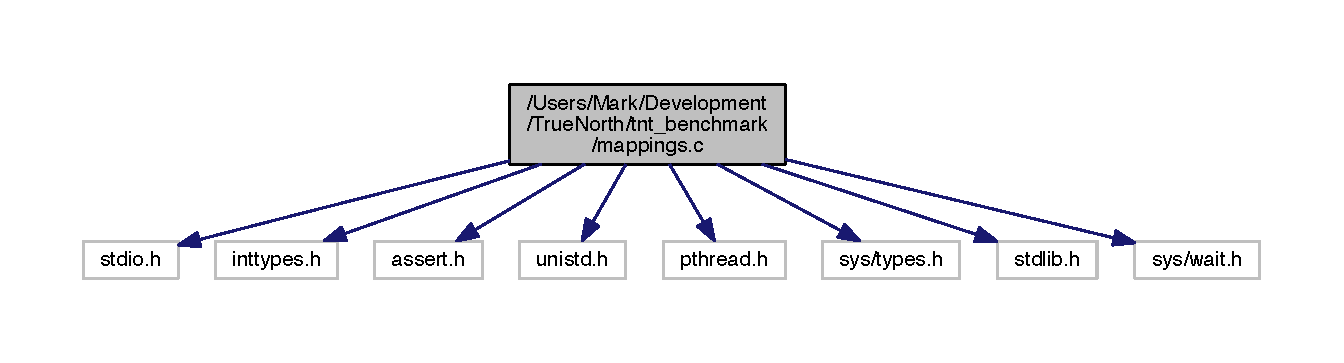
\includegraphics[width=350pt]{mappings_8c__incl}
\end{center}
\end{figure}
\subsection*{Macros}
\begin{DoxyCompactItemize}
\item 
\#define \hyperlink{mappings_8c_adc0d1d400308f82e4d42245c2fd946b9}{\+\_\+id\+Type}~int\+\_\+fast16\+\_\+t
\item 
\#define \hyperlink{mappings_8c_a368ddcd71f7b61cb0f918f22d07ce999}{\+\_\+ne\+Volt\+Type}~uint\+\_\+fast32\+\_\+t
\item 
\#define \hyperlink{mappings_8c_a7dd2b02e8e5ddb7f5b243002830d964f}{\+\_\+ne\+Stat\+Type}~int\+\_\+fast32\+\_\+t
\item 
\#define \hyperlink{mappings_8c_ac35d555a6883d7624a8fc918f6cc91c0}{regid\+\_\+t}~uint32\+\_\+t
\item 
\#define \hyperlink{mappings_8c_a672b405f17d1859fc9e26f09afe9a366}{gid\+\_\+t}~uint64\+\_\+t
\item 
\#define \hyperlink{mappings_8c_a83bb0fed7e64e381d564a9f1cb951fac}{L\+O\+C}(a)~((\hyperlink{mappings_8c_ac35d555a6883d7624a8fc918f6cc91c0}{regid\+\_\+t})a)
\item 
\#define \hyperlink{mappings_8c_a5bf12e6001846798b26182c47c53df9b}{C\+O\+R\+E}(a)~((\hyperlink{mappings_8c_ac35d555a6883d7624a8fc918f6cc91c0}{regid\+\_\+t})(((\hyperlink{mappings_8c_a672b405f17d1859fc9e26f09afe9a366}{gid\+\_\+t})(a) $>$$>$ 32) \& 0x\+F\+F\+F\+F\+F\+F\+F\+F))
\end{DoxyCompactItemize}
\subsection*{Functions}
\begin{DoxyCompactItemize}
\item 
void \hyperlink{mappings_8c_a37439d03a72ad06efda28e7783dcc958}{get\+Local\+I\+Ds} (\hyperlink{mappings_8c_a672b405f17d1859fc9e26f09afe9a366}{gid\+\_\+t} global, \hyperlink{mappings_8c_ac35d555a6883d7624a8fc918f6cc91c0}{regid\+\_\+t} $\ast$core, \hyperlink{mappings_8c_ac35d555a6883d7624a8fc918f6cc91c0}{regid\+\_\+t} $\ast$local)
\begin{DoxyCompactList}\small\item\em Given a global I\+D, return the core number. \end{DoxyCompactList}\item 
\hyperlink{mappings_8c_a672b405f17d1859fc9e26f09afe9a366}{gid\+\_\+t} \hyperlink{mappings_8c_aba4107cb441dd8f8732f72c359a691c4}{global\+I\+D} (\hyperlink{mappings_8c_ac35d555a6883d7624a8fc918f6cc91c0}{regid\+\_\+t} core, \hyperlink{mappings_8c_ac35d555a6883d7624a8fc918f6cc91c0}{regid\+\_\+t} local)
\item 
void $\ast$ \hyperlink{mappings_8c_a2fc3ede1a6cdf2b653f9d90c5f3c0a17}{test\+Val} (void $\ast$str)
\item 
int \hyperlink{mappings_8c_ae66f6b31b5ad750f1fe042a706a4e3d4}{main} ()
\end{DoxyCompactItemize}
\subsection*{Variables}
\begin{DoxyCompactItemize}
\item 
int \hyperlink{mappings_8c_a1d9155c121a82499c347e531f8ebc0ac}{numth} = 256
\item 
int \hyperlink{mappings_8c_ada3910bb0ed37969bc5a1e366028c53f}{cur} = 0
\item 
int \hyperlink{mappings_8c_ae1e1dde676c120fa6d10f3bb2c14059e}{max} = 16777215
\item 
int \hyperlink{mappings_8c_a44dd54637529327772a8ba08ab8e49b1}{per\+Th}
\end{DoxyCompactItemize}


\subsection{Macro Definition Documentation}
\hypertarget{mappings_8c_adc0d1d400308f82e4d42245c2fd946b9}{}\index{mappings.\+c@{mappings.\+c}!\+\_\+id\+Type@{\+\_\+id\+Type}}
\index{\+\_\+id\+Type@{\+\_\+id\+Type}!mappings.\+c@{mappings.\+c}}
\subsubsection[{\+\_\+id\+Type}]{\setlength{\rightskip}{0pt plus 5cm}\#define \+\_\+id\+Type~int\+\_\+fast16\+\_\+t}\label{mappings_8c_adc0d1d400308f82e4d42245c2fd946b9}


Definition at line 9 of file mappings.\+c.

\hypertarget{mappings_8c_a7dd2b02e8e5ddb7f5b243002830d964f}{}\index{mappings.\+c@{mappings.\+c}!\+\_\+ne\+Stat\+Type@{\+\_\+ne\+Stat\+Type}}
\index{\+\_\+ne\+Stat\+Type@{\+\_\+ne\+Stat\+Type}!mappings.\+c@{mappings.\+c}}
\subsubsection[{\+\_\+ne\+Stat\+Type}]{\setlength{\rightskip}{0pt plus 5cm}\#define \+\_\+ne\+Stat\+Type~int\+\_\+fast32\+\_\+t}\label{mappings_8c_a7dd2b02e8e5ddb7f5b243002830d964f}


Definition at line 12 of file mappings.\+c.

\hypertarget{mappings_8c_a368ddcd71f7b61cb0f918f22d07ce999}{}\index{mappings.\+c@{mappings.\+c}!\+\_\+ne\+Volt\+Type@{\+\_\+ne\+Volt\+Type}}
\index{\+\_\+ne\+Volt\+Type@{\+\_\+ne\+Volt\+Type}!mappings.\+c@{mappings.\+c}}
\subsubsection[{\+\_\+ne\+Volt\+Type}]{\setlength{\rightskip}{0pt plus 5cm}\#define \+\_\+ne\+Volt\+Type~uint\+\_\+fast32\+\_\+t}\label{mappings_8c_a368ddcd71f7b61cb0f918f22d07ce999}


Definition at line 11 of file mappings.\+c.

\hypertarget{mappings_8c_a5bf12e6001846798b26182c47c53df9b}{}\index{mappings.\+c@{mappings.\+c}!C\+O\+R\+E@{C\+O\+R\+E}}
\index{C\+O\+R\+E@{C\+O\+R\+E}!mappings.\+c@{mappings.\+c}}
\subsubsection[{C\+O\+R\+E}]{\setlength{\rightskip}{0pt plus 5cm}\#define C\+O\+R\+E(
\begin{DoxyParamCaption}
\item[{}]{a}
\end{DoxyParamCaption}
)~(({\bf regid\+\_\+t})((({\bf gid\+\_\+t})(a) $>$$>$ 32) \& 0x\+F\+F\+F\+F\+F\+F\+F\+F))}\label{mappings_8c_a5bf12e6001846798b26182c47c53df9b}


Definition at line 18 of file mappings.\+c.

\hypertarget{mappings_8c_a672b405f17d1859fc9e26f09afe9a366}{}\index{mappings.\+c@{mappings.\+c}!gid\+\_\+t@{gid\+\_\+t}}
\index{gid\+\_\+t@{gid\+\_\+t}!mappings.\+c@{mappings.\+c}}
\subsubsection[{gid\+\_\+t}]{\setlength{\rightskip}{0pt plus 5cm}\#define gid\+\_\+t~uint64\+\_\+t}\label{mappings_8c_a672b405f17d1859fc9e26f09afe9a366}


Definition at line 14 of file mappings.\+c.

\hypertarget{mappings_8c_a83bb0fed7e64e381d564a9f1cb951fac}{}\index{mappings.\+c@{mappings.\+c}!L\+O\+C@{L\+O\+C}}
\index{L\+O\+C@{L\+O\+C}!mappings.\+c@{mappings.\+c}}
\subsubsection[{L\+O\+C}]{\setlength{\rightskip}{0pt plus 5cm}\#define L\+O\+C(
\begin{DoxyParamCaption}
\item[{}]{a}
\end{DoxyParamCaption}
)~(({\bf regid\+\_\+t})a)}\label{mappings_8c_a83bb0fed7e64e381d564a9f1cb951fac}


Definition at line 17 of file mappings.\+c.

\hypertarget{mappings_8c_ac35d555a6883d7624a8fc918f6cc91c0}{}\index{mappings.\+c@{mappings.\+c}!regid\+\_\+t@{regid\+\_\+t}}
\index{regid\+\_\+t@{regid\+\_\+t}!mappings.\+c@{mappings.\+c}}
\subsubsection[{regid\+\_\+t}]{\setlength{\rightskip}{0pt plus 5cm}\#define regid\+\_\+t~uint32\+\_\+t}\label{mappings_8c_ac35d555a6883d7624a8fc918f6cc91c0}


Definition at line 13 of file mappings.\+c.



\subsection{Function Documentation}
\hypertarget{mappings_8c_a37439d03a72ad06efda28e7783dcc958}{}\index{mappings.\+c@{mappings.\+c}!get\+Local\+I\+Ds@{get\+Local\+I\+Ds}}
\index{get\+Local\+I\+Ds@{get\+Local\+I\+Ds}!mappings.\+c@{mappings.\+c}}
\subsubsection[{get\+Local\+I\+Ds}]{\setlength{\rightskip}{0pt plus 5cm}void get\+Local\+I\+Ds (
\begin{DoxyParamCaption}
\item[{{\bf gid\+\_\+t}}]{global, }
\item[{{\bf regid\+\_\+t} $\ast$}]{core, }
\item[{{\bf regid\+\_\+t} $\ast$}]{local}
\end{DoxyParamCaption}
)}\label{mappings_8c_a37439d03a72ad06efda28e7783dcc958}


Given a global I\+D, return the core number. 



Definition at line 22 of file mappings.\+c.



Referenced by test\+Val().


\begin{DoxyCode}
22                                                                \{
23     (*core) = \hyperlink{mappings_8c_a5bf12e6001846798b26182c47c53df9b}{CORE}(global);
24     (*local)= \hyperlink{mappings_8c_a83bb0fed7e64e381d564a9f1cb951fac}{LOC}(global);
25 \}
\end{DoxyCode}
\hypertarget{mappings_8c_aba4107cb441dd8f8732f72c359a691c4}{}\index{mappings.\+c@{mappings.\+c}!global\+I\+D@{global\+I\+D}}
\index{global\+I\+D@{global\+I\+D}!mappings.\+c@{mappings.\+c}}
\subsubsection[{global\+I\+D}]{\setlength{\rightskip}{0pt plus 5cm}{\bf gid\+\_\+t} global\+I\+D (
\begin{DoxyParamCaption}
\item[{{\bf regid\+\_\+t}}]{core, }
\item[{{\bf regid\+\_\+t}}]{local}
\end{DoxyParamCaption}
)}\label{mappings_8c_aba4107cb441dd8f8732f72c359a691c4}


Definition at line 26 of file mappings.\+c.


\begin{DoxyCode}
26                                            \{
27     \hyperlink{mappings_8c_a672b405f17d1859fc9e26f09afe9a366}{gid\_t} returnVal = 0;
28     returnVal = ((uint64\_t)core << 32) | local;
29     \textcolor{keywordflow}{return} returnVal;
30 \}
\end{DoxyCode}
\hypertarget{mappings_8c_ae66f6b31b5ad750f1fe042a706a4e3d4}{}\index{mappings.\+c@{mappings.\+c}!main@{main}}
\index{main@{main}!mappings.\+c@{mappings.\+c}}
\subsubsection[{main}]{\setlength{\rightskip}{0pt plus 5cm}int main (
\begin{DoxyParamCaption}
{}
\end{DoxyParamCaption}
)}\label{mappings_8c_ae66f6b31b5ad750f1fe042a706a4e3d4}


Definition at line 97 of file mappings.\+c.



References global\+I\+D(), max, numth, per\+Th, and test\+Val().


\begin{DoxyCode}
97            \{
98     printf(\textcolor{stringliteral}{"Enter."});
99     printf(\textcolor{stringliteral}{"running tests.\(\backslash\)n"});
100 
101 
102 
103     \hyperlink{mappings_8c_a672b405f17d1859fc9e26f09afe9a366}{gid\_t} global;
104     \hyperlink{mappings_8c_ac35d555a6883d7624a8fc918f6cc91c0}{regid\_t} core = 72000;
105 
106     \hyperlink{mappings_8c_ac35d555a6883d7624a8fc918f6cc91c0}{regid\_t} local = 0;
107     global = \hyperlink{mappings_8c_aba4107cb441dd8f8732f72c359a691c4}{globalID}(core,local);
108     \hyperlink{mappings_8c_a672b405f17d1859fc9e26f09afe9a366}{gid\_t} g2 = global;
109     printf(\textcolor{stringliteral}{"Core is :%u\(\backslash\)n\(\backslash\)n\(\backslash\)n"},\hyperlink{mappings_8c_a5bf12e6001846798b26182c47c53df9b}{CORE}(global));
110 
111 
112 
113 
114 
115 
116 
117     dup2(STDOUT\_FILENO, STDERR\_FILENO);
118     \textcolor{keywordtype}{int} status;
119     \textcolor{comment}{//pid\_t p = fork();}
120 
121     \hyperlink{mappings_8c_a44dd54637529327772a8ba08ab8e49b1}{perTh} = \hyperlink{mappings_8c_ae1e1dde676c120fa6d10f3bb2c14059e}{max}/\hyperlink{mappings_8c_a1d9155c121a82499c347e531f8ebc0ac}{numth};
122     pthread\_t threads[\hyperlink{mappings_8c_a1d9155c121a82499c347e531f8ebc0ac}{numth}];
123     \textcolor{keywordtype}{long} * thread\_args[\hyperlink{mappings_8c_a1d9155c121a82499c347e531f8ebc0ac}{numth}];
124     \textcolor{keywordtype}{int} result\_code;
125     \textcolor{keywordtype}{int} currentSearchVal = 0;
126     \textcolor{keywordflow}{for}(\textcolor{keywordtype}{int} i = 0; i  < \hyperlink{mappings_8c_a1d9155c121a82499c347e531f8ebc0ac}{numth}; i ++)\{
127 
128         thread\_args[i] = (\textcolor{keywordtype}{long} *) malloc (\textcolor{keyword}{sizeof}(\textcolor{keywordtype}{long}));
129         *thread\_args[i] = i;
130           printf(\textcolor{stringliteral}{"main - creating thread %i with max search index of %i\(\backslash\)n"},i,*thread\_args[i]);
131         result\_code = pthread\_create(&threads[i], NULL, \hyperlink{mappings_8c_a2fc3ede1a6cdf2b653f9d90c5f3c0a17}{testVal}, (\textcolor{keywordtype}{void}*) thread\_args[i]);
132     \}
133 
134 
135     \textcolor{comment}{/*}
136 \textcolor{comment}{    for(int i = 0; i < 100000; i++)}
137 \textcolor{comment}{    \{}
138 \textcolor{comment}{        for(int j = 0; j < 100000; j++)}
139 \textcolor{comment}{        \{}
140 \textcolor{comment}{            regid\_t core = i;}
141 \textcolor{comment}{            regid\_t local = j;}
142 \textcolor{comment}{            gid\_t global = globalID(core,local);}
143 \textcolor{comment}{            assert(i == core);}
144 \textcolor{comment}{            assert(j == local);}
145 \textcolor{comment}{}
146 \textcolor{comment}{            core = CORE(global);}
147 \textcolor{comment}{            local = LOC(local);}
148 \textcolor{comment}{            assert(core == i);}
149 \textcolor{comment}{            assert(local == j);}
150 \textcolor{comment}{}
151 \textcolor{comment}{            getLocalIDs(global, &core, &local);}
152 \textcolor{comment}{            assert(core == i);}
153 \textcolor{comment}{            assert(local ==j);}
154 \textcolor{comment}{}
155 \textcolor{comment}{        \}}
156 \textcolor{comment}{    \}*/}
157     \textcolor{keywordflow}{for} (\textcolor{keywordtype}{int} index = 0; index < \hyperlink{mappings_8c_a1d9155c121a82499c347e531f8ebc0ac}{numth}; ++index) \{
158         \textcolor{comment}{// block until thread 'index' completes}
159         result\_code = pthread\_join(threads[index], NULL);
160         printf(\textcolor{stringliteral}{"In main: thread %d has completed\(\backslash\)n"}, index);
161         assert(0 == result\_code);
162     \}
163 
164     dup2(STDERR\_FILENO,STDOUT\_FILENO);
165     \textcolor{keywordtype}{int} w;
166     \textcolor{comment}{//if(p != 0 )}
167     \textcolor{comment}{//  w = waitpid(p, &status, WUNTRACED | WCONTINUED);}
168     printf(\textcolor{stringliteral}{"Testing complete.\(\backslash\)n"});
169 
170     \}
\end{DoxyCode}


Here is the call graph for this function\+:\nopagebreak
\begin{figure}[H]
\begin{center}
\leavevmode
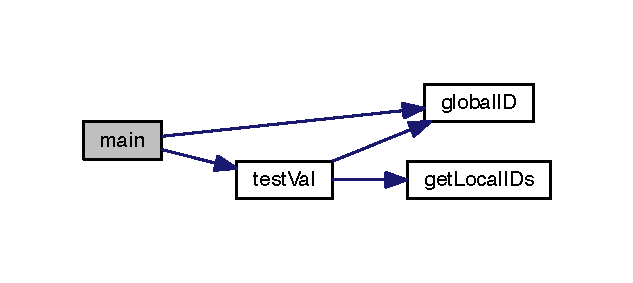
\includegraphics[width=304pt]{mappings_8c_ae66f6b31b5ad750f1fe042a706a4e3d4_cgraph}
\end{center}
\end{figure}


\hypertarget{mappings_8c_a2fc3ede1a6cdf2b653f9d90c5f3c0a17}{}\index{mappings.\+c@{mappings.\+c}!test\+Val@{test\+Val}}
\index{test\+Val@{test\+Val}!mappings.\+c@{mappings.\+c}}
\subsubsection[{test\+Val}]{\setlength{\rightskip}{0pt plus 5cm}void$\ast$ test\+Val (
\begin{DoxyParamCaption}
\item[{void $\ast$}]{str}
\end{DoxyParamCaption}
)}\label{mappings_8c_a2fc3ede1a6cdf2b653f9d90c5f3c0a17}


Definition at line 36 of file mappings.\+c.



References get\+Local\+I\+Ds(), global\+I\+D(), and max.



Referenced by main().


\begin{DoxyCode}
36                           \{
37     \textcolor{keywordtype}{long} starti =(*(\textcolor{keywordtype}{long} *)  str ) * \hyperlink{mappings_8c_ae1e1dde676c120fa6d10f3bb2c14059e}{max};
38     \textcolor{keywordtype}{long} startj = startj;
39     \textcolor{keywordtype}{long} endj= starti + \hyperlink{mappings_8c_ae1e1dde676c120fa6d10f3bb2c14059e}{max};
40     \textcolor{keywordtype}{long} endi = endj;
41     \textcolor{comment}{//printf("Thread checking in with start at %i and end at %i.\(\backslash\)n", starti, endi);}
42     \textcolor{keywordflow}{for}(\textcolor{keywordtype}{long} i = starti; i < endi; i ++)
43     \{
44         \textcolor{keywordflow}{for}(\textcolor{keywordtype}{long} j = startj; j <endj; j++)\{
45             \hyperlink{mappings_8c_ac35d555a6883d7624a8fc918f6cc91c0}{regid\_t} core = i;
46             \hyperlink{mappings_8c_ac35d555a6883d7624a8fc918f6cc91c0}{regid\_t} local = j;
47             \hyperlink{mappings_8c_a672b405f17d1859fc9e26f09afe9a366}{gid\_t} global = \hyperlink{mappings_8c_aba4107cb441dd8f8732f72c359a691c4}{globalID}(core,local);
48 
49             core = \hyperlink{mappings_8c_a5bf12e6001846798b26182c47c53df9b}{CORE}(global);
50             local = \hyperlink{mappings_8c_a83bb0fed7e64e381d564a9f1cb951fac}{LOC}(local);
51             \textcolor{keywordflow}{if}(core != i)
52             \{
53                 \textcolor{comment}{//ec 1:}
54                 printf(\textcolor{stringliteral}{"\(\backslash\)n*******************************Manual Dump CORE **************************\(\backslash\)n "}
55                                \textcolor{stringliteral}{"Core was %u, should have been %li - first check fail, line 57 -- \(\backslash\)n"}
56                                \textcolor{stringliteral}{"Local was %u should have been %li\(\backslash\)n"}
57                                \textcolor{stringliteral}{"\(\backslash\)t-------*****************---\(\backslash\)t"}, core, i,local,j);
58             \}
59             \textcolor{keywordflow}{if}(local != j)
60             \{
61                 \textcolor{comment}{//ec 2:}
62                 printf(\textcolor{stringliteral}{"\(\backslash\)n*******************************Manual Dump LOCAL**************************\(\backslash\)n "}
63                                \textcolor{stringliteral}{"Core was %u, should have been %li - first check fail, line 63. -- \(\backslash\)n"}
64                                \textcolor{stringliteral}{"Local was %u, should have been %li\(\backslash\)n"}
65                                \textcolor{stringliteral}{"\(\backslash\)t-------*****************---\(\backslash\)t"}, core, i,local,j);
66             \}
67             \textcolor{comment}{//assert(core == i);}
68             \textcolor{comment}{//assert(local == j);}
69 
70             \hyperlink{mappings_8c_a37439d03a72ad06efda28e7783dcc958}{getLocalIDs}(global, &core, &local);
71             \textcolor{keywordflow}{if}(core != i)
72             \{
73                 \textcolor{comment}{//ec 1:}
74                 printf(\textcolor{stringliteral}{"\(\backslash\)n*******************************Manual Dump CORE**************************\(\backslash\)n "}
75                                \textcolor{stringliteral}{"Core was %u, should have been %li - second check fail, line 73 -- \(\backslash\)n"}
76                                \textcolor{stringliteral}{"Local was %u, should have been %li\(\backslash\)n"}
77                                \textcolor{stringliteral}{"\(\backslash\)t-------*****************---\(\backslash\)t"}, core, i,local,j);
78             \}
79             \textcolor{keywordflow}{if}(local != j)
80             \{
81                 \textcolor{comment}{//ec 2:}
82                 printf(\textcolor{stringliteral}{"\(\backslash\)n*******************************Manual Dump LOCAL**************************\(\backslash\)n "}
83                                \textcolor{stringliteral}{"Core was %u, should have been %li - first check fail, line 63. -- \(\backslash\)n"}
84                                \textcolor{stringliteral}{"Local was %u, should have been %li\(\backslash\)n"}
85                                \textcolor{stringliteral}{"\(\backslash\)t-------*****************---\(\backslash\)t"}, core, i,local,j);
86 
87             \}
88             assert(core == i);
89             assert(local ==j);
90 
91         \}
92     \}
93 
94     \textcolor{keywordflow}{return} NULL;
95 \}
\end{DoxyCode}


Here is the call graph for this function\+:\nopagebreak
\begin{figure}[H]
\begin{center}
\leavevmode
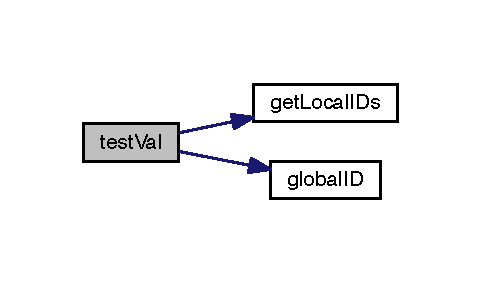
\includegraphics[width=231pt]{mappings_8c_a2fc3ede1a6cdf2b653f9d90c5f3c0a17_cgraph}
\end{center}
\end{figure}




\subsection{Variable Documentation}
\hypertarget{mappings_8c_ada3910bb0ed37969bc5a1e366028c53f}{}\index{mappings.\+c@{mappings.\+c}!cur@{cur}}
\index{cur@{cur}!mappings.\+c@{mappings.\+c}}
\subsubsection[{cur}]{\setlength{\rightskip}{0pt plus 5cm}int cur = 0}\label{mappings_8c_ada3910bb0ed37969bc5a1e366028c53f}


Definition at line 32 of file mappings.\+c.

\hypertarget{mappings_8c_ae1e1dde676c120fa6d10f3bb2c14059e}{}\index{mappings.\+c@{mappings.\+c}!max@{max}}
\index{max@{max}!mappings.\+c@{mappings.\+c}}
\subsubsection[{max}]{\setlength{\rightskip}{0pt plus 5cm}int max = 16777215}\label{mappings_8c_ae1e1dde676c120fa6d10f3bb2c14059e}


Definition at line 33 of file mappings.\+c.



Referenced by main(), and test\+Val().

\hypertarget{mappings_8c_a1d9155c121a82499c347e531f8ebc0ac}{}\index{mappings.\+c@{mappings.\+c}!numth@{numth}}
\index{numth@{numth}!mappings.\+c@{mappings.\+c}}
\subsubsection[{numth}]{\setlength{\rightskip}{0pt plus 5cm}int numth = 256}\label{mappings_8c_a1d9155c121a82499c347e531f8ebc0ac}


Definition at line 31 of file mappings.\+c.



Referenced by main().

\hypertarget{mappings_8c_a44dd54637529327772a8ba08ab8e49b1}{}\index{mappings.\+c@{mappings.\+c}!per\+Th@{per\+Th}}
\index{per\+Th@{per\+Th}!mappings.\+c@{mappings.\+c}}
\subsubsection[{per\+Th}]{\setlength{\rightskip}{0pt plus 5cm}int per\+Th}\label{mappings_8c_a44dd54637529327772a8ba08ab8e49b1}


Definition at line 34 of file mappings.\+c.



Referenced by main().


\hypertarget{model__main_8c}{}\section{/\+Users/\+Mark/\+Development/\+True\+North/tnt\+\_\+benchmark/model\+\_\+main.c File Reference}
\label{model__main_8c}\index{/\+Users/\+Mark/\+Development/\+True\+North/tnt\+\_\+benchmark/model\+\_\+main.\+c@{/\+Users/\+Mark/\+Development/\+True\+North/tnt\+\_\+benchmark/model\+\_\+main.\+c}}
{\ttfamily \#include \char`\"{}model\+\_\+main.\+h\char`\"{}}\\*
Include dependency graph for model\+\_\+main.\+c\+:\nopagebreak
\begin{figure}[H]
\begin{center}
\leavevmode
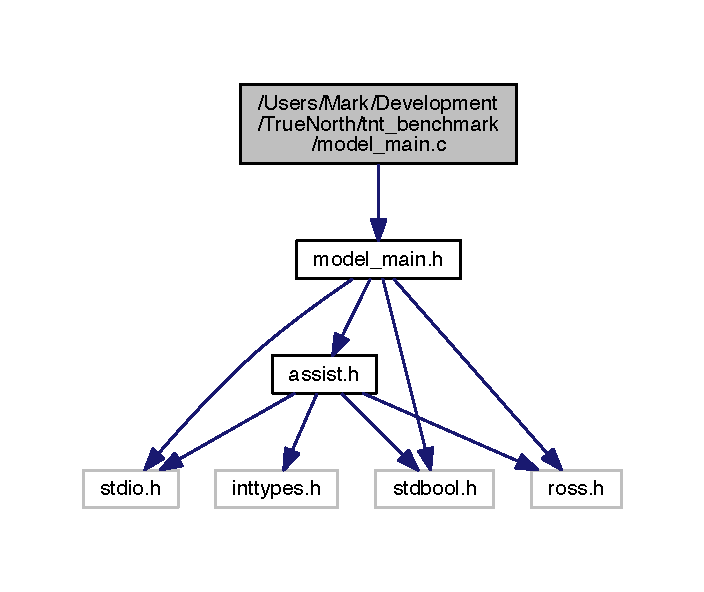
\includegraphics[width=338pt]{model__main_8c__incl}
\end{center}
\end{figure}
\subsection*{Functions}
\begin{DoxyCompactItemize}
\item 
int \hyperlink{model__main_8c_ae66f6b31b5ad750f1fe042a706a4e3d4}{main} ()
\end{DoxyCompactItemize}


\subsection{Function Documentation}
\hypertarget{model__main_8c_ae66f6b31b5ad750f1fe042a706a4e3d4}{}\index{model\+\_\+main.\+c@{model\+\_\+main.\+c}!main@{main}}
\index{main@{main}!model\+\_\+main.\+c@{model\+\_\+main.\+c}}
\subsubsection[{main}]{\setlength{\rightskip}{0pt plus 5cm}int main (
\begin{DoxyParamCaption}
{}
\end{DoxyParamCaption}
)}\label{model__main_8c_ae66f6b31b5ad750f1fe042a706a4e3d4}


Definition at line \hyperlink{model__main_8c_source_l00011}{11} of file \hyperlink{model__main_8c_source}{model\+\_\+main.\+c}.


\begin{DoxyCode}
00011            \{
00012     \textcolor{keywordflow}{return} 0;
00013 \}
\end{DoxyCode}

\hypertarget{model__main_8h}{}\section{/\+Users/\+Mark/\+Development/\+True\+North/tnt\+\_\+benchmark/model\+\_\+main.h File Reference}
\label{model__main_8h}\index{/\+Users/\+Mark/\+Development/\+True\+North/tnt\+\_\+benchmark/model\+\_\+main.\+h@{/\+Users/\+Mark/\+Development/\+True\+North/tnt\+\_\+benchmark/model\+\_\+main.\+h}}
{\ttfamily \#include \char`\"{}models/neuron\+\_\+model.\+h\char`\"{}}\\*
{\ttfamily \#include \char`\"{}models/synapse.\+h\char`\"{}}\\*
{\ttfamily \#include \char`\"{}assist.\+h\char`\"{}}\\*
{\ttfamily \#include \char`\"{}ross.\+h\char`\"{}}\\*
{\ttfamily \#include \char`\"{}spike\+\_\+generator.\+h\char`\"{}}\\*
{\ttfamily \#include \char`\"{}libs/sqlite3.\+h\char`\"{}}\\*
{\ttfamily \#include $<$stdio.\+h$>$}\\*
Include dependency graph for model\+\_\+main.\+h\+:\nopagebreak
\begin{figure}[H]
\begin{center}
\leavevmode
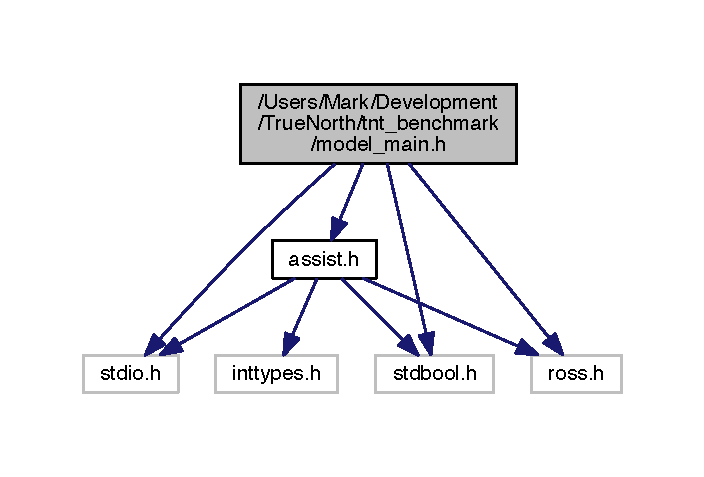
\includegraphics[width=350pt]{model__main_8h__incl}
\end{center}
\end{figure}
This graph shows which files directly or indirectly include this file\+:\nopagebreak
\begin{figure}[H]
\begin{center}
\leavevmode
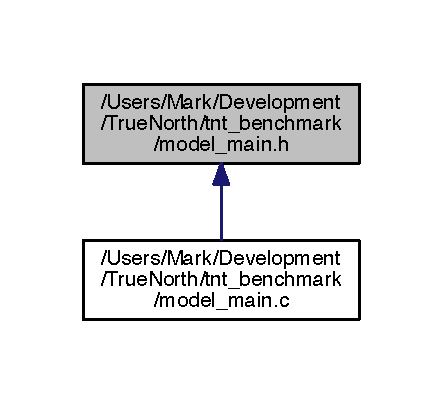
\includegraphics[width=212pt]{model__main_8h__dep__incl}
\end{center}
\end{figure}
\subsection*{Functions}
\begin{DoxyCompactItemize}
\item 
void \hyperlink{model__main_8h_a7a8df3f99e1d582c6c136b16d6e34d13}{pre\+\_\+run} ()
\item 
void \hyperlink{model__main_8h_a9309446aa05714b141a3d3caae4254db}{neuron\+\_\+event} (\hyperlink{structneuron_state}{neuron\+State} $\ast$s, tw\+\_\+bf $\ast$C\+V, \hyperlink{struct_msg___data}{Msg\+\_\+\+Data} $\ast$M, tw\+\_\+lp $\ast$lp)
\item 
void \hyperlink{model__main_8h_aea7de5bc5028e2df35cf3fe64f6cca6c}{synapse\+\_\+event} (\hyperlink{structsynapse_state}{synapse\+State} $\ast$s, tw\+\_\+bf $\ast$, \hyperlink{struct_msg___data}{Msg\+\_\+\+Data} $\ast$M, tw\+\_\+lp $\ast$lp)
\item 
void \hyperlink{model__main_8h_a8022723eba89664cca80e179b80a2b37}{neuron\+\_\+init} (\hyperlink{structneuron_state}{neuron\+State} $\ast$s, tw\+\_\+lp $\ast$lp)
\item 
void \hyperlink{model__main_8h_a579d8e5af0b1c0a80c8e83b7a534f873}{synapse\+\_\+init} (\hyperlink{structsynapse_state}{synapse\+State} $\ast$s, tw\+\_\+lp $\ast$lp)
\item 
void \hyperlink{model__main_8h_a801f93205937969fea2eff0bf2e76de9}{set\+Synapse\+Weight} (\hyperlink{structneuron_state}{neuron\+State} $\ast$s, tw\+\_\+lp $\ast$lp, int synapse\+I\+D)
\item 
void \hyperlink{model__main_8h_a4bd8bcd9c6de148a9f5c84fadd51106c}{neuron\+\_\+reverse} (\hyperlink{structneuron_state}{neuron\+State} $\ast$, tw\+\_\+bf $\ast$, \hyperlink{struct_msg___data}{Msg\+\_\+\+Data} $\ast$, tw\+\_\+lp $\ast$)
\item 
void \hyperlink{model__main_8h_a36fba0f7780630192391905fb40470cc}{synapse\+\_\+reverse} (\hyperlink{structneuron_state}{neuron\+State} $\ast$, tw\+\_\+bf $\ast$, \hyperlink{struct_msg___data}{Msg\+\_\+\+Data} $\ast$, tw\+\_\+lp $\ast$)
\item 
void \hyperlink{model__main_8h_a1f668d7246282bb6f62de09f934bee56}{synapse\+In} (int synapse\+I\+D, \hyperlink{structneuron_state}{neuron\+State} $\ast$s)
\item 
void \hyperlink{model__main_8h_a3b6bb8c3f517cbc71b3a12379f286c7f}{calculate\+Threshold} (int synapse\+I\+D, \hyperlink{structneuron_state}{neuron\+State} $\ast$s)
\item 
void \hyperlink{model__main_8h_ad3022d255395cdd5ce59a7a210232805}{check\+Fire} (int synapse\+I\+D, \hyperlink{structneuron_state}{neuron\+State} $\ast$s)
\item 
void \hyperlink{model__main_8h_acac9e41bea7d1d0911a0220de60a37b0}{neuron\+\_\+final} (\hyperlink{structneuron_state}{neuron\+State} $\ast$s, tw\+\_\+lp $\ast$lp)
\item 
void \hyperlink{model__main_8h_a3d695e7995cce87a03d6407d801e043d}{synapse\+\_\+final} (\hyperlink{structsynapse_state}{synapse\+State} $\ast$s, tw\+\_\+lp $\ast$lp)
\item 
void \hyperlink{model__main_8h_a90307b42f2863f00eb0d4290e576e0d2}{gen\+\_\+init} (\hyperlink{structspike_gen_state}{spike\+Gen\+State} $\ast$gen\+\_\+state, tw\+\_\+lp $\ast$lp)
\item 
void \hyperlink{model__main_8h_a9f6f8d34d84c91c98139da79b73a5996}{gen\+\_\+pre} (\hyperlink{structspike_gen_state}{spike\+Gen\+State} $\ast$gen\+\_\+state, tw\+\_\+lp $\ast$lp)
\item 
void \hyperlink{model__main_8h_a9b676e87fee87da0053e1af467a663da}{gen\+\_\+event} (\hyperlink{structspike_gen_state}{spike\+Gen\+State} $\ast$gen\+\_\+state, tw\+\_\+lp $\ast$lp)
\item 
void \hyperlink{model__main_8h_a655eec05ddf277450c550f96853a9799}{gen\+\_\+reverse} (\hyperlink{structspike_gen_state}{spike\+Gen\+State} $\ast$gen\+\_\+state, tw\+\_\+lp $\ast$lp)
\item 
void \hyperlink{model__main_8h_a8d028b3e829d2f44994be14d1cdcf84b}{gen\+\_\+final} (\hyperlink{structspike_gen_state}{spike\+Gen\+State} $\ast$gen\+\_\+state, tw\+\_\+lp $\ast$lp)
\item 
void \hyperlink{model__main_8h_a37439d03a72ad06efda28e7783dcc958}{get\+Local\+I\+Ds} (\hyperlink{mappings_8c_a672b405f17d1859fc9e26f09afe9a366}{gid\+\_\+t} global, \hyperlink{mappings_8c_ac35d555a6883d7624a8fc918f6cc91c0}{regid\+\_\+t} $\ast$core, \hyperlink{mappings_8c_ac35d555a6883d7624a8fc918f6cc91c0}{regid\+\_\+t} $\ast$local)
\begin{DoxyCompactList}\small\item\em Given a global I\+D, return the core number. \end{DoxyCompactList}\item 
\hyperlink{mappings_8c_a672b405f17d1859fc9e26f09afe9a366}{gid\+\_\+t} \hyperlink{model__main_8h_aba4107cb441dd8f8732f72c359a691c4}{global\+I\+D} (\hyperlink{mappings_8c_ac35d555a6883d7624a8fc918f6cc91c0}{regid\+\_\+t} core, \hyperlink{mappings_8c_ac35d555a6883d7624a8fc918f6cc91c0}{regid\+\_\+t} local)
\item 
void \hyperlink{model__main_8h_aa30d3f27017c4332fce3dca3ce944a67}{init\+Random\+Wts} (\hyperlink{structneuron_state}{neuron\+State} $\ast$s, tw\+\_\+lp $\ast$lp)
\begin{DoxyCompactList}\small\item\em neuron init helper functions\+: \end{DoxyCompactList}\item 
void \hyperlink{model__main_8h_aca6527a1ad95c75e8a0ba7d0b30b49fb}{init\+Random\+Recurrance} (\hyperlink{structneuron_state}{neuron\+State} $\ast$s)
\item 
void \hyperlink{model__main_8h_a4d92cef623a227e757b28c6068cf806c}{set\+Neuron\+Threshold} (\hyperlink{structneuron_state}{neuron\+State} $\ast$s, tw\+\_\+lp $\ast$lp)
\begin{DoxyCompactList}\small\item\em set\+Neuron\+Threshold -\/ Sets the threshold value of the neuron. \end{DoxyCompactList}\item 
void \hyperlink{model__main_8h_adb8d460fbe64ef0fdeb18a822e4e17fa}{init\+Neruon\+With\+Map} (\hyperlink{structneuron_state}{neuron\+State} $\ast$s, tw\+\_\+lp $\ast$lp, tw\+\_\+pe $\ast$pe)
\item 
void \hyperlink{model__main_8h_a1c2ffbc27679a309adf4732931990532}{init\+Synapse\+With\+Map} (\hyperlink{structneuron_state}{neuron\+State} $\ast$s, tw\+\_\+lp $\ast$lp, tw\+\_\+pe $\ast$pe)
\begin{DoxyCompactList}\small\item\em init\+Synapse\+With\+Map -- Initializes this particular synapse based on the sqllite map. \end{DoxyCompactList}\end{DoxyCompactItemize}
\subsection*{Variables}
\begin{DoxyCompactItemize}
\item 
int \hyperlink{model__main_8h_a67e8e45768f76b984a60fcff2b7c51aa}{N\+E\+U\+R\+O\+N\+S\+\_\+\+I\+N\+\_\+\+C\+O\+R\+E} = 4
\begin{DoxyCompactList}\small\item\em Number of neurons per core. \end{DoxyCompactList}\item 
int \hyperlink{model__main_8h_a076b99099b46431255982b2bb8ce06fb}{S\+Y\+N\+A\+P\+S\+E\+S\+\_\+\+I\+N\+\_\+\+C\+O\+R\+E} = 8
\begin{DoxyCompactList}\small\item\em Number of synapses per core. \end{DoxyCompactList}\item 
int \hyperlink{model__main_8h_a851557110b7442a40078d6ef85c2de76}{C\+O\+R\+E\+S\+\_\+\+P\+E\+R\+\_\+\+P\+E} = 2
\begin{DoxyCompactList}\small\item\em Each P\+E can have one or more virtual cores running during the simulation. \end{DoxyCompactList}\item 
int \hyperlink{model__main_8h_a433873baf41da436ba9c1734c8c5ddd2}{T\+H\+R\+E\+S\+H\+O\+L\+D\+\_\+\+M\+A\+X} = 11
\begin{DoxyCompactList}\small\item\em Determines the maximum and minimum thresholds for a neuron to fire. \end{DoxyCompactList}\item 
int \hyperlink{model__main_8h_a55f4484944f4174b5e677c0a71b30e4a}{T\+H\+R\+E\+S\+H\+O\+L\+D\+\_\+\+M\+I\+N} = 5
\begin{DoxyCompactList}\small\item\em Minimum threshold. \end{DoxyCompactList}\item 
int \hyperlink{model__main_8h_a20ef6d41d2f384358522fb59fb6226cb}{S\+Y\+N\+A\+P\+S\+E\+\_\+\+W\+E\+I\+G\+H\+T\+\_\+\+M\+A\+X} = 10
\begin{DoxyCompactList}\small\item\em Each neuron is connected to the synapses (inputs) within the core it is running in. \end{DoxyCompactList}\item 
int \hyperlink{model__main_8h_af38a0e2e2483ef81f7ea5175c366ce82}{S\+Y\+N\+A\+P\+S\+E\+\_\+\+W\+E\+I\+G\+H\+T\+\_\+\+M\+I\+N} = 5
\begin{DoxyCompactList}\small\item\em Minimum synapse weight. \end{DoxyCompactList}\item 
int \hyperlink{model__main_8h_ad39b86a0b748731175572436f6672264}{C\+O\+R\+E\+\_\+\+S\+I\+Z\+E}
\item 
float \hyperlink{model__main_8h_a0cd5ccf63b6dd9b12098d82503d03c05}{C\+L\+O\+C\+K\+\_\+\+S\+P\+E\+E\+D} = 1
\item 
int \hyperlink{model__main_8h_a8f579325f29e8089879da11747d83c96}{G\+E\+N\+\_\+\+L\+A\+G} = 1000
\item 
bool \hyperlink{model__main_8h_ac18d5985ff9fbfe912f1336eaa82ead6}{U\+S\+E\+\_\+\+O\+T\+H\+E\+R\+\_\+\+L\+E\+A\+K\+S} = false
\item 
bool \hyperlink{model__main_8h_a2a2a6154f99c6f9aa80e1afdcdc8d0d6}{U\+S\+E\+\_\+\+O\+T\+H\+E\+R\+\_\+\+R\+E\+S\+E\+T} = false
\item 
int \hyperlink{model__main_8h_abf39b7bc925f61737112787c578b06d3}{M\+I\+N\+\_\+\+L\+E\+A\+K} = 0
\item 
int \hyperlink{model__main_8h_a83c9373146a1150aa913c244e69abcaa}{M\+A\+X\+\_\+\+L\+E\+A\+K} = 10
\item 
char $\ast$ \hyperlink{model__main_8h_aa7b16932280ed0b12a0b4e7d675aac25}{A\+L\+T\+\_\+\+L\+E\+A\+K}
\item 
char $\ast$ \hyperlink{model__main_8h_a4c27ccb8c2f6992dcb9a961cc45e69a1}{A\+L\+T\+\_\+\+R\+E\+S\+E\+T}
\item 
int \hyperlink{model__main_8h_a789de05c7ed7a8cfadbd6b2e0c75516c}{M\+I\+N\+\_\+\+R\+E\+S\+E\+T} = 0
\item 
int \hyperlink{model__main_8h_ad6e4d5bfe16dc8db2633d5687661cfc8}{M\+A\+X\+\_\+\+R\+E\+S\+E\+T} = 10
\item 
int \hyperlink{model__main_8h_ac858bb435ac6b897dd949dbfdc61b5a5}{D\+E\+B\+U\+G\+\_\+\+M\+O\+D\+E} = 0
\item 
char $\ast$ \hyperlink{model__main_8h_a4e253d6390edbb51c63eac572d72b97a}{config\+File\+Path}
\item 
bool \hyperlink{model__main_8h_a002a2a64f4efdb283983d95f46f92596}{is\+File}
\item 
tw\+\_\+stime \hyperlink{model__main_8h_ac877337ae1e75d1b6640f41799f5a72c}{lookahead} = .\+00000000001
\item 
int \hyperlink{model__main_8h_a47d27feae0fedebece9a496a627122b9}{events\+\_\+per\+\_\+pe} = 0
\item 
int \hyperlink{model__main_8h_aaf6452b3f3c110587b95a22cf85b364a}{E\+X\+E\+C\+\_\+\+M\+E\+M\+O\+R\+Y} = 100000000
\item 
int \hyperlink{model__main_8h_a31c1ceb0e0910a3bc41f26c66252b321}{C\+L\+O\+C\+K\+\_\+\+R\+A\+T\+E} = 10
\item 
int \hyperlink{model__main_8h_aaa8f238cc23dfaa638510e226aad9df6}{tt\+\_\+neurons} = 0
\item 
int \hyperlink{model__main_8h_abb2a31424ba8aab7f54e79ae2cba5859}{tt\+\_\+synapses} = 0
\item 
bool \hyperlink{model__main_8h_ad65c1aa107c6fb135e0a75ecc78d52b2}{G\+E\+N\+\_\+\+O\+N} = 1
\begin{DoxyCompactList}\small\item\em Generator Options. \end{DoxyCompactList}\item 
bool \hyperlink{model__main_8h_ab42fd7d6d043114d1147acc77bd7e867}{G\+E\+N\+\_\+\+R\+N\+D} = 1
\item 
int \hyperlink{model__main_8h_a24519e41d61089dd8c7107f1cfe56ac2}{R\+N\+D\+\_\+\+M\+O\+D\+E} = 0
\item 
unsigned int \hyperlink{model__main_8h_a4875b976acd12ff43cc03898be994253}{G\+E\+N\+\_\+\+P\+R\+O\+B} = 50
\item 
unsigned int \hyperlink{model__main_8h_a3ba8de640782035ea9e91ab791d9f14f}{G\+E\+N\+\_\+\+F\+C\+T} = 5
\item 
int \hyperlink{model__main_8h_a4acc05ba6639c20420024881b69a585d}{G\+E\+N\+\_\+\+O\+U\+T\+B\+O\+U\+N\+D} = 4
\item 
const tw\+\_\+optdef \hyperlink{model__main_8h_ada0c7e7c55b61581d8fec48f6cf842b7}{app\+\_\+opt} \mbox{[}$\,$\mbox{]}
\item 
tw\+\_\+lptype \hyperlink{model__main_8h_a6acf8f296294224aa8201bdea5aba47e}{model\+\_\+lps} \mbox{[}$\,$\mbox{]}
\end{DoxyCompactItemize}


\subsection{Function Documentation}
\hypertarget{model__main_8h_a3b6bb8c3f517cbc71b3a12379f286c7f}{}\index{model\+\_\+main.\+h@{model\+\_\+main.\+h}!calculate\+Threshold@{calculate\+Threshold}}
\index{calculate\+Threshold@{calculate\+Threshold}!model\+\_\+main.\+h@{model\+\_\+main.\+h}}
\subsubsection[{calculate\+Threshold}]{\setlength{\rightskip}{0pt plus 5cm}void calculate\+Threshold (
\begin{DoxyParamCaption}
\item[{int}]{synapse\+I\+D, }
\item[{{\bf neuron\+State} $\ast$}]{s}
\end{DoxyParamCaption}
)}\label{model__main_8h_a3b6bb8c3f517cbc71b3a12379f286c7f}
\hypertarget{model__main_8h_ad3022d255395cdd5ce59a7a210232805}{}\index{model\+\_\+main.\+h@{model\+\_\+main.\+h}!check\+Fire@{check\+Fire}}
\index{check\+Fire@{check\+Fire}!model\+\_\+main.\+h@{model\+\_\+main.\+h}}
\subsubsection[{check\+Fire}]{\setlength{\rightskip}{0pt plus 5cm}void check\+Fire (
\begin{DoxyParamCaption}
\item[{int}]{synapse\+I\+D, }
\item[{{\bf neuron\+State} $\ast$}]{s}
\end{DoxyParamCaption}
)}\label{model__main_8h_ad3022d255395cdd5ce59a7a210232805}
\hypertarget{model__main_8h_a9b676e87fee87da0053e1af467a663da}{}\index{model\+\_\+main.\+h@{model\+\_\+main.\+h}!gen\+\_\+event@{gen\+\_\+event}}
\index{gen\+\_\+event@{gen\+\_\+event}!model\+\_\+main.\+h@{model\+\_\+main.\+h}}
\subsubsection[{gen\+\_\+event}]{\setlength{\rightskip}{0pt plus 5cm}void gen\+\_\+event (
\begin{DoxyParamCaption}
\item[{{\bf spike\+Gen\+State} $\ast$}]{gen\+\_\+state, }
\item[{tw\+\_\+lp $\ast$}]{lp}
\end{DoxyParamCaption}
)}\label{model__main_8h_a9b676e87fee87da0053e1af467a663da}
\hypertarget{model__main_8h_a8d028b3e829d2f44994be14d1cdcf84b}{}\index{model\+\_\+main.\+h@{model\+\_\+main.\+h}!gen\+\_\+final@{gen\+\_\+final}}
\index{gen\+\_\+final@{gen\+\_\+final}!model\+\_\+main.\+h@{model\+\_\+main.\+h}}
\subsubsection[{gen\+\_\+final}]{\setlength{\rightskip}{0pt plus 5cm}void gen\+\_\+final (
\begin{DoxyParamCaption}
\item[{{\bf spike\+Gen\+State} $\ast$}]{gen\+\_\+state, }
\item[{tw\+\_\+lp $\ast$}]{lp}
\end{DoxyParamCaption}
)}\label{model__main_8h_a8d028b3e829d2f44994be14d1cdcf84b}
\hypertarget{model__main_8h_a90307b42f2863f00eb0d4290e576e0d2}{}\index{model\+\_\+main.\+h@{model\+\_\+main.\+h}!gen\+\_\+init@{gen\+\_\+init}}
\index{gen\+\_\+init@{gen\+\_\+init}!model\+\_\+main.\+h@{model\+\_\+main.\+h}}
\subsubsection[{gen\+\_\+init}]{\setlength{\rightskip}{0pt plus 5cm}void gen\+\_\+init (
\begin{DoxyParamCaption}
\item[{{\bf spike\+Gen\+State} $\ast$}]{gen\+\_\+state, }
\item[{tw\+\_\+lp $\ast$}]{lp}
\end{DoxyParamCaption}
)}\label{model__main_8h_a90307b42f2863f00eb0d4290e576e0d2}
\hypertarget{model__main_8h_a9f6f8d34d84c91c98139da79b73a5996}{}\index{model\+\_\+main.\+h@{model\+\_\+main.\+h}!gen\+\_\+pre@{gen\+\_\+pre}}
\index{gen\+\_\+pre@{gen\+\_\+pre}!model\+\_\+main.\+h@{model\+\_\+main.\+h}}
\subsubsection[{gen\+\_\+pre}]{\setlength{\rightskip}{0pt plus 5cm}void gen\+\_\+pre (
\begin{DoxyParamCaption}
\item[{{\bf spike\+Gen\+State} $\ast$}]{gen\+\_\+state, }
\item[{tw\+\_\+lp $\ast$}]{lp}
\end{DoxyParamCaption}
)}\label{model__main_8h_a9f6f8d34d84c91c98139da79b73a5996}
\hypertarget{model__main_8h_a655eec05ddf277450c550f96853a9799}{}\index{model\+\_\+main.\+h@{model\+\_\+main.\+h}!gen\+\_\+reverse@{gen\+\_\+reverse}}
\index{gen\+\_\+reverse@{gen\+\_\+reverse}!model\+\_\+main.\+h@{model\+\_\+main.\+h}}
\subsubsection[{gen\+\_\+reverse}]{\setlength{\rightskip}{0pt plus 5cm}void gen\+\_\+reverse (
\begin{DoxyParamCaption}
\item[{{\bf spike\+Gen\+State} $\ast$}]{gen\+\_\+state, }
\item[{tw\+\_\+lp $\ast$}]{lp}
\end{DoxyParamCaption}
)}\label{model__main_8h_a655eec05ddf277450c550f96853a9799}
\hypertarget{model__main_8h_a37439d03a72ad06efda28e7783dcc958}{}\index{model\+\_\+main.\+h@{model\+\_\+main.\+h}!get\+Local\+I\+Ds@{get\+Local\+I\+Ds}}
\index{get\+Local\+I\+Ds@{get\+Local\+I\+Ds}!model\+\_\+main.\+h@{model\+\_\+main.\+h}}
\subsubsection[{get\+Local\+I\+Ds}]{\setlength{\rightskip}{0pt plus 5cm}void get\+Local\+I\+Ds (
\begin{DoxyParamCaption}
\item[{{\bf gid\+\_\+t}}]{global, }
\item[{{\bf regid\+\_\+t} $\ast$}]{core, }
\item[{{\bf regid\+\_\+t} $\ast$}]{local}
\end{DoxyParamCaption}
)}\label{model__main_8h_a37439d03a72ad06efda28e7783dcc958}


Given a global I\+D, return the core number. 

Given a global I\+D, return the core number. 

Definition at line 22 of file mappings.\+c.



Referenced by test\+Val().


\begin{DoxyCode}
22                                                                \{
23     (*core) = \hyperlink{mappings_8c_a5bf12e6001846798b26182c47c53df9b}{CORE}(global);
24     (*local)= \hyperlink{mappings_8c_a83bb0fed7e64e381d564a9f1cb951fac}{LOC}(global);
25 \}
\end{DoxyCode}
\hypertarget{model__main_8h_aba4107cb441dd8f8732f72c359a691c4}{}\index{model\+\_\+main.\+h@{model\+\_\+main.\+h}!global\+I\+D@{global\+I\+D}}
\index{global\+I\+D@{global\+I\+D}!model\+\_\+main.\+h@{model\+\_\+main.\+h}}
\subsubsection[{global\+I\+D}]{\setlength{\rightskip}{0pt plus 5cm}{\bf gid\+\_\+t} global\+I\+D (
\begin{DoxyParamCaption}
\item[{{\bf regid\+\_\+t}}]{core, }
\item[{{\bf regid\+\_\+t}}]{local}
\end{DoxyParamCaption}
)}\label{model__main_8h_aba4107cb441dd8f8732f72c359a691c4}


Definition at line 26 of file mappings.\+c.



Referenced by main(), and test\+Val().


\begin{DoxyCode}
26                                            \{
27     \hyperlink{mappings_8c_a672b405f17d1859fc9e26f09afe9a366}{gid\_t} returnVal = 0;
28     returnVal = ((uint64\_t)core << 32) | local;
29     \textcolor{keywordflow}{return} returnVal;
30 \}
\end{DoxyCode}
\hypertarget{model__main_8h_adb8d460fbe64ef0fdeb18a822e4e17fa}{}\index{model\+\_\+main.\+h@{model\+\_\+main.\+h}!init\+Neruon\+With\+Map@{init\+Neruon\+With\+Map}}
\index{init\+Neruon\+With\+Map@{init\+Neruon\+With\+Map}!model\+\_\+main.\+h@{model\+\_\+main.\+h}}
\subsubsection[{init\+Neruon\+With\+Map}]{\setlength{\rightskip}{0pt plus 5cm}void init\+Neruon\+With\+Map (
\begin{DoxyParamCaption}
\item[{{\bf neuron\+State} $\ast$}]{s, }
\item[{tw\+\_\+lp $\ast$}]{lp, }
\item[{tw\+\_\+pe $\ast$}]{pe}
\end{DoxyParamCaption}
)}\label{model__main_8h_adb8d460fbe64ef0fdeb18a822e4e17fa}
\hypertarget{model__main_8h_aca6527a1ad95c75e8a0ba7d0b30b49fb}{}\index{model\+\_\+main.\+h@{model\+\_\+main.\+h}!init\+Random\+Recurrance@{init\+Random\+Recurrance}}
\index{init\+Random\+Recurrance@{init\+Random\+Recurrance}!model\+\_\+main.\+h@{model\+\_\+main.\+h}}
\subsubsection[{init\+Random\+Recurrance}]{\setlength{\rightskip}{0pt plus 5cm}void init\+Random\+Recurrance (
\begin{DoxyParamCaption}
\item[{{\bf neuron\+State} $\ast$}]{s}
\end{DoxyParamCaption}
)}\label{model__main_8h_aca6527a1ad95c75e8a0ba7d0b30b49fb}
\hypertarget{model__main_8h_aa30d3f27017c4332fce3dca3ce944a67}{}\index{model\+\_\+main.\+h@{model\+\_\+main.\+h}!init\+Random\+Wts@{init\+Random\+Wts}}
\index{init\+Random\+Wts@{init\+Random\+Wts}!model\+\_\+main.\+h@{model\+\_\+main.\+h}}
\subsubsection[{init\+Random\+Wts}]{\setlength{\rightskip}{0pt plus 5cm}void init\+Random\+Wts (
\begin{DoxyParamCaption}
\item[{{\bf neuron\+State} $\ast$}]{s, }
\item[{tw\+\_\+lp $\ast$}]{lp}
\end{DoxyParamCaption}
)}\label{model__main_8h_aa30d3f27017c4332fce3dca3ce944a67}


neuron init helper functions\+: 

neuron init helper functions\+:

Essentially creates a randomized neural network if called on all new neurons. 
\begin{DoxyParams}{Parameters}
{\em $\ast$s} & The new neuron, created by R\+O\+S\+S indirectly. \\
\hline
\end{DoxyParams}


Definition at line 98 of file model\+\_\+main.\+c.



References neuron\+State\+::per\+Synapse\+Det, and S\+Y\+N\+A\+P\+S\+E\+S\+\_\+\+I\+N\+\_\+\+C\+O\+R\+E.


\begin{DoxyCode}
98                                              \{
99     s->\hyperlink{structneuron_state_a95688135a244a3ce3b35698a49d0da18}{perSynapseDet} = tw\_calloc(\textcolor{stringliteral}{"Error-SynapseWeightInit"} , 81, \textcolor{stringliteral}{"Neurons"}, \textcolor{keyword}{sizeof}(\textcolor{keywordtype}{bool}), 
      \hyperlink{assist_8h_a076b99099b46431255982b2bb8ce06fb}{SYNAPSES\_IN\_CORE});
100     s->\hyperlink{structneuron_state_ac21457aec3f29f9f28b58dd95e3d6fb2}{perSynapseWeight} = tw\_calloc(\textcolor{stringliteral}{"Error-SynapseWeightInit"} , 81, \textcolor{stringliteral}{"Neurons"}, \textcolor{keyword}{sizeof}(
      \hyperlink{assist_8h_a368ddcd71f7b61cb0f918f22d07ce999}{\_neVoltType}), \hyperlink{assist_8h_a076b99099b46431255982b2bb8ce06fb}{SYNAPSES\_IN\_CORE});
101         \textcolor{comment}{//randomized wts:}
102     \textcolor{keywordflow}{for}(\textcolor{keywordtype}{int} j = 0; j < \hyperlink{assist_8h_a076b99099b46431255982b2bb8ce06fb}{SYNAPSES\_IN\_CORE}; j ++)\{
103         s->\hyperlink{structneuron_state_a95688135a244a3ce3b35698a49d0da18}{perSynapseDet}[j] = \textcolor{keyword}{true};
104         s->\hyperlink{structneuron_state_ac21457aec3f29f9f28b58dd95e3d6fb2}{perSynapseWeight}[j] = tw\_rand\_integer(lp->rng, 0, 
      \hyperlink{assist_8h_a20ef6d41d2f384358522fb59fb6226cb}{SYNAPSE\_WEIGHT\_MAX});
105     \}
106 \}
\end{DoxyCode}
\hypertarget{model__main_8h_a1c2ffbc27679a309adf4732931990532}{}\index{model\+\_\+main.\+h@{model\+\_\+main.\+h}!init\+Synapse\+With\+Map@{init\+Synapse\+With\+Map}}
\index{init\+Synapse\+With\+Map@{init\+Synapse\+With\+Map}!model\+\_\+main.\+h@{model\+\_\+main.\+h}}
\subsubsection[{init\+Synapse\+With\+Map}]{\setlength{\rightskip}{0pt plus 5cm}void init\+Synapse\+With\+Map (
\begin{DoxyParamCaption}
\item[{{\bf neuron\+State} $\ast$}]{s, }
\item[{tw\+\_\+lp $\ast$}]{lp, }
\item[{tw\+\_\+pe $\ast$}]{pe}
\end{DoxyParamCaption}
)}\label{model__main_8h_a1c2ffbc27679a309adf4732931990532}


init\+Synapse\+With\+Map -- Initializes this particular synapse based on the sqllite map. 

See \hyperlink{model__main_8c_a266b9268757e9418220da53a9a12ff43}{init\+Neuron\+With\+Map()} for more information. 

Definition at line 119 of file model\+\_\+main.\+c.


\begin{DoxyCode}
119                                                               \{
120      printf(\textcolor{stringliteral}{"not implemented yet"});
121  \}
\end{DoxyCode}
\hypertarget{model__main_8h_a9309446aa05714b141a3d3caae4254db}{}\index{model\+\_\+main.\+h@{model\+\_\+main.\+h}!neuron\+\_\+event@{neuron\+\_\+event}}
\index{neuron\+\_\+event@{neuron\+\_\+event}!model\+\_\+main.\+h@{model\+\_\+main.\+h}}
\subsubsection[{neuron\+\_\+event}]{\setlength{\rightskip}{0pt plus 5cm}void neuron\+\_\+event (
\begin{DoxyParamCaption}
\item[{{\bf neuron\+State} $\ast$}]{s, }
\item[{tw\+\_\+bf $\ast$}]{C\+V, }
\item[{{\bf Msg\+\_\+\+Data} $\ast$}]{M, }
\item[{tw\+\_\+lp $\ast$}]{lp}
\end{DoxyParamCaption}
)}\label{model__main_8h_a9309446aa05714b141a3d3caae4254db}
\hypertarget{model__main_8h_acac9e41bea7d1d0911a0220de60a37b0}{}\index{model\+\_\+main.\+h@{model\+\_\+main.\+h}!neuron\+\_\+final@{neuron\+\_\+final}}
\index{neuron\+\_\+final@{neuron\+\_\+final}!model\+\_\+main.\+h@{model\+\_\+main.\+h}}
\subsubsection[{neuron\+\_\+final}]{\setlength{\rightskip}{0pt plus 5cm}void neuron\+\_\+final (
\begin{DoxyParamCaption}
\item[{{\bf neuron\+State} $\ast$}]{s, }
\item[{tw\+\_\+lp $\ast$}]{lp}
\end{DoxyParamCaption}
)}\label{model__main_8h_acac9e41bea7d1d0911a0220de60a37b0}
\hypertarget{model__main_8h_a8022723eba89664cca80e179b80a2b37}{}\index{model\+\_\+main.\+h@{model\+\_\+main.\+h}!neuron\+\_\+init@{neuron\+\_\+init}}
\index{neuron\+\_\+init@{neuron\+\_\+init}!model\+\_\+main.\+h@{model\+\_\+main.\+h}}
\subsubsection[{neuron\+\_\+init}]{\setlength{\rightskip}{0pt plus 5cm}void neuron\+\_\+init (
\begin{DoxyParamCaption}
\item[{{\bf neuron\+State} $\ast$}]{s, }
\item[{tw\+\_\+lp $\ast$}]{lp}
\end{DoxyParamCaption}
)}\label{model__main_8h_a8022723eba89664cca80e179b80a2b37}


Definition at line 44 of file model\+\_\+main.\+c.



References neuron\+State\+::fire\+Count, is\+File, neuron\+State\+::leak\+Rate, and neuron\+State\+::pr\+Voltage.


\begin{DoxyCode}
44                                             \{
45     tw\_lpid \textcolor{keyword}{self} = lp->gid;
46 
47         \textcolor{comment}{//set neuron local id}
48     s->\hyperlink{structneuron_state_acc19e6f856ad128cc1f90527d066700b}{coreID} = \hyperlink{assist_8h_a5bf12e6001846798b26182c47c53df9b}{CORE}(\textcolor{keyword}{self});
49     s->\hyperlink{structneuron_state_ab668c4d903557a2ac39f2a5141df3976}{neuronID} = \hyperlink{assist_8h_a83bb0fed7e64e381d564a9f1cb951fac}{LOC}(\textcolor{keyword}{self});
50         \textcolor{comment}{//initial membrane potential values}
51     s->\hyperlink{structneuron_state_ac20c9ef5b5825eb38f91c1f1dacfb21d}{prVoltage} = 0;
52     s->\hyperlink{structneuron_state_afc17c439bc3ffa469b045a7ceff7a25a}{fireCount} = 0;
53     s->\hyperlink{structneuron_state_a6f4e4d8fc1cf0257b486e01f628d2656}{lastLeakTime} = 0;
54     s->\hyperlink{structneuron_state_a0658ad1f8b57a00589c6ea84f9a4ab13}{lastActiveTime} = 0;
55         \textcolor{comment}{//benchmarking default values.}
56         \textcolor{comment}{//benchmark leak means membrane potential goes to zero after firing, and no leaks}
57     s->\hyperlink{structneuron_state_afe8da12a0fe0aef0987e785a64619706}{leakRate} = 0;
58     s->\hyperlink{structneuron_state_ad0271f69fc01192f4f85b74d9bee06de}{leak} = &\hyperlink{neuron__model_8h_a6d548f86a3f6618241b7ffc5dd3ad374}{noLeak};
59     s->\hyperlink{structneuron_state_a6f4e4d8fc1cf0257b486e01f628d2656}{lastLeakTime}= 0;
60     s->\hyperlink{structneuron_state_a0f71d6ac3efc9d397adfcc72c7fe40c1}{reverseLeak} = &\hyperlink{neuron__model_8h_a23e8b1105b7db3282e2b362edbb98f5a}{revNoLeak};
61     \textcolor{keywordflow}{if}(\hyperlink{assist_8h_a002a2a64f4efdb283983d95f46f92596}{isFile} == \textcolor{keyword}{false})\{ \textcolor{comment}{//no file map, so we use random values. For benchmark, we have to create}
62                          \textcolor{comment}{//a recurrance network.}
63         \hyperlink{model__main_8c_aa30d3f27017c4332fce3dca3ce944a67}{initRandomWts}(s, lp);
64 
65         
66 
67     \}
68         \textcolor{comment}{//using a sqlite mapping}
69     \textcolor{keywordflow}{else}\{
70 
71         initWithMap(s, lp, lp->pe);
72     \}
73 
74 
75 
76 \}
\end{DoxyCode}
\hypertarget{model__main_8h_a4bd8bcd9c6de148a9f5c84fadd51106c}{}\index{model\+\_\+main.\+h@{model\+\_\+main.\+h}!neuron\+\_\+reverse@{neuron\+\_\+reverse}}
\index{neuron\+\_\+reverse@{neuron\+\_\+reverse}!model\+\_\+main.\+h@{model\+\_\+main.\+h}}
\subsubsection[{neuron\+\_\+reverse}]{\setlength{\rightskip}{0pt plus 5cm}void neuron\+\_\+reverse (
\begin{DoxyParamCaption}
\item[{{\bf neuron\+State} $\ast$}]{, }
\item[{tw\+\_\+bf $\ast$}]{, }
\item[{{\bf Msg\+\_\+\+Data} $\ast$}]{, }
\item[{tw\+\_\+lp $\ast$}]{}
\end{DoxyParamCaption}
)}\label{model__main_8h_a4bd8bcd9c6de148a9f5c84fadd51106c}
\hypertarget{model__main_8h_a7a8df3f99e1d582c6c136b16d6e34d13}{}\index{model\+\_\+main.\+h@{model\+\_\+main.\+h}!pre\+\_\+run@{pre\+\_\+run}}
\index{pre\+\_\+run@{pre\+\_\+run}!model\+\_\+main.\+h@{model\+\_\+main.\+h}}
\subsubsection[{pre\+\_\+run}]{\setlength{\rightskip}{0pt plus 5cm}void pre\+\_\+run (
\begin{DoxyParamCaption}
{}
\end{DoxyParamCaption}
)}\label{model__main_8h_a7a8df3f99e1d582c6c136b16d6e34d13}


Definition at line 80 of file model\+\_\+main.\+c.


\begin{DoxyCode}
80                \{
81         \textcolor{comment}{//set up GID mapping here?}
82 \}
\end{DoxyCode}
\hypertarget{model__main_8h_a4d92cef623a227e757b28c6068cf806c}{}\index{model\+\_\+main.\+h@{model\+\_\+main.\+h}!set\+Neuron\+Threshold@{set\+Neuron\+Threshold}}
\index{set\+Neuron\+Threshold@{set\+Neuron\+Threshold}!model\+\_\+main.\+h@{model\+\_\+main.\+h}}
\subsubsection[{set\+Neuron\+Threshold}]{\setlength{\rightskip}{0pt plus 5cm}void set\+Neuron\+Threshold (
\begin{DoxyParamCaption}
\item[{{\bf neuron\+State} $\ast$}]{s, }
\item[{tw\+\_\+lp $\ast$}]{lp}
\end{DoxyParamCaption}
)}\label{model__main_8h_a4d92cef623a227e757b28c6068cf806c}


set\+Neuron\+Threshold -\/ Sets the threshold value of the neuron. 

If there is a map, then this will use the map\textquotesingle{}s values. Otherwise, it sets it to a random value based on the parameters \hyperlink{model__main_8h_a55f4484944f4174b5e677c0a71b30e4a}{T\+H\+R\+E\+S\+H\+O\+L\+D\+\_\+\+M\+I\+N} and \hyperlink{model__main_8h_a433873baf41da436ba9c1734c8c5ddd2}{T\+H\+R\+E\+S\+H\+O\+L\+D\+\_\+\+M\+A\+X}. 

Definition at line 129 of file model\+\_\+main.\+c.



References is\+File.


\begin{DoxyCode}
129                                                   \{
130     \textcolor{keywordflow}{if}(\hyperlink{assist_8h_a002a2a64f4efdb283983d95f46f92596}{isFile})\{
131             \textcolor{comment}{//todo: implement this sql/json/whatever file system}
132     \}
133     \textcolor{keywordflow}{else} \{
134         s->\hyperlink{structneuron_state_ac3d7ce178528ec72b94fc0698be8213a}{threshold} = tw\_rand\_integer(lp->rng, \hyperlink{assist_8h_a55f4484944f4174b5e677c0a71b30e4a}{THRESHOLD\_MIN}, 
      \hyperlink{assist_8h_a433873baf41da436ba9c1734c8c5ddd2}{THRESHOLD\_MAX});
135     \}
136 \}
\end{DoxyCode}
\hypertarget{model__main_8h_a801f93205937969fea2eff0bf2e76de9}{}\index{model\+\_\+main.\+h@{model\+\_\+main.\+h}!set\+Synapse\+Weight@{set\+Synapse\+Weight}}
\index{set\+Synapse\+Weight@{set\+Synapse\+Weight}!model\+\_\+main.\+h@{model\+\_\+main.\+h}}
\subsubsection[{set\+Synapse\+Weight}]{\setlength{\rightskip}{0pt plus 5cm}void set\+Synapse\+Weight (
\begin{DoxyParamCaption}
\item[{{\bf neuron\+State} $\ast$}]{s, }
\item[{tw\+\_\+lp $\ast$}]{lp, }
\item[{int}]{synapse\+I\+D}
\end{DoxyParamCaption}
)}\label{model__main_8h_a801f93205937969fea2eff0bf2e76de9}
\hypertarget{model__main_8h_aea7de5bc5028e2df35cf3fe64f6cca6c}{}\index{model\+\_\+main.\+h@{model\+\_\+main.\+h}!synapse\+\_\+event@{synapse\+\_\+event}}
\index{synapse\+\_\+event@{synapse\+\_\+event}!model\+\_\+main.\+h@{model\+\_\+main.\+h}}
\subsubsection[{synapse\+\_\+event}]{\setlength{\rightskip}{0pt plus 5cm}void synapse\+\_\+event (
\begin{DoxyParamCaption}
\item[{{\bf synapse\+State} $\ast$}]{s, }
\item[{tw\+\_\+bf $\ast$}]{, }
\item[{{\bf Msg\+\_\+\+Data} $\ast$}]{M, }
\item[{tw\+\_\+lp $\ast$}]{lp}
\end{DoxyParamCaption}
)}\label{model__main_8h_aea7de5bc5028e2df35cf3fe64f6cca6c}
\hypertarget{model__main_8h_a3d695e7995cce87a03d6407d801e043d}{}\index{model\+\_\+main.\+h@{model\+\_\+main.\+h}!synapse\+\_\+final@{synapse\+\_\+final}}
\index{synapse\+\_\+final@{synapse\+\_\+final}!model\+\_\+main.\+h@{model\+\_\+main.\+h}}
\subsubsection[{synapse\+\_\+final}]{\setlength{\rightskip}{0pt plus 5cm}void synapse\+\_\+final (
\begin{DoxyParamCaption}
\item[{{\bf synapse\+State} $\ast$}]{s, }
\item[{tw\+\_\+lp $\ast$}]{lp}
\end{DoxyParamCaption}
)}\label{model__main_8h_a3d695e7995cce87a03d6407d801e043d}
\hypertarget{model__main_8h_a579d8e5af0b1c0a80c8e83b7a534f873}{}\index{model\+\_\+main.\+h@{model\+\_\+main.\+h}!synapse\+\_\+init@{synapse\+\_\+init}}
\index{synapse\+\_\+init@{synapse\+\_\+init}!model\+\_\+main.\+h@{model\+\_\+main.\+h}}
\subsubsection[{synapse\+\_\+init}]{\setlength{\rightskip}{0pt plus 5cm}void synapse\+\_\+init (
\begin{DoxyParamCaption}
\item[{{\bf synapse\+State} $\ast$}]{s, }
\item[{tw\+\_\+lp $\ast$}]{lp}
\end{DoxyParamCaption}
)}\label{model__main_8h_a579d8e5af0b1c0a80c8e83b7a534f873}
\hypertarget{model__main_8h_a36fba0f7780630192391905fb40470cc}{}\index{model\+\_\+main.\+h@{model\+\_\+main.\+h}!synapse\+\_\+reverse@{synapse\+\_\+reverse}}
\index{synapse\+\_\+reverse@{synapse\+\_\+reverse}!model\+\_\+main.\+h@{model\+\_\+main.\+h}}
\subsubsection[{synapse\+\_\+reverse}]{\setlength{\rightskip}{0pt plus 5cm}void synapse\+\_\+reverse (
\begin{DoxyParamCaption}
\item[{{\bf neuron\+State} $\ast$}]{, }
\item[{tw\+\_\+bf $\ast$}]{, }
\item[{{\bf Msg\+\_\+\+Data} $\ast$}]{, }
\item[{tw\+\_\+lp $\ast$}]{}
\end{DoxyParamCaption}
)}\label{model__main_8h_a36fba0f7780630192391905fb40470cc}
\hypertarget{model__main_8h_a1f668d7246282bb6f62de09f934bee56}{}\index{model\+\_\+main.\+h@{model\+\_\+main.\+h}!synapse\+In@{synapse\+In}}
\index{synapse\+In@{synapse\+In}!model\+\_\+main.\+h@{model\+\_\+main.\+h}}
\subsubsection[{synapse\+In}]{\setlength{\rightskip}{0pt plus 5cm}void synapse\+In (
\begin{DoxyParamCaption}
\item[{int}]{synapse\+I\+D, }
\item[{{\bf neuron\+State} $\ast$}]{s}
\end{DoxyParamCaption}
)}\label{model__main_8h_a1f668d7246282bb6f62de09f934bee56}


\subsection{Variable Documentation}
\hypertarget{model__main_8h_aa7b16932280ed0b12a0b4e7d675aac25}{}\index{model\+\_\+main.\+h@{model\+\_\+main.\+h}!A\+L\+T\+\_\+\+L\+E\+A\+K@{A\+L\+T\+\_\+\+L\+E\+A\+K}}
\index{A\+L\+T\+\_\+\+L\+E\+A\+K@{A\+L\+T\+\_\+\+L\+E\+A\+K}!model\+\_\+main.\+h@{model\+\_\+main.\+h}}
\subsubsection[{A\+L\+T\+\_\+\+L\+E\+A\+K}]{\setlength{\rightskip}{0pt plus 5cm}char$\ast$ A\+L\+T\+\_\+\+L\+E\+A\+K}\label{model__main_8h_aa7b16932280ed0b12a0b4e7d675aac25}


Definition at line 63 of file model\+\_\+main.\+h.

\hypertarget{model__main_8h_a4c27ccb8c2f6992dcb9a961cc45e69a1}{}\index{model\+\_\+main.\+h@{model\+\_\+main.\+h}!A\+L\+T\+\_\+\+R\+E\+S\+E\+T@{A\+L\+T\+\_\+\+R\+E\+S\+E\+T}}
\index{A\+L\+T\+\_\+\+R\+E\+S\+E\+T@{A\+L\+T\+\_\+\+R\+E\+S\+E\+T}!model\+\_\+main.\+h@{model\+\_\+main.\+h}}
\subsubsection[{A\+L\+T\+\_\+\+R\+E\+S\+E\+T}]{\setlength{\rightskip}{0pt plus 5cm}char$\ast$ A\+L\+T\+\_\+\+R\+E\+S\+E\+T}\label{model__main_8h_a4c27ccb8c2f6992dcb9a961cc45e69a1}


Definition at line 64 of file model\+\_\+main.\+h.

\hypertarget{model__main_8h_ada0c7e7c55b61581d8fec48f6cf842b7}{}\index{model\+\_\+main.\+h@{model\+\_\+main.\+h}!app\+\_\+opt@{app\+\_\+opt}}
\index{app\+\_\+opt@{app\+\_\+opt}!model\+\_\+main.\+h@{model\+\_\+main.\+h}}
\subsubsection[{app\+\_\+opt}]{\setlength{\rightskip}{0pt plus 5cm}const tw\+\_\+optdef app\+\_\+opt\mbox{[}$\,$\mbox{]}}\label{model__main_8h_ada0c7e7c55b61581d8fec48f6cf842b7}
{\bfseries Initial value\+:}
\begin{DoxyCode}
= \{
        TWOPT\_GROUP(\textcolor{stringliteral}{"Config File Settings"}),
        TWOPT\_FLAG(\textcolor{stringliteral}{"loadF"}, \hyperlink{model__main_8h_a002a2a64f4efdb283983d95f46f92596}{isFile}, \textcolor{stringliteral}{"Load a file?"}),
        TWOPT\_CHAR(\textcolor{stringliteral}{"cnf\_file"}, \hyperlink{model__main_8h_a4e253d6390edbb51c63eac572d72b97a}{configFilePath}, \textcolor{stringliteral}{"Network Config File Path -- In Network Config
       format."}),
        TWOPT\_GROUP(\textcolor{stringliteral}{"Non-File Configuration"}),
        TWOPT\_UINT(\textcolor{stringliteral}{"neurons"}, \hyperlink{model__main_8h_a67e8e45768f76b984a60fcff2b7c51aa}{NEURONS\_IN\_CORE}, \textcolor{stringliteral}{"Neurons per core"}),
        TWOPT\_UINT(\textcolor{stringliteral}{"synapses"}, \hyperlink{model__main_8h_a076b99099b46431255982b2bb8ce06fb}{SYNAPSES\_IN\_CORE}, \textcolor{stringliteral}{"Synapses per core"}),
        TWOPT\_UINT(\textcolor{stringliteral}{"cores"}, \hyperlink{model__main_8h_a851557110b7442a40078d6ef85c2de76}{CORES\_PER\_PE}, \textcolor{stringliteral}{"Cores per PE"}),
        TWOPT\_UINT(\textcolor{stringliteral}{"th\_min"}, \hyperlink{model__main_8h_a55f4484944f4174b5e677c0a71b30e4a}{THRESHOLD\_MIN}, \textcolor{stringliteral}{"minimum threshold for neurons"}),
        TWOPT\_UINT(\textcolor{stringliteral}{"th\_max"}, \hyperlink{model__main_8h_a433873baf41da436ba9c1734c8c5ddd2}{THRESHOLD\_MAX}, \textcolor{stringliteral}{"maximum threshold for neurons"}),
        TWOPT\_UINT(\textcolor{stringliteral}{"wt\_min"}, \hyperlink{model__main_8h_af38a0e2e2483ef81f7ea5175c366ce82}{SYNAPSE\_WEIGHT\_MIN}, \textcolor{stringliteral}{"minimum synapse weight"}),
        TWOPT\_UINT(\textcolor{stringliteral}{"wt\_max"}, \hyperlink{model__main_8h_a20ef6d41d2f384358522fb59fb6226cb}{SYNAPSE\_WEIGHT\_MAX}, \textcolor{stringliteral}{"maximum synapse wweight"}),
        TWOPT\_GROUP(\textcolor{stringliteral}{"Input Sim Generator Options"}),
        TWOPT\_FLAG(\textcolor{stringliteral}{"genon"}, \hyperlink{model__main_8h_ad65c1aa107c6fb135e0a75ecc78d52b2}{GEN\_ON}, \textcolor{stringliteral}{"Input Generator On"}),
        TWOPT\_FLAG(\textcolor{stringliteral}{"genrd"}, \hyperlink{model__main_8h_ab42fd7d6d043114d1147acc77bd7e867}{GEN\_RND}, \textcolor{stringliteral}{"Use Random Input"}),
        TWOPT\_UINT(\textcolor{stringliteral}{"rndMd"}, \hyperlink{model__main_8h_a24519e41d61089dd8c7107f1cfe56ac2}{RND\_MODE}, \textcolor{stringliteral}{"Random gen mode. 0 is GE uniform. 1 is geometric. 2 is
       binomial. "}),
        TWOPT\_ULONG(\textcolor{stringliteral}{"prob"}, \hyperlink{model__main_8h_a4875b976acd12ff43cc03898be994253}{GEN\_PROB}, \textcolor{stringliteral}{"Probability setting"}),
        TWOPT\_ULONG(\textcolor{stringliteral}{"ftr"}, \hyperlink{model__main_8h_a3ba8de640782035ea9e91ab791d9f14f}{GEN\_FCT}, \textcolor{stringliteral}{"Probability or Lambda for geometric or binomial option."}),
        TWOPT\_ULONG(\textcolor{stringliteral}{"genout"}, \hyperlink{model__main_8h_a4acc05ba6639c20420024881b69a585d}{GEN\_OUTBOUND},
                    \textcolor{stringliteral}{"Number of outbound connections for generator (Set <= number of synapses per core."}),
        TWOPT\_GROUP(\textcolor{stringliteral}{"Misc. Settings"}),
        TWOPT\_FLAG(\textcolor{stringliteral}{"debug"}, \hyperlink{model__main_8h_ac858bb435ac6b897dd949dbfdc61b5a5}{DEBUG\_MODE}, \textcolor{stringliteral}{"Enable debug output"}),
        TWOPT\_ULONG(\textcolor{stringliteral}{"events"}, \hyperlink{model__main_8h_a47d27feae0fedebece9a496a627122b9}{events\_per\_pe}, \textcolor{stringliteral}{"Events per PE"}),
        TWOPT\_STIME(\textcolor{stringliteral}{"lh"}, \hyperlink{model__main_8h_ac877337ae1e75d1b6640f41799f5a72c}{lookahead}, \textcolor{stringliteral}{"Lookahead Setting"}),
        \{TWOPT\_END()\}
\}
\end{DoxyCode}


Definition at line 88 of file model\+\_\+main.\+h.

\hypertarget{model__main_8h_a31c1ceb0e0910a3bc41f26c66252b321}{}\index{model\+\_\+main.\+h@{model\+\_\+main.\+h}!C\+L\+O\+C\+K\+\_\+\+R\+A\+T\+E@{C\+L\+O\+C\+K\+\_\+\+R\+A\+T\+E}}
\index{C\+L\+O\+C\+K\+\_\+\+R\+A\+T\+E@{C\+L\+O\+C\+K\+\_\+\+R\+A\+T\+E}!model\+\_\+main.\+h@{model\+\_\+main.\+h}}
\subsubsection[{C\+L\+O\+C\+K\+\_\+\+R\+A\+T\+E}]{\setlength{\rightskip}{0pt plus 5cm}int C\+L\+O\+C\+K\+\_\+\+R\+A\+T\+E = 10}\label{model__main_8h_a31c1ceb0e0910a3bc41f26c66252b321}


Definition at line 75 of file model\+\_\+main.\+h.

\hypertarget{model__main_8h_a0cd5ccf63b6dd9b12098d82503d03c05}{}\index{model\+\_\+main.\+h@{model\+\_\+main.\+h}!C\+L\+O\+C\+K\+\_\+\+S\+P\+E\+E\+D@{C\+L\+O\+C\+K\+\_\+\+S\+P\+E\+E\+D}}
\index{C\+L\+O\+C\+K\+\_\+\+S\+P\+E\+E\+D@{C\+L\+O\+C\+K\+\_\+\+S\+P\+E\+E\+D}!model\+\_\+main.\+h@{model\+\_\+main.\+h}}
\subsubsection[{C\+L\+O\+C\+K\+\_\+\+S\+P\+E\+E\+D}]{\setlength{\rightskip}{0pt plus 5cm}float C\+L\+O\+C\+K\+\_\+\+S\+P\+E\+E\+D = 1}\label{model__main_8h_a0cd5ccf63b6dd9b12098d82503d03c05}


Definition at line 56 of file model\+\_\+main.\+h.

\hypertarget{model__main_8h_a4e253d6390edbb51c63eac572d72b97a}{}\index{model\+\_\+main.\+h@{model\+\_\+main.\+h}!config\+File\+Path@{config\+File\+Path}}
\index{config\+File\+Path@{config\+File\+Path}!model\+\_\+main.\+h@{model\+\_\+main.\+h}}
\subsubsection[{config\+File\+Path}]{\setlength{\rightskip}{0pt plus 5cm}char$\ast$ config\+File\+Path}\label{model__main_8h_a4e253d6390edbb51c63eac572d72b97a}


Definition at line 70 of file model\+\_\+main.\+h.

\hypertarget{model__main_8h_ad39b86a0b748731175572436f6672264}{}\index{model\+\_\+main.\+h@{model\+\_\+main.\+h}!C\+O\+R\+E\+\_\+\+S\+I\+Z\+E@{C\+O\+R\+E\+\_\+\+S\+I\+Z\+E}}
\index{C\+O\+R\+E\+\_\+\+S\+I\+Z\+E@{C\+O\+R\+E\+\_\+\+S\+I\+Z\+E}!model\+\_\+main.\+h@{model\+\_\+main.\+h}}
\subsubsection[{C\+O\+R\+E\+\_\+\+S\+I\+Z\+E}]{\setlength{\rightskip}{0pt plus 5cm}int C\+O\+R\+E\+\_\+\+S\+I\+Z\+E}\label{model__main_8h_ad39b86a0b748731175572436f6672264}


Definition at line 55 of file model\+\_\+main.\+h.

\hypertarget{model__main_8h_a851557110b7442a40078d6ef85c2de76}{}\index{model\+\_\+main.\+h@{model\+\_\+main.\+h}!C\+O\+R\+E\+S\+\_\+\+P\+E\+R\+\_\+\+P\+E@{C\+O\+R\+E\+S\+\_\+\+P\+E\+R\+\_\+\+P\+E}}
\index{C\+O\+R\+E\+S\+\_\+\+P\+E\+R\+\_\+\+P\+E@{C\+O\+R\+E\+S\+\_\+\+P\+E\+R\+\_\+\+P\+E}!model\+\_\+main.\+h@{model\+\_\+main.\+h}}
\subsubsection[{C\+O\+R\+E\+S\+\_\+\+P\+E\+R\+\_\+\+P\+E}]{\setlength{\rightskip}{0pt plus 5cm}int C\+O\+R\+E\+S\+\_\+\+P\+E\+R\+\_\+\+P\+E = 2}\label{model__main_8h_a851557110b7442a40078d6ef85c2de76}


Each P\+E can have one or more virtual cores running during the simulation. 

Default is 2. 

Definition at line 35 of file model\+\_\+main.\+h.



Referenced by get\+Total\+Neurons(), and get\+Total\+Synapses().

\hypertarget{model__main_8h_ac858bb435ac6b897dd949dbfdc61b5a5}{}\index{model\+\_\+main.\+h@{model\+\_\+main.\+h}!D\+E\+B\+U\+G\+\_\+\+M\+O\+D\+E@{D\+E\+B\+U\+G\+\_\+\+M\+O\+D\+E}}
\index{D\+E\+B\+U\+G\+\_\+\+M\+O\+D\+E@{D\+E\+B\+U\+G\+\_\+\+M\+O\+D\+E}!model\+\_\+main.\+h@{model\+\_\+main.\+h}}
\subsubsection[{D\+E\+B\+U\+G\+\_\+\+M\+O\+D\+E}]{\setlength{\rightskip}{0pt plus 5cm}int D\+E\+B\+U\+G\+\_\+\+M\+O\+D\+E = 0}\label{model__main_8h_ac858bb435ac6b897dd949dbfdc61b5a5}


Definition at line 67 of file model\+\_\+main.\+h.

\hypertarget{model__main_8h_a47d27feae0fedebece9a496a627122b9}{}\index{model\+\_\+main.\+h@{model\+\_\+main.\+h}!events\+\_\+per\+\_\+pe@{events\+\_\+per\+\_\+pe}}
\index{events\+\_\+per\+\_\+pe@{events\+\_\+per\+\_\+pe}!model\+\_\+main.\+h@{model\+\_\+main.\+h}}
\subsubsection[{events\+\_\+per\+\_\+pe}]{\setlength{\rightskip}{0pt plus 5cm}int events\+\_\+per\+\_\+pe = 0}\label{model__main_8h_a47d27feae0fedebece9a496a627122b9}


Definition at line 73 of file model\+\_\+main.\+h.

\hypertarget{model__main_8h_aaf6452b3f3c110587b95a22cf85b364a}{}\index{model\+\_\+main.\+h@{model\+\_\+main.\+h}!E\+X\+E\+C\+\_\+\+M\+E\+M\+O\+R\+Y@{E\+X\+E\+C\+\_\+\+M\+E\+M\+O\+R\+Y}}
\index{E\+X\+E\+C\+\_\+\+M\+E\+M\+O\+R\+Y@{E\+X\+E\+C\+\_\+\+M\+E\+M\+O\+R\+Y}!model\+\_\+main.\+h@{model\+\_\+main.\+h}}
\subsubsection[{E\+X\+E\+C\+\_\+\+M\+E\+M\+O\+R\+Y}]{\setlength{\rightskip}{0pt plus 5cm}int E\+X\+E\+C\+\_\+\+M\+E\+M\+O\+R\+Y = 100000000}\label{model__main_8h_aaf6452b3f3c110587b95a22cf85b364a}


Definition at line 74 of file model\+\_\+main.\+h.

\hypertarget{model__main_8h_a3ba8de640782035ea9e91ab791d9f14f}{}\index{model\+\_\+main.\+h@{model\+\_\+main.\+h}!G\+E\+N\+\_\+\+F\+C\+T@{G\+E\+N\+\_\+\+F\+C\+T}}
\index{G\+E\+N\+\_\+\+F\+C\+T@{G\+E\+N\+\_\+\+F\+C\+T}!model\+\_\+main.\+h@{model\+\_\+main.\+h}}
\subsubsection[{G\+E\+N\+\_\+\+F\+C\+T}]{\setlength{\rightskip}{0pt plus 5cm}unsigned int G\+E\+N\+\_\+\+F\+C\+T = 5}\label{model__main_8h_a3ba8de640782035ea9e91ab791d9f14f}


Definition at line 84 of file model\+\_\+main.\+h.

\hypertarget{model__main_8h_a8f579325f29e8089879da11747d83c96}{}\index{model\+\_\+main.\+h@{model\+\_\+main.\+h}!G\+E\+N\+\_\+\+L\+A\+G@{G\+E\+N\+\_\+\+L\+A\+G}}
\index{G\+E\+N\+\_\+\+L\+A\+G@{G\+E\+N\+\_\+\+L\+A\+G}!model\+\_\+main.\+h@{model\+\_\+main.\+h}}
\subsubsection[{G\+E\+N\+\_\+\+L\+A\+G}]{\setlength{\rightskip}{0pt plus 5cm}int G\+E\+N\+\_\+\+L\+A\+G = 1000}\label{model__main_8h_a8f579325f29e8089879da11747d83c96}


Definition at line 58 of file model\+\_\+main.\+h.

\hypertarget{model__main_8h_ad65c1aa107c6fb135e0a75ecc78d52b2}{}\index{model\+\_\+main.\+h@{model\+\_\+main.\+h}!G\+E\+N\+\_\+\+O\+N@{G\+E\+N\+\_\+\+O\+N}}
\index{G\+E\+N\+\_\+\+O\+N@{G\+E\+N\+\_\+\+O\+N}!model\+\_\+main.\+h@{model\+\_\+main.\+h}}
\subsubsection[{G\+E\+N\+\_\+\+O\+N}]{\setlength{\rightskip}{0pt plus 5cm}bool G\+E\+N\+\_\+\+O\+N = 1}\label{model__main_8h_ad65c1aa107c6fb135e0a75ecc78d52b2}


Generator Options. 



Definition at line 80 of file model\+\_\+main.\+h.

\hypertarget{model__main_8h_a4acc05ba6639c20420024881b69a585d}{}\index{model\+\_\+main.\+h@{model\+\_\+main.\+h}!G\+E\+N\+\_\+\+O\+U\+T\+B\+O\+U\+N\+D@{G\+E\+N\+\_\+\+O\+U\+T\+B\+O\+U\+N\+D}}
\index{G\+E\+N\+\_\+\+O\+U\+T\+B\+O\+U\+N\+D@{G\+E\+N\+\_\+\+O\+U\+T\+B\+O\+U\+N\+D}!model\+\_\+main.\+h@{model\+\_\+main.\+h}}
\subsubsection[{G\+E\+N\+\_\+\+O\+U\+T\+B\+O\+U\+N\+D}]{\setlength{\rightskip}{0pt plus 5cm}int G\+E\+N\+\_\+\+O\+U\+T\+B\+O\+U\+N\+D = 4}\label{model__main_8h_a4acc05ba6639c20420024881b69a585d}


Definition at line 85 of file model\+\_\+main.\+h.

\hypertarget{model__main_8h_a4875b976acd12ff43cc03898be994253}{}\index{model\+\_\+main.\+h@{model\+\_\+main.\+h}!G\+E\+N\+\_\+\+P\+R\+O\+B@{G\+E\+N\+\_\+\+P\+R\+O\+B}}
\index{G\+E\+N\+\_\+\+P\+R\+O\+B@{G\+E\+N\+\_\+\+P\+R\+O\+B}!model\+\_\+main.\+h@{model\+\_\+main.\+h}}
\subsubsection[{G\+E\+N\+\_\+\+P\+R\+O\+B}]{\setlength{\rightskip}{0pt plus 5cm}unsigned int G\+E\+N\+\_\+\+P\+R\+O\+B = 50}\label{model__main_8h_a4875b976acd12ff43cc03898be994253}


Definition at line 83 of file model\+\_\+main.\+h.

\hypertarget{model__main_8h_ab42fd7d6d043114d1147acc77bd7e867}{}\index{model\+\_\+main.\+h@{model\+\_\+main.\+h}!G\+E\+N\+\_\+\+R\+N\+D@{G\+E\+N\+\_\+\+R\+N\+D}}
\index{G\+E\+N\+\_\+\+R\+N\+D@{G\+E\+N\+\_\+\+R\+N\+D}!model\+\_\+main.\+h@{model\+\_\+main.\+h}}
\subsubsection[{G\+E\+N\+\_\+\+R\+N\+D}]{\setlength{\rightskip}{0pt plus 5cm}bool G\+E\+N\+\_\+\+R\+N\+D = 1}\label{model__main_8h_ab42fd7d6d043114d1147acc77bd7e867}


Definition at line 81 of file model\+\_\+main.\+h.

\hypertarget{model__main_8h_a002a2a64f4efdb283983d95f46f92596}{}\index{model\+\_\+main.\+h@{model\+\_\+main.\+h}!is\+File@{is\+File}}
\index{is\+File@{is\+File}!model\+\_\+main.\+h@{model\+\_\+main.\+h}}
\subsubsection[{is\+File}]{\setlength{\rightskip}{0pt plus 5cm}bool is\+File}\label{model__main_8h_a002a2a64f4efdb283983d95f46f92596}


Definition at line 71 of file model\+\_\+main.\+h.



Referenced by neuron\+\_\+init(), and set\+Neuron\+Threshold().

\hypertarget{model__main_8h_ac877337ae1e75d1b6640f41799f5a72c}{}\index{model\+\_\+main.\+h@{model\+\_\+main.\+h}!lookahead@{lookahead}}
\index{lookahead@{lookahead}!model\+\_\+main.\+h@{model\+\_\+main.\+h}}
\subsubsection[{lookahead}]{\setlength{\rightskip}{0pt plus 5cm}tw\+\_\+stime lookahead = .\+00000000001}\label{model__main_8h_ac877337ae1e75d1b6640f41799f5a72c}


Definition at line 72 of file model\+\_\+main.\+h.

\hypertarget{model__main_8h_a83c9373146a1150aa913c244e69abcaa}{}\index{model\+\_\+main.\+h@{model\+\_\+main.\+h}!M\+A\+X\+\_\+\+L\+E\+A\+K@{M\+A\+X\+\_\+\+L\+E\+A\+K}}
\index{M\+A\+X\+\_\+\+L\+E\+A\+K@{M\+A\+X\+\_\+\+L\+E\+A\+K}!model\+\_\+main.\+h@{model\+\_\+main.\+h}}
\subsubsection[{M\+A\+X\+\_\+\+L\+E\+A\+K}]{\setlength{\rightskip}{0pt plus 5cm}int M\+A\+X\+\_\+\+L\+E\+A\+K = 10}\label{model__main_8h_a83c9373146a1150aa913c244e69abcaa}


Definition at line 62 of file model\+\_\+main.\+h.

\hypertarget{model__main_8h_ad6e4d5bfe16dc8db2633d5687661cfc8}{}\index{model\+\_\+main.\+h@{model\+\_\+main.\+h}!M\+A\+X\+\_\+\+R\+E\+S\+E\+T@{M\+A\+X\+\_\+\+R\+E\+S\+E\+T}}
\index{M\+A\+X\+\_\+\+R\+E\+S\+E\+T@{M\+A\+X\+\_\+\+R\+E\+S\+E\+T}!model\+\_\+main.\+h@{model\+\_\+main.\+h}}
\subsubsection[{M\+A\+X\+\_\+\+R\+E\+S\+E\+T}]{\setlength{\rightskip}{0pt plus 5cm}int M\+A\+X\+\_\+\+R\+E\+S\+E\+T = 10}\label{model__main_8h_ad6e4d5bfe16dc8db2633d5687661cfc8}


Definition at line 66 of file model\+\_\+main.\+h.

\hypertarget{model__main_8h_abf39b7bc925f61737112787c578b06d3}{}\index{model\+\_\+main.\+h@{model\+\_\+main.\+h}!M\+I\+N\+\_\+\+L\+E\+A\+K@{M\+I\+N\+\_\+\+L\+E\+A\+K}}
\index{M\+I\+N\+\_\+\+L\+E\+A\+K@{M\+I\+N\+\_\+\+L\+E\+A\+K}!model\+\_\+main.\+h@{model\+\_\+main.\+h}}
\subsubsection[{M\+I\+N\+\_\+\+L\+E\+A\+K}]{\setlength{\rightskip}{0pt plus 5cm}int M\+I\+N\+\_\+\+L\+E\+A\+K = 0}\label{model__main_8h_abf39b7bc925f61737112787c578b06d3}


Definition at line 61 of file model\+\_\+main.\+h.

\hypertarget{model__main_8h_a789de05c7ed7a8cfadbd6b2e0c75516c}{}\index{model\+\_\+main.\+h@{model\+\_\+main.\+h}!M\+I\+N\+\_\+\+R\+E\+S\+E\+T@{M\+I\+N\+\_\+\+R\+E\+S\+E\+T}}
\index{M\+I\+N\+\_\+\+R\+E\+S\+E\+T@{M\+I\+N\+\_\+\+R\+E\+S\+E\+T}!model\+\_\+main.\+h@{model\+\_\+main.\+h}}
\subsubsection[{M\+I\+N\+\_\+\+R\+E\+S\+E\+T}]{\setlength{\rightskip}{0pt plus 5cm}int M\+I\+N\+\_\+\+R\+E\+S\+E\+T = 0}\label{model__main_8h_a789de05c7ed7a8cfadbd6b2e0c75516c}


Definition at line 65 of file model\+\_\+main.\+h.

\hypertarget{model__main_8h_a6acf8f296294224aa8201bdea5aba47e}{}\index{model\+\_\+main.\+h@{model\+\_\+main.\+h}!model\+\_\+lps@{model\+\_\+lps}}
\index{model\+\_\+lps@{model\+\_\+lps}!model\+\_\+main.\+h@{model\+\_\+main.\+h}}
\subsubsection[{model\+\_\+lps}]{\setlength{\rightskip}{0pt plus 5cm}tw\+\_\+lptype model\+\_\+lps\mbox{[}$\,$\mbox{]}}\label{model__main_8h_a6acf8f296294224aa8201bdea5aba47e}


Definition at line 12 of file model\+\_\+main.\+c.

\hypertarget{model__main_8h_a67e8e45768f76b984a60fcff2b7c51aa}{}\index{model\+\_\+main.\+h@{model\+\_\+main.\+h}!N\+E\+U\+R\+O\+N\+S\+\_\+\+I\+N\+\_\+\+C\+O\+R\+E@{N\+E\+U\+R\+O\+N\+S\+\_\+\+I\+N\+\_\+\+C\+O\+R\+E}}
\index{N\+E\+U\+R\+O\+N\+S\+\_\+\+I\+N\+\_\+\+C\+O\+R\+E@{N\+E\+U\+R\+O\+N\+S\+\_\+\+I\+N\+\_\+\+C\+O\+R\+E}!model\+\_\+main.\+h@{model\+\_\+main.\+h}}
\subsubsection[{N\+E\+U\+R\+O\+N\+S\+\_\+\+I\+N\+\_\+\+C\+O\+R\+E}]{\setlength{\rightskip}{0pt plus 5cm}int N\+E\+U\+R\+O\+N\+S\+\_\+\+I\+N\+\_\+\+C\+O\+R\+E = 4}\label{model__main_8h_a67e8e45768f76b984a60fcff2b7c51aa}


Number of neurons per core. 

Parameter Defs\+: Neurons in Core Max Syapse Weight Threshold Max Parameters for tuning neurons. 

Definition at line 27 of file model\+\_\+main.\+h.



Referenced by get\+Total\+Neurons().

\hypertarget{model__main_8h_a24519e41d61089dd8c7107f1cfe56ac2}{}\index{model\+\_\+main.\+h@{model\+\_\+main.\+h}!R\+N\+D\+\_\+\+M\+O\+D\+E@{R\+N\+D\+\_\+\+M\+O\+D\+E}}
\index{R\+N\+D\+\_\+\+M\+O\+D\+E@{R\+N\+D\+\_\+\+M\+O\+D\+E}!model\+\_\+main.\+h@{model\+\_\+main.\+h}}
\subsubsection[{R\+N\+D\+\_\+\+M\+O\+D\+E}]{\setlength{\rightskip}{0pt plus 5cm}int R\+N\+D\+\_\+\+M\+O\+D\+E = 0}\label{model__main_8h_a24519e41d61089dd8c7107f1cfe56ac2}


Definition at line 82 of file model\+\_\+main.\+h.

\hypertarget{model__main_8h_a20ef6d41d2f384358522fb59fb6226cb}{}\index{model\+\_\+main.\+h@{model\+\_\+main.\+h}!S\+Y\+N\+A\+P\+S\+E\+\_\+\+W\+E\+I\+G\+H\+T\+\_\+\+M\+A\+X@{S\+Y\+N\+A\+P\+S\+E\+\_\+\+W\+E\+I\+G\+H\+T\+\_\+\+M\+A\+X}}
\index{S\+Y\+N\+A\+P\+S\+E\+\_\+\+W\+E\+I\+G\+H\+T\+\_\+\+M\+A\+X@{S\+Y\+N\+A\+P\+S\+E\+\_\+\+W\+E\+I\+G\+H\+T\+\_\+\+M\+A\+X}!model\+\_\+main.\+h@{model\+\_\+main.\+h}}
\subsubsection[{S\+Y\+N\+A\+P\+S\+E\+\_\+\+W\+E\+I\+G\+H\+T\+\_\+\+M\+A\+X}]{\setlength{\rightskip}{0pt plus 5cm}int S\+Y\+N\+A\+P\+S\+E\+\_\+\+W\+E\+I\+G\+H\+T\+\_\+\+M\+A\+X = 10}\label{model__main_8h_a20ef6d41d2f384358522fb59fb6226cb}


Each neuron is connected to the synapses (inputs) within the core it is running in. 

These parameters adjust the input weight given to each synapse. 

Definition at line 47 of file model\+\_\+main.\+h.

\hypertarget{model__main_8h_af38a0e2e2483ef81f7ea5175c366ce82}{}\index{model\+\_\+main.\+h@{model\+\_\+main.\+h}!S\+Y\+N\+A\+P\+S\+E\+\_\+\+W\+E\+I\+G\+H\+T\+\_\+\+M\+I\+N@{S\+Y\+N\+A\+P\+S\+E\+\_\+\+W\+E\+I\+G\+H\+T\+\_\+\+M\+I\+N}}
\index{S\+Y\+N\+A\+P\+S\+E\+\_\+\+W\+E\+I\+G\+H\+T\+\_\+\+M\+I\+N@{S\+Y\+N\+A\+P\+S\+E\+\_\+\+W\+E\+I\+G\+H\+T\+\_\+\+M\+I\+N}!model\+\_\+main.\+h@{model\+\_\+main.\+h}}
\subsubsection[{S\+Y\+N\+A\+P\+S\+E\+\_\+\+W\+E\+I\+G\+H\+T\+\_\+\+M\+I\+N}]{\setlength{\rightskip}{0pt plus 5cm}int S\+Y\+N\+A\+P\+S\+E\+\_\+\+W\+E\+I\+G\+H\+T\+\_\+\+M\+I\+N = 5}\label{model__main_8h_af38a0e2e2483ef81f7ea5175c366ce82}


Minimum synapse weight. 

\begin{DoxySeeAlso}{See also}
\hyperlink{model__main_8h_a20ef6d41d2f384358522fb59fb6226cb}{S\+Y\+N\+A\+P\+S\+E\+\_\+\+W\+E\+I\+G\+H\+T\+\_\+\+M\+A\+X} 
\end{DoxySeeAlso}


Definition at line 49 of file model\+\_\+main.\+h.

\hypertarget{model__main_8h_a076b99099b46431255982b2bb8ce06fb}{}\index{model\+\_\+main.\+h@{model\+\_\+main.\+h}!S\+Y\+N\+A\+P\+S\+E\+S\+\_\+\+I\+N\+\_\+\+C\+O\+R\+E@{S\+Y\+N\+A\+P\+S\+E\+S\+\_\+\+I\+N\+\_\+\+C\+O\+R\+E}}
\index{S\+Y\+N\+A\+P\+S\+E\+S\+\_\+\+I\+N\+\_\+\+C\+O\+R\+E@{S\+Y\+N\+A\+P\+S\+E\+S\+\_\+\+I\+N\+\_\+\+C\+O\+R\+E}!model\+\_\+main.\+h@{model\+\_\+main.\+h}}
\subsubsection[{S\+Y\+N\+A\+P\+S\+E\+S\+\_\+\+I\+N\+\_\+\+C\+O\+R\+E}]{\setlength{\rightskip}{0pt plus 5cm}int S\+Y\+N\+A\+P\+S\+E\+S\+\_\+\+I\+N\+\_\+\+C\+O\+R\+E = 8}\label{model__main_8h_a076b99099b46431255982b2bb8ce06fb}


Number of synapses per core. 



Definition at line 31 of file model\+\_\+main.\+h.



Referenced by get\+Total\+Synapses(), and init\+Random\+Wts().

\hypertarget{model__main_8h_a433873baf41da436ba9c1734c8c5ddd2}{}\index{model\+\_\+main.\+h@{model\+\_\+main.\+h}!T\+H\+R\+E\+S\+H\+O\+L\+D\+\_\+\+M\+A\+X@{T\+H\+R\+E\+S\+H\+O\+L\+D\+\_\+\+M\+A\+X}}
\index{T\+H\+R\+E\+S\+H\+O\+L\+D\+\_\+\+M\+A\+X@{T\+H\+R\+E\+S\+H\+O\+L\+D\+\_\+\+M\+A\+X}!model\+\_\+main.\+h@{model\+\_\+main.\+h}}
\subsubsection[{T\+H\+R\+E\+S\+H\+O\+L\+D\+\_\+\+M\+A\+X}]{\setlength{\rightskip}{0pt plus 5cm}int T\+H\+R\+E\+S\+H\+O\+L\+D\+\_\+\+M\+A\+X = 11}\label{model__main_8h_a433873baf41da436ba9c1734c8c5ddd2}


Determines the maximum and minimum thresholds for a neuron to fire. 



Definition at line 39 of file model\+\_\+main.\+h.

\hypertarget{model__main_8h_a55f4484944f4174b5e677c0a71b30e4a}{}\index{model\+\_\+main.\+h@{model\+\_\+main.\+h}!T\+H\+R\+E\+S\+H\+O\+L\+D\+\_\+\+M\+I\+N@{T\+H\+R\+E\+S\+H\+O\+L\+D\+\_\+\+M\+I\+N}}
\index{T\+H\+R\+E\+S\+H\+O\+L\+D\+\_\+\+M\+I\+N@{T\+H\+R\+E\+S\+H\+O\+L\+D\+\_\+\+M\+I\+N}!model\+\_\+main.\+h@{model\+\_\+main.\+h}}
\subsubsection[{T\+H\+R\+E\+S\+H\+O\+L\+D\+\_\+\+M\+I\+N}]{\setlength{\rightskip}{0pt plus 5cm}int T\+H\+R\+E\+S\+H\+O\+L\+D\+\_\+\+M\+I\+N = 5}\label{model__main_8h_a55f4484944f4174b5e677c0a71b30e4a}


Minimum threshold. 

\begin{DoxySeeAlso}{See also}
\hyperlink{model__main_8h_a433873baf41da436ba9c1734c8c5ddd2}{T\+H\+R\+E\+S\+H\+O\+L\+D\+\_\+\+M\+A\+X} 
\end{DoxySeeAlso}


Definition at line 43 of file model\+\_\+main.\+h.

\hypertarget{model__main_8h_aaa8f238cc23dfaa638510e226aad9df6}{}\index{model\+\_\+main.\+h@{model\+\_\+main.\+h}!tt\+\_\+neurons@{tt\+\_\+neurons}}
\index{tt\+\_\+neurons@{tt\+\_\+neurons}!model\+\_\+main.\+h@{model\+\_\+main.\+h}}
\subsubsection[{tt\+\_\+neurons}]{\setlength{\rightskip}{0pt plus 5cm}int tt\+\_\+neurons = 0}\label{model__main_8h_aaa8f238cc23dfaa638510e226aad9df6}


Definition at line 77 of file model\+\_\+main.\+h.

\hypertarget{model__main_8h_abb2a31424ba8aab7f54e79ae2cba5859}{}\index{model\+\_\+main.\+h@{model\+\_\+main.\+h}!tt\+\_\+synapses@{tt\+\_\+synapses}}
\index{tt\+\_\+synapses@{tt\+\_\+synapses}!model\+\_\+main.\+h@{model\+\_\+main.\+h}}
\subsubsection[{tt\+\_\+synapses}]{\setlength{\rightskip}{0pt plus 5cm}int tt\+\_\+synapses = 0}\label{model__main_8h_abb2a31424ba8aab7f54e79ae2cba5859}


Definition at line 78 of file model\+\_\+main.\+h.

\hypertarget{model__main_8h_ac18d5985ff9fbfe912f1336eaa82ead6}{}\index{model\+\_\+main.\+h@{model\+\_\+main.\+h}!U\+S\+E\+\_\+\+O\+T\+H\+E\+R\+\_\+\+L\+E\+A\+K\+S@{U\+S\+E\+\_\+\+O\+T\+H\+E\+R\+\_\+\+L\+E\+A\+K\+S}}
\index{U\+S\+E\+\_\+\+O\+T\+H\+E\+R\+\_\+\+L\+E\+A\+K\+S@{U\+S\+E\+\_\+\+O\+T\+H\+E\+R\+\_\+\+L\+E\+A\+K\+S}!model\+\_\+main.\+h@{model\+\_\+main.\+h}}
\subsubsection[{U\+S\+E\+\_\+\+O\+T\+H\+E\+R\+\_\+\+L\+E\+A\+K\+S}]{\setlength{\rightskip}{0pt plus 5cm}bool U\+S\+E\+\_\+\+O\+T\+H\+E\+R\+\_\+\+L\+E\+A\+K\+S = false}\label{model__main_8h_ac18d5985ff9fbfe912f1336eaa82ead6}


Definition at line 59 of file model\+\_\+main.\+h.

\hypertarget{model__main_8h_a2a2a6154f99c6f9aa80e1afdcdc8d0d6}{}\index{model\+\_\+main.\+h@{model\+\_\+main.\+h}!U\+S\+E\+\_\+\+O\+T\+H\+E\+R\+\_\+\+R\+E\+S\+E\+T@{U\+S\+E\+\_\+\+O\+T\+H\+E\+R\+\_\+\+R\+E\+S\+E\+T}}
\index{U\+S\+E\+\_\+\+O\+T\+H\+E\+R\+\_\+\+R\+E\+S\+E\+T@{U\+S\+E\+\_\+\+O\+T\+H\+E\+R\+\_\+\+R\+E\+S\+E\+T}!model\+\_\+main.\+h@{model\+\_\+main.\+h}}
\subsubsection[{U\+S\+E\+\_\+\+O\+T\+H\+E\+R\+\_\+\+R\+E\+S\+E\+T}]{\setlength{\rightskip}{0pt plus 5cm}bool U\+S\+E\+\_\+\+O\+T\+H\+E\+R\+\_\+\+R\+E\+S\+E\+T = false}\label{model__main_8h_a2a2a6154f99c6f9aa80e1afdcdc8d0d6}


Definition at line 60 of file model\+\_\+main.\+h.


\hypertarget{neuron__model_8c}{}\section{/\+Users/\+Mark/\+Development/\+True\+North/tnt\+\_\+benchmark/models/neuron\+\_\+model.c File Reference}
\label{neuron__model_8c}\index{/\+Users/\+Mark/\+Development/\+True\+North/tnt\+\_\+benchmark/models/neuron\+\_\+model.\+c@{/\+Users/\+Mark/\+Development/\+True\+North/tnt\+\_\+benchmark/models/neuron\+\_\+model.\+c}}
{\ttfamily \#include \char`\"{}../assist.\+h\char`\"{}}\\*
{\ttfamily \#include $<$stdbool.\+h$>$}\\*
{\ttfamily \#include \char`\"{}neuron\+\_\+model.\+h\char`\"{}}\\*
Include dependency graph for neuron\+\_\+model.\+c\+:\nopagebreak
\begin{figure}[H]
\begin{center}
\leavevmode
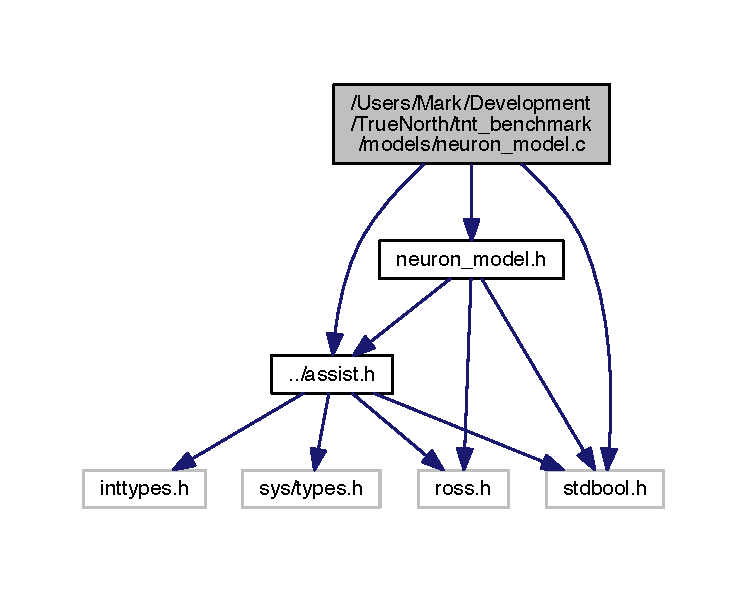
\includegraphics[width=350pt]{neuron__model_8c__incl}
\end{center}
\end{figure}
\subsection*{Functions}
\begin{DoxyCompactItemize}
\item 
void \hyperlink{neuron__model_8c_a6d548f86a3f6618241b7ffc5dd3ad374}{no\+Leak} (void $\ast$\hyperlink{structneuron_state}{neuron\+State}, tw\+\_\+stime end)
\item 
void \hyperlink{neuron__model_8c_a23e8b1105b7db3282e2b362edbb98f5a}{rev\+No\+Leak} (void $\ast$\hyperlink{structneuron_state}{neuron\+State}, tw\+\_\+stime now)
\item 
void \hyperlink{neuron__model_8c_a594e1a364caa704c44d60e8e815cc379}{linear\+Leak} (void $\ast$\hyperlink{structneuron_state}{neuron\+State}, tw\+\_\+stime end)
\item 
void \hyperlink{neuron__model_8c_a6d02e9cd19d8d6c7c3ce9db4ca63deaa}{synaptic\+Leak} (void $\ast$\hyperlink{structneuron_state}{neuron\+State}, tw\+\_\+stime end)
\item 
void \hyperlink{neuron__model_8c_a9166a79121534affadf20163b9af1ddb}{rev\+Linear\+Leak} (void $\ast$\hyperlink{structneuron_state}{neuron\+State}, tw\+\_\+stime now)
\item 
void \hyperlink{neuron__model_8c_a7f8eaa35f03747c795a2b727b364537b}{reset\+Zero} (void $\ast$\hyperlink{structneuron_state}{neuron\+State})
\begin{DoxyCompactList}\small\item\em Neuron Post-\/\+Fire reset functions\+: \end{DoxyCompactList}\item 
void \hyperlink{neuron__model_8c_a2e78d7d2b70bf7349c3854b3727dcc25}{reset\+Linear} (void $\ast$\hyperlink{structneuron_state}{neuron\+State})
\item 
void \hyperlink{neuron__model_8c_aabae9811b1573f5c38f4d32446c9c80a}{reverse\+Linear} (void $\ast$\hyperlink{structneuron_state}{neuron\+State})
\begin{DoxyCompactList}\small\item\em Neuron Post-\/\+Fire Reverse functions. \end{DoxyCompactList}\item 
void \hyperlink{neuron__model_8c_a286a9f9e22acec028acf23b62e13646b}{reverse\+Zero} (void $\ast$\hyperlink{structneuron_state}{neuron\+State})
\item 
bool \hyperlink{neuron__model_8c_acd4bc783d3c9dd73566599946b6aec9e}{neuron\+Receive\+Message} (\hyperlink{structneuron_state}{neuron\+State} $\ast$st, tw\+\_\+stime time, \hyperlink{struct_msg___data}{Msg\+\_\+\+Data} $\ast$m, tw\+\_\+lp $\ast$lp)
\begin{DoxyCompactList}\small\item\em neuron\+Receive\+Message -\/ a function that is the primary neuron message recipt handler. \end{DoxyCompactList}\item 
void \hyperlink{neuron__model_8c_ab1f4997e4bfe11e78faa6d37748aee67}{neuron\+Post\+Fire} (\hyperlink{structneuron_state}{neuron\+State} $\ast$st, tw\+\_\+stime time, \hyperlink{struct_msg___data}{Msg\+\_\+\+Data} $\ast$m)
\begin{DoxyCompactList}\small\item\em neuron\+Post\+Fire -\/ Function that cleans up the neuron state after firing. \end{DoxyCompactList}\item 
void \hyperlink{neuron__model_8c_ae071ef984b7e0dd4ec38fca91e0abe39}{neuron\+Fire} (\hyperlink{structneuron_state}{neuron\+State} $\ast$st, tw\+\_\+stime time, \hyperlink{struct_msg___data}{Msg\+\_\+\+Data} $\ast$m)
\begin{DoxyCompactList}\small\item\em neuron\+Fire Function called after firing status is determined to be true. \end{DoxyCompactList}\end{DoxyCompactItemize}


\subsection{Function Documentation}
\hypertarget{neuron__model_8c_a594e1a364caa704c44d60e8e815cc379}{}\index{neuron\+\_\+model.\+c@{neuron\+\_\+model.\+c}!linear\+Leak@{linear\+Leak}}
\index{linear\+Leak@{linear\+Leak}!neuron\+\_\+model.\+c@{neuron\+\_\+model.\+c}}
\subsubsection[{linear\+Leak}]{\setlength{\rightskip}{0pt plus 5cm}void linear\+Leak (
\begin{DoxyParamCaption}
\item[{void $\ast$}]{neuron\+State, }
\item[{tw\+\_\+stime}]{end}
\end{DoxyParamCaption}
)}\label{neuron__model_8c_a594e1a364caa704c44d60e8e815cc379}


Definition at line 15 of file neuron\+\_\+model.\+c.


\begin{DoxyCode}
15                                                 \{
16         \textcolor{comment}{//linear leak function. The rate is determined by the leak rate in the neuron.}
17     \textcolor{keyword}{struct }\hyperlink{struct_neuron_model}{NeuronModel} *s = (\textcolor{keyword}{struct }NueronModel *) \hyperlink{structneuron_state}{neuronState};
18     tw\_stime delta = end - s->lastLeakTime;
19     s->cVoltage -= s->leakRate * delta;
20     s->lastLeakTime = end;
21     
22 \}
\end{DoxyCode}
\hypertarget{neuron__model_8c_ae071ef984b7e0dd4ec38fca91e0abe39}{}\index{neuron\+\_\+model.\+c@{neuron\+\_\+model.\+c}!neuron\+Fire@{neuron\+Fire}}
\index{neuron\+Fire@{neuron\+Fire}!neuron\+\_\+model.\+c@{neuron\+\_\+model.\+c}}
\subsubsection[{neuron\+Fire}]{\setlength{\rightskip}{0pt plus 5cm}void neuron\+Fire (
\begin{DoxyParamCaption}
\item[{{\bf neuron\+State} $\ast$}]{st, }
\item[{tw\+\_\+stime}]{time, }
\item[{{\bf Msg\+\_\+\+Data} $\ast$}]{m}
\end{DoxyParamCaption}
)}\label{neuron__model_8c_ae071ef984b7e0dd4ec38fca91e0abe39}


neuron\+Fire Function called after firing status is determined to be true. 

Actual message is managed through \hyperlink{model__main_8c}{model\+\_\+main.\+c}. This function adjusts parameters for tracking neuron behaviors. 

Definition at line 143 of file neuron\+\_\+model.\+c.



References neuron\+State\+::fire\+Count.


\begin{DoxyCode}
143                                                              \{
144    st->\hyperlink{structneuron_state_a0658ad1f8b57a00589c6ea84f9a4ab13}{lastActiveTime}=time;
145    st->\hyperlink{structneuron_state_afc17c439bc3ffa469b045a7ceff7a25a}{fireCount} ++;
146 \}
\end{DoxyCode}
\hypertarget{neuron__model_8c_ab1f4997e4bfe11e78faa6d37748aee67}{}\index{neuron\+\_\+model.\+c@{neuron\+\_\+model.\+c}!neuron\+Post\+Fire@{neuron\+Post\+Fire}}
\index{neuron\+Post\+Fire@{neuron\+Post\+Fire}!neuron\+\_\+model.\+c@{neuron\+\_\+model.\+c}}
\subsubsection[{neuron\+Post\+Fire}]{\setlength{\rightskip}{0pt plus 5cm}void neuron\+Post\+Fire (
\begin{DoxyParamCaption}
\item[{{\bf neuron\+State} $\ast$}]{st, }
\item[{tw\+\_\+stime}]{time, }
\item[{{\bf Msg\+\_\+\+Data} $\ast$}]{m}
\end{DoxyParamCaption}
)}\label{neuron__model_8c_ab1f4997e4bfe11e78faa6d37748aee67}


neuron\+Post\+Fire -\/ Function that cleans up the neuron state after firing. 



Definition at line 132 of file neuron\+\_\+model.\+c.



References neuron\+State\+::do\+Reset.


\begin{DoxyCode}
132                                                                  \{
133    st->\hyperlink{structneuron_state_a0658ad1f8b57a00589c6ea84f9a4ab13}{lastActiveTime} = time;
134     
135    st->\hyperlink{structneuron_state_afcf9d931e4fda519c43b4efeab687463}{doReset}(st); \textcolor{comment}{// that may be a little fugly, but it does allow swapping of behaviors at
       runtime.}
136 
137 \}
\end{DoxyCode}
\hypertarget{neuron__model_8c_acd4bc783d3c9dd73566599946b6aec9e}{}\index{neuron\+\_\+model.\+c@{neuron\+\_\+model.\+c}!neuron\+Receive\+Message@{neuron\+Receive\+Message}}
\index{neuron\+Receive\+Message@{neuron\+Receive\+Message}!neuron\+\_\+model.\+c@{neuron\+\_\+model.\+c}}
\subsubsection[{neuron\+Receive\+Message}]{\setlength{\rightskip}{0pt plus 5cm}bool neuron\+Receive\+Message (
\begin{DoxyParamCaption}
\item[{{\bf neuron\+State} $\ast$}]{st, }
\item[{tw\+\_\+stime}]{time, }
\item[{{\bf Msg\+\_\+\+Data} $\ast$}]{m, }
\item[{tw\+\_\+lp $\ast$}]{lp}
\end{DoxyParamCaption}
)}\label{neuron__model_8c_acd4bc783d3c9dd73566599946b6aec9e}


neuron\+Receive\+Message -\/ a function that is the primary neuron message recipt handler. 

time The current timestamp (event timestamp)  st The state of the neuron  \hyperlink{struct_msg___data}{Msg\+\_\+\+Data} current message. Internal values will store this neuron\textquotesingle{}s previous state. \begin{DoxyReturn}{Returns}
bool A bool, true if the neuron has fired. 
\end{DoxyReturn}


Definition at line 80 of file neuron\+\_\+model.\+c.



References neuron\+State\+::c\+Voltage, neuron\+State\+::fire\+Mode, N\+F\+M, neuron\+State\+::per\+Synapse\+Det, neuron\+State\+::per\+Synapse\+Weight, Msg\+\_\+\+Data\+::prev\+Voltage, neuron\+State\+::pr\+Voltage, Msg\+\_\+\+Data\+::sender\+Local\+I\+D, and neuron\+State\+::threshold.


\begin{DoxyCode}
80                                                                                  \{
81    \textcolor{keywordtype}{bool} didFire = 0;
82    \textcolor{comment}{//prep the rotors ( reverse functions )}
83    \textcolor{comment}{//TODO: Move previous voltage to message.}
84    st->\hyperlink{structneuron_state_ac20c9ef5b5825eb38f91c1f1dacfb21d}{prVoltage} = st->\hyperlink{structneuron_state_a83c2516a958f81caedbaf4dd3c431d1b}{cVoltage};
85    m->\hyperlink{struct_msg___data_a20818fc301603eac9d3685ba53424699}{prevVoltage} = st->\hyperlink{structneuron_state_a83c2516a958f81caedbaf4dd3c431d1b}{cVoltage};
86    \textcolor{comment}{//prep complete. Now leaking based on time lapse:}
87 
88    st->\hyperlink{structneuron_state_ad0271f69fc01192f4f85b74d9bee06de}{leak}(st, time); \textcolor{comment}{//leak function call - do leak based on time passed since last communication.}
89 
90 
91    \textcolor{comment}{//apply weights & adjust our voltage:}
92 
93 
94    \hyperlink{assist_8h_a368ddcd71f7b61cb0f918f22d07ce999}{\_neVoltType} adjustedWeight;
95    \textcolor{keywordflow}{if} (st->\hyperlink{structneuron_state_a95688135a244a3ce3b35698a49d0da18}{perSynapseDet}[m->\hyperlink{struct_msg___data_af4e0329991e30bd3958b93c3bbb3038d}{senderLocalID}] == \textcolor{keyword}{true}) \{
96       adjustedWeight = st->\hyperlink{structneuron_state_ac21457aec3f29f9f28b58dd95e3d6fb2}{perSynapseWeight}[m->\hyperlink{struct_msg___data_af4e0329991e30bd3958b93c3bbb3038d}{senderLocalID}];
97       st->\hyperlink{structneuron_state_a83c2516a958f81caedbaf4dd3c431d1b}{cVoltage} += adjustedWeight;
98 
99            \textcolor{comment}{//next check for fire operations:}
100        \textcolor{keywordflow}{switch} (st->\hyperlink{structneuron_state_a55890f9e021064df30e9d18a9df98845}{fireMode}) \{
101            \textcolor{keywordflow}{case} \hyperlink{neuron__model_8h_a48885ea6be5b55a2e24de9f97552d4eea520c6b216334b8c2d914cf9fab8cd460}{NFM}:
102            \textcolor{keywordflow}{default}:
103                \textcolor{keywordflow}{if} (st->\hyperlink{structneuron_state_a83c2516a958f81caedbaf4dd3c431d1b}{cVoltage} >= st->\hyperlink{structneuron_state_ac3d7ce178528ec72b94fc0698be8213a}{threshold})\{
104                    didFire = \textcolor{keyword}{true};
105                    \hyperlink{neuron__model_8c_ae071ef984b7e0dd4ec38fca91e0abe39}{neuronFire}(st, time, m);
106                \}
107        \}
108    \}
109    \textcolor{keywordflow}{else} \{
110            \textcolor{comment}{//Stochastic fire mode:}
111            \textcolor{comment}{//from paper:}
112        \textcolor{comment}{/*For each neuron, each synaptic weight and leak has a configuration bit, bGij and cλ j
       respectively, where setting the bit to 0 selects deterministic mode, and 1 selects stochastic mode. For stochastic
       synaptic and leak integration, operation is as follows. }
113 \textcolor{comment}{        Every time a valid synaptic or leak event occurs, the neuron draws a uniformly distributed random
       number ρj. If the synaptic weight sGij or leak weight λj is greater than or equal to the drawn random number
       ρj, then the neuron integrates\{−1,+1\} otherwise, it does not integrate. */}
114            \textcolor{comment}{//This implementation uses}
115        \textcolor{comment}{//if(st->perSynapseWeight[m->senderLocalID] >=  tw\_rand\_unif(lp->rng))\{}
116                \textcolor{comment}{//fire here:}
117            didFire=\textcolor{keyword}{true};
118            \hyperlink{neuron__model_8c_ae071ef984b7e0dd4ec38fca91e0abe39}{neuronFire}(st, time, m);
119         \}
120 \textcolor{comment}{//   neuronFire(st, time, m); // call to fire function, however, not needed ATM.}
121 
122    \textcolor{keywordflow}{if}(didFire) \{
123       \hyperlink{neuron__model_8c_ab1f4997e4bfe11e78faa6d37748aee67}{neuronPostFire}(st, time, m);
124       
125    \}
126 
127    \textcolor{keywordflow}{return} didFire;
128 \}
\end{DoxyCode}
\hypertarget{neuron__model_8c_a6d548f86a3f6618241b7ffc5dd3ad374}{}\index{neuron\+\_\+model.\+c@{neuron\+\_\+model.\+c}!no\+Leak@{no\+Leak}}
\index{no\+Leak@{no\+Leak}!neuron\+\_\+model.\+c@{neuron\+\_\+model.\+c}}
\subsubsection[{no\+Leak}]{\setlength{\rightskip}{0pt plus 5cm}void no\+Leak (
\begin{DoxyParamCaption}
\item[{void $\ast$}]{neuron\+State, }
\item[{tw\+\_\+stime}]{end}
\end{DoxyParamCaption}
)}\label{neuron__model_8c_a6d548f86a3f6618241b7ffc5dd3ad374}


Definition at line 9 of file neuron\+\_\+model.\+c.


\begin{DoxyCode}
9                                              \{
10    \textcolor{comment}{//do nothing!!}
11 \}
\end{DoxyCode}
\hypertarget{neuron__model_8c_a2e78d7d2b70bf7349c3854b3727dcc25}{}\index{neuron\+\_\+model.\+c@{neuron\+\_\+model.\+c}!reset\+Linear@{reset\+Linear}}
\index{reset\+Linear@{reset\+Linear}!neuron\+\_\+model.\+c@{neuron\+\_\+model.\+c}}
\subsubsection[{reset\+Linear}]{\setlength{\rightskip}{0pt plus 5cm}void reset\+Linear (
\begin{DoxyParamCaption}
\item[{void $\ast$}]{neuron\+State}
\end{DoxyParamCaption}
)}\label{neuron__model_8c_a2e78d7d2b70bf7349c3854b3727dcc25}


Definition at line 50 of file neuron\+\_\+model.\+c.


\begin{DoxyCode}
50                                     \{
51     \textcolor{keyword}{struct }\hyperlink{struct_neuron_model}{NeuronModel} *s = (\textcolor{keyword}{struct }\hyperlink{struct_neuron_model}{NeuronModel} *) 
      \hyperlink{structneuron_state}{neuronState};
52         \textcolor{comment}{//reduce the value of the neuron based on the linear reduction function}
53         \textcolor{comment}{//in the paper}
54         \textcolor{comment}{//s->cVoltage = s->cVoltage - s->resetVoltParam;}
55 
56 \}
\end{DoxyCode}
\hypertarget{neuron__model_8c_a7f8eaa35f03747c795a2b727b364537b}{}\index{neuron\+\_\+model.\+c@{neuron\+\_\+model.\+c}!reset\+Zero@{reset\+Zero}}
\index{reset\+Zero@{reset\+Zero}!neuron\+\_\+model.\+c@{neuron\+\_\+model.\+c}}
\subsubsection[{reset\+Zero}]{\setlength{\rightskip}{0pt plus 5cm}void reset\+Zero (
\begin{DoxyParamCaption}
\item[{void $\ast$}]{neuron\+State}
\end{DoxyParamCaption}
)}\label{neuron__model_8c_a7f8eaa35f03747c795a2b727b364537b}


Neuron Post-\/\+Fire reset functions\+: 



Definition at line 39 of file neuron\+\_\+model.\+c.



References neuron\+State\+::c\+Voltage, and neuron\+State\+::pr\+Voltage.


\begin{DoxyCode}
39                                   \{
40    \textcolor{comment}{//State change happens here:}
41 
42    \textcolor{keyword}{struct }\hyperlink{struct_neuron_model}{NeuronModel} *s = (\textcolor{keyword}{struct }\hyperlink{struct_neuron_model}{NeuronModel} *) 
      \hyperlink{structneuron_state}{neuronState};
43    \textcolor{comment}{//ALL neuron functions called AFTER neuron msg rcvd and state saved.}
44    \textcolor{comment}{//s->prVoltage = s->cVoltage; // store current voltage in previous voltage holder.}
45     s->prVoltage = s->cVoltage;
46    s->cVoltage = 0; \textcolor{comment}{// set current voltage to 0.}
47 
48 \}
\end{DoxyCode}
\hypertarget{neuron__model_8c_aabae9811b1573f5c38f4d32446c9c80a}{}\index{neuron\+\_\+model.\+c@{neuron\+\_\+model.\+c}!reverse\+Linear@{reverse\+Linear}}
\index{reverse\+Linear@{reverse\+Linear}!neuron\+\_\+model.\+c@{neuron\+\_\+model.\+c}}
\subsubsection[{reverse\+Linear}]{\setlength{\rightskip}{0pt plus 5cm}void reverse\+Linear (
\begin{DoxyParamCaption}
\item[{void $\ast$}]{neuron\+State}
\end{DoxyParamCaption}
)}\label{neuron__model_8c_aabae9811b1573f5c38f4d32446c9c80a}


Neuron Post-\/\+Fire Reverse functions. 



Definition at line 61 of file neuron\+\_\+model.\+c.



References neuron\+State\+::c\+Voltage, and neuron\+State\+::reset\+Volt\+Param.


\begin{DoxyCode}
61                                       \{
62     \textcolor{keyword}{struct }\hyperlink{struct_neuron_model}{NeuronModel} *s = (\textcolor{keyword}{struct }\hyperlink{struct_neuron_model}{NeuronModel} *) 
      \hyperlink{structneuron_state}{neuronState};
63 
64     s->cVoltage = s->cVoltage + s->resetVoltParam;
65 \}
\end{DoxyCode}
\hypertarget{neuron__model_8c_a286a9f9e22acec028acf23b62e13646b}{}\index{neuron\+\_\+model.\+c@{neuron\+\_\+model.\+c}!reverse\+Zero@{reverse\+Zero}}
\index{reverse\+Zero@{reverse\+Zero}!neuron\+\_\+model.\+c@{neuron\+\_\+model.\+c}}
\subsubsection[{reverse\+Zero}]{\setlength{\rightskip}{0pt plus 5cm}void reverse\+Zero (
\begin{DoxyParamCaption}
\item[{void $\ast$}]{neuron\+State}
\end{DoxyParamCaption}
)}\label{neuron__model_8c_a286a9f9e22acec028acf23b62e13646b}


Definition at line 67 of file neuron\+\_\+model.\+c.



References neuron\+State\+::c\+Voltage, and neuron\+State\+::pr\+Voltage.


\begin{DoxyCode}
67                                     \{
68     \textcolor{keyword}{struct }\hyperlink{struct_neuron_model}{NeuronModel} *s = (\textcolor{keyword}{struct }\hyperlink{struct_neuron_model}{NeuronModel} *) 
      \hyperlink{structneuron_state}{neuronState};
69     s->cVoltage = s->prVoltage;
70 \}
\end{DoxyCode}
\hypertarget{neuron__model_8c_a9166a79121534affadf20163b9af1ddb}{}\index{neuron\+\_\+model.\+c@{neuron\+\_\+model.\+c}!rev\+Linear\+Leak@{rev\+Linear\+Leak}}
\index{rev\+Linear\+Leak@{rev\+Linear\+Leak}!neuron\+\_\+model.\+c@{neuron\+\_\+model.\+c}}
\subsubsection[{rev\+Linear\+Leak}]{\setlength{\rightskip}{0pt plus 5cm}void rev\+Linear\+Leak (
\begin{DoxyParamCaption}
\item[{void $\ast$}]{neuron\+State, }
\item[{tw\+\_\+stime}]{now}
\end{DoxyParamCaption}
)}\label{neuron__model_8c_a9166a79121534affadf20163b9af1ddb}


Definition at line 28 of file neuron\+\_\+model.\+c.


\begin{DoxyCode}
28                                                    \{
29 
30     \textcolor{keyword}{struct }\hyperlink{struct_neuron_model}{NeuronModel} *s =(\textcolor{keyword}{struct }\hyperlink{struct_neuron_model}{NeuronModel} *) 
      \hyperlink{structneuron_state}{neuronState};
31     tw\_stime delta = s->lastLeakTime - now;
32     s->cVoltage += s->leakRate * delta;
33     s->lastLeakTime = now;
34 \}
\end{DoxyCode}
\hypertarget{neuron__model_8c_a23e8b1105b7db3282e2b362edbb98f5a}{}\index{neuron\+\_\+model.\+c@{neuron\+\_\+model.\+c}!rev\+No\+Leak@{rev\+No\+Leak}}
\index{rev\+No\+Leak@{rev\+No\+Leak}!neuron\+\_\+model.\+c@{neuron\+\_\+model.\+c}}
\subsubsection[{rev\+No\+Leak}]{\setlength{\rightskip}{0pt plus 5cm}void rev\+No\+Leak (
\begin{DoxyParamCaption}
\item[{void $\ast$}]{neuron\+State, }
\item[{tw\+\_\+stime}]{now}
\end{DoxyParamCaption}
)}\label{neuron__model_8c_a23e8b1105b7db3282e2b362edbb98f5a}


Definition at line 12 of file neuron\+\_\+model.\+c.


\begin{DoxyCode}
12                                                \{
13         \textcolor{comment}{//do nothing!!}
14 \}
\end{DoxyCode}
\hypertarget{neuron__model_8c_a6d02e9cd19d8d6c7c3ce9db4ca63deaa}{}\index{neuron\+\_\+model.\+c@{neuron\+\_\+model.\+c}!synaptic\+Leak@{synaptic\+Leak}}
\index{synaptic\+Leak@{synaptic\+Leak}!neuron\+\_\+model.\+c@{neuron\+\_\+model.\+c}}
\subsubsection[{synaptic\+Leak}]{\setlength{\rightskip}{0pt plus 5cm}void synaptic\+Leak (
\begin{DoxyParamCaption}
\item[{void $\ast$}]{neuron\+State, }
\item[{tw\+\_\+stime}]{end}
\end{DoxyParamCaption}
)}\label{neuron__model_8c_a6d02e9cd19d8d6c7c3ce9db4ca63deaa}


Definition at line 23 of file neuron\+\_\+model.\+c.


\begin{DoxyCode}
23                                                    \{
24 \textcolor{comment}{//  struct NeuronModel *s = (struct NeuronModel *) neuronState;}
25 \textcolor{comment}{//  tw\_stime delta = end - s->lastLeakTime;}
26 \textcolor{comment}{//  s->cVoltage += }
27 \}
\end{DoxyCode}

\hypertarget{neuron__model_8h}{}\section{/\+Users/\+Mark/\+Development/\+True\+North/tnt\+\_\+benchmark/models/neuron\+\_\+model.h File Reference}
\label{neuron__model_8h}\index{/\+Users/\+Mark/\+Development/\+True\+North/tnt\+\_\+benchmark/models/neuron\+\_\+model.\+h@{/\+Users/\+Mark/\+Development/\+True\+North/tnt\+\_\+benchmark/models/neuron\+\_\+model.\+h}}
{\ttfamily \#include $<$stdbool.\+h$>$}\\*
{\ttfamily \#include \char`\"{}../assist.\+h\char`\"{}}\\*
{\ttfamily \#include \char`\"{}ross.\+h\char`\"{}}\\*
Include dependency graph for neuron\+\_\+model.\+h\+:\nopagebreak
\begin{figure}[H]
\begin{center}
\leavevmode
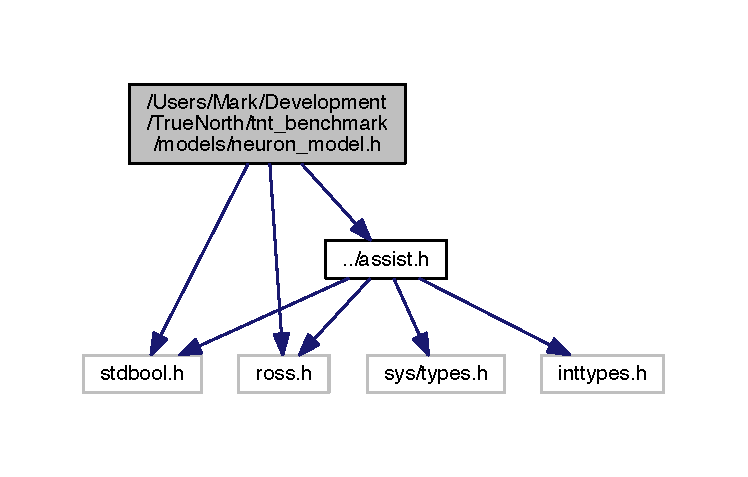
\includegraphics[width=350pt]{neuron__model_8h__incl}
\end{center}
\end{figure}
This graph shows which files directly or indirectly include this file\+:\nopagebreak
\begin{figure}[H]
\begin{center}
\leavevmode
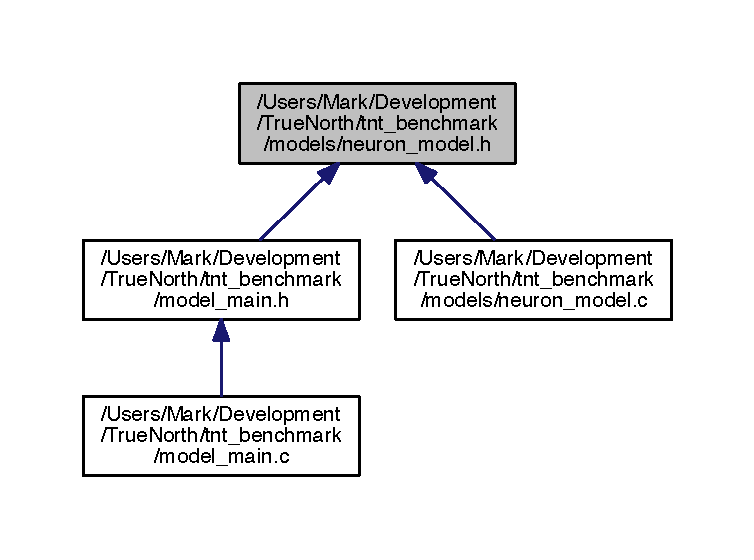
\includegraphics[width=350pt]{neuron__model_8h__dep__incl}
\end{center}
\end{figure}
\subsection*{Data Structures}
\begin{DoxyCompactItemize}
\item 
union \hyperlink{union_reset_rate}{Reset\+Rate}
\begin{DoxyCompactList}\small\item\em This is a support union for neuron reset rates. \end{DoxyCompactList}\item 
struct \hyperlink{structneuron_state}{neuron\+State}
\end{DoxyCompactItemize}
\subsection*{Typedefs}
\begin{DoxyCompactItemize}
\item 
typedef void($\ast$ \hyperlink{neuron__model_8h_a6eab2da39fb76cba9c4c54b5fb7625a6}{leak\+Fun\+Del}) (void $\ast$\hyperlink{structneuron_state}{neuron\+State}, tw\+\_\+stime end)
\item 
typedef void($\ast$ \hyperlink{neuron__model_8h_a960bf554f8c5333d901a15c49066f5b6}{reverse\+Leak\+Del}) (void $\ast$\hyperlink{structneuron_state}{neuron\+State}, tw\+\_\+stime now)
\item 
typedef void($\ast$ \hyperlink{neuron__model_8h_ae7e5990745cd949246894bfb633ca4a2}{reset\+Fun\+Del}) (void $\ast$\hyperlink{structneuron_state}{neuron\+State})
\begin{DoxyCompactList}\small\item\em Reset\+Fun\+Del -\/ This is a function that handles different reset rate calculations. \end{DoxyCompactList}\item 
typedef void($\ast$ \hyperlink{neuron__model_8h_aa939c0acc5b3367975f2f0cb7bc36d17}{reverse\+Reset\+Del}) (void $\ast$\hyperlink{structneuron_state}{neuron\+State})
\begin{DoxyCompactList}\small\item\em This is a function that reverses the reset command. \end{DoxyCompactList}\end{DoxyCompactItemize}
\subsection*{Enumerations}
\begin{DoxyCompactItemize}
\item 
enum \hyperlink{neuron__model_8h_a48885ea6be5b55a2e24de9f97552d4ee}{neuron\+Fire\+Mode} \{ \hyperlink{neuron__model_8h_a48885ea6be5b55a2e24de9f97552d4eea520c6b216334b8c2d914cf9fab8cd460}{N\+F\+M} = 0
 \}
\begin{DoxyCompactList}\small\item\em Simplified neuron model for benchmarking. \end{DoxyCompactList}\end{DoxyCompactItemize}
\subsection*{Functions}
\begin{DoxyCompactItemize}
\item 
void \hyperlink{neuron__model_8h_a6d548f86a3f6618241b7ffc5dd3ad374}{no\+Leak} (void $\ast$\hyperlink{structneuron_state}{neuron\+State}, tw\+\_\+stime end)
\item 
void \hyperlink{neuron__model_8h_a23e8b1105b7db3282e2b362edbb98f5a}{rev\+No\+Leak} (void $\ast$\hyperlink{structneuron_state}{neuron\+State}, tw\+\_\+stime now)
\item 
void \hyperlink{neuron__model_8h_a7f8eaa35f03747c795a2b727b364537b}{reset\+Zero} (void $\ast$\hyperlink{structneuron_state}{neuron\+State})
\begin{DoxyCompactList}\small\item\em Neuron Post-\/\+Fire reset functions\+: \end{DoxyCompactList}\item 
void \hyperlink{neuron__model_8h_a2e78d7d2b70bf7349c3854b3727dcc25}{reset\+Linear} (void $\ast$\hyperlink{structneuron_state}{neuron\+State})
\item 
void \hyperlink{neuron__model_8h_aabae9811b1573f5c38f4d32446c9c80a}{reverse\+Linear} (void $\ast$\hyperlink{structneuron_state}{neuron\+State})
\begin{DoxyCompactList}\small\item\em Neuron Post-\/\+Fire Reverse functions. \end{DoxyCompactList}\item 
void \hyperlink{neuron__model_8h_a286a9f9e22acec028acf23b62e13646b}{reverse\+Zero} (void $\ast$\hyperlink{structneuron_state}{neuron\+State})
\item 
bool \hyperlink{neuron__model_8h_acd4bc783d3c9dd73566599946b6aec9e}{neuron\+Receive\+Message} (\hyperlink{structneuron_state}{neuron\+State} $\ast$st, tw\+\_\+stime time, \hyperlink{struct_msg___data}{Msg\+\_\+\+Data} $\ast$m, tw\+\_\+lp $\ast$lp)
\begin{DoxyCompactList}\small\item\em neuron\+Receive\+Message -\/ a function that is the primary neuron message recipt handler. \end{DoxyCompactList}\item 
void \hyperlink{neuron__model_8h_ae071ef984b7e0dd4ec38fca91e0abe39}{neuron\+Fire} (\hyperlink{structneuron_state}{neuron\+State} $\ast$st, tw\+\_\+stime time, \hyperlink{struct_msg___data}{Msg\+\_\+\+Data} $\ast$m)
\begin{DoxyCompactList}\small\item\em neuron\+Fire Function called after firing status is determined to be true. \end{DoxyCompactList}\item 
void \hyperlink{neuron__model_8h_ab1f4997e4bfe11e78faa6d37748aee67}{neuron\+Post\+Fire} (\hyperlink{structneuron_state}{neuron\+State} $\ast$st, tw\+\_\+stime time, \hyperlink{struct_msg___data}{Msg\+\_\+\+Data} $\ast$m)
\begin{DoxyCompactList}\small\item\em neuron\+Post\+Fire -\/ Function that cleans up the neuron state after firing. \end{DoxyCompactList}\end{DoxyCompactItemize}
\subsection*{Variables}
\begin{DoxyCompactItemize}
\item 
union \hyperlink{union_reset_rate}{Reset\+Rate} \hyperlink{neuron__model_8h_ad0ba8fdd39dc976fd20fe0a684041c16}{reset\+Rate}
\end{DoxyCompactItemize}


\subsection{Typedef Documentation}
\hypertarget{neuron__model_8h_a6eab2da39fb76cba9c4c54b5fb7625a6}{}\index{neuron\+\_\+model.\+h@{neuron\+\_\+model.\+h}!leak\+Fun\+Del@{leak\+Fun\+Del}}
\index{leak\+Fun\+Del@{leak\+Fun\+Del}!neuron\+\_\+model.\+h@{neuron\+\_\+model.\+h}}
\subsubsection[{leak\+Fun\+Del}]{\setlength{\rightskip}{0pt plus 5cm}typedef void($\ast$ {\bf leak\+Fun\+Del}) (void $\ast${\bf neuron\+State}, tw\+\_\+stime end)}\label{neuron__model_8h_a6eab2da39fb76cba9c4c54b5fb7625a6}


Definition at line 33 of file neuron\+\_\+model.\+h.

\hypertarget{neuron__model_8h_ae7e5990745cd949246894bfb633ca4a2}{}\index{neuron\+\_\+model.\+h@{neuron\+\_\+model.\+h}!reset\+Fun\+Del@{reset\+Fun\+Del}}
\index{reset\+Fun\+Del@{reset\+Fun\+Del}!neuron\+\_\+model.\+h@{neuron\+\_\+model.\+h}}
\subsubsection[{reset\+Fun\+Del}]{\setlength{\rightskip}{0pt plus 5cm}typedef void($\ast$ reset\+Fun\+Del) (void $\ast${\bf neuron\+State})}\label{neuron__model_8h_ae7e5990745cd949246894bfb633ca4a2}


Reset\+Fun\+Del -\/ This is a function that handles different reset rate calculations. 

It takes the state of the neuron, and applies various reset functions to the neuron\textquotesingle{}s voltage. Some reset functions described by true north include a zeroing function (standard integrate and fire), a linear drop function, and a non-\/reduction function. Also functions for leaks below. 

Definition at line 55 of file neuron\+\_\+model.\+h.

\hypertarget{neuron__model_8h_a960bf554f8c5333d901a15c49066f5b6}{}\index{neuron\+\_\+model.\+h@{neuron\+\_\+model.\+h}!reverse\+Leak\+Del@{reverse\+Leak\+Del}}
\index{reverse\+Leak\+Del@{reverse\+Leak\+Del}!neuron\+\_\+model.\+h@{neuron\+\_\+model.\+h}}
\subsubsection[{reverse\+Leak\+Del}]{\setlength{\rightskip}{0pt plus 5cm}typedef void($\ast$ {\bf reverse\+Leak\+Del}) (void $\ast${\bf neuron\+State}, tw\+\_\+stime now)}\label{neuron__model_8h_a960bf554f8c5333d901a15c49066f5b6}


Definition at line 40 of file neuron\+\_\+model.\+h.

\hypertarget{neuron__model_8h_aa939c0acc5b3367975f2f0cb7bc36d17}{}\index{neuron\+\_\+model.\+h@{neuron\+\_\+model.\+h}!reverse\+Reset\+Del@{reverse\+Reset\+Del}}
\index{reverse\+Reset\+Del@{reverse\+Reset\+Del}!neuron\+\_\+model.\+h@{neuron\+\_\+model.\+h}}
\subsubsection[{reverse\+Reset\+Del}]{\setlength{\rightskip}{0pt plus 5cm}reverse\+Reset\+Del}\label{neuron__model_8h_aa939c0acc5b3367975f2f0cb7bc36d17}


This is a function that reverses the reset command. 

Run first, since the reset function is run last. 

Definition at line 66 of file neuron\+\_\+model.\+h.



\subsection{Enumeration Type Documentation}
\hypertarget{neuron__model_8h_a48885ea6be5b55a2e24de9f97552d4ee}{}\index{neuron\+\_\+model.\+h@{neuron\+\_\+model.\+h}!neuron\+Fire\+Mode@{neuron\+Fire\+Mode}}
\index{neuron\+Fire\+Mode@{neuron\+Fire\+Mode}!neuron\+\_\+model.\+h@{neuron\+\_\+model.\+h}}
\subsubsection[{neuron\+Fire\+Mode}]{\setlength{\rightskip}{0pt plus 5cm}enum {\bf neuron\+Fire\+Mode}}\label{neuron__model_8h_a48885ea6be5b55a2e24de9f97552d4ee}


Simplified neuron model for benchmarking. 

typedef Neuron\+Fire\+Mode Just in case there are multiple fire modes, this enum exists to differentiate them. \begin{Desc}
\item[Enumerator]\par
\begin{description}
\index{N\+F\+M@{N\+F\+M}!neuron\+\_\+model.\+h@{neuron\+\_\+model.\+h}}\index{neuron\+\_\+model.\+h@{neuron\+\_\+model.\+h}!N\+F\+M@{N\+F\+M}}\item[{\em 
\hypertarget{neuron__model_8h_a48885ea6be5b55a2e24de9f97552d4eea520c6b216334b8c2d914cf9fab8cd460}{}N\+F\+M\label{neuron__model_8h_a48885ea6be5b55a2e24de9f97552d4eea520c6b216334b8c2d914cf9fab8cd460}
}]\end{description}
\end{Desc}


Definition at line 23 of file neuron\+\_\+model.\+h.


\begin{DoxyCode}
23                            \{
24     \hyperlink{neuron__model_8h_a48885ea6be5b55a2e24de9f97552d4eea520c6b216334b8c2d914cf9fab8cd460}{NFM} = 0 \textcolor{comment}{// normal fire mode (if voltage > threshold, fire);}
25 \} \hyperlink{neuron__model_8h_a48885ea6be5b55a2e24de9f97552d4ee}{neuronFireMode};
\end{DoxyCode}


\subsection{Function Documentation}
\hypertarget{neuron__model_8h_ae071ef984b7e0dd4ec38fca91e0abe39}{}\index{neuron\+\_\+model.\+h@{neuron\+\_\+model.\+h}!neuron\+Fire@{neuron\+Fire}}
\index{neuron\+Fire@{neuron\+Fire}!neuron\+\_\+model.\+h@{neuron\+\_\+model.\+h}}
\subsubsection[{neuron\+Fire}]{\setlength{\rightskip}{0pt plus 5cm}void neuron\+Fire (
\begin{DoxyParamCaption}
\item[{{\bf neuron\+State} $\ast$}]{st, }
\item[{tw\+\_\+stime}]{time, }
\item[{{\bf Msg\+\_\+\+Data} $\ast$}]{m}
\end{DoxyParamCaption}
)}\label{neuron__model_8h_ae071ef984b7e0dd4ec38fca91e0abe39}


neuron\+Fire Function called after firing status is determined to be true. 

Actual message is managed through \hyperlink{model__main_8c}{model\+\_\+main.\+c}. This function adjusts parameters for tracking neuron behaviors. 

Definition at line 143 of file neuron\+\_\+model.\+c.



References neuron\+State\+::fire\+Count.


\begin{DoxyCode}
143                                                              \{
144    st->\hyperlink{structneuron_state_a0658ad1f8b57a00589c6ea84f9a4ab13}{lastActiveTime}=time;
145    st->\hyperlink{structneuron_state_afc17c439bc3ffa469b045a7ceff7a25a}{fireCount} ++;
146 \}
\end{DoxyCode}
\hypertarget{neuron__model_8h_ab1f4997e4bfe11e78faa6d37748aee67}{}\index{neuron\+\_\+model.\+h@{neuron\+\_\+model.\+h}!neuron\+Post\+Fire@{neuron\+Post\+Fire}}
\index{neuron\+Post\+Fire@{neuron\+Post\+Fire}!neuron\+\_\+model.\+h@{neuron\+\_\+model.\+h}}
\subsubsection[{neuron\+Post\+Fire}]{\setlength{\rightskip}{0pt plus 5cm}void neuron\+Post\+Fire (
\begin{DoxyParamCaption}
\item[{{\bf neuron\+State} $\ast$}]{st, }
\item[{tw\+\_\+stime}]{time, }
\item[{{\bf Msg\+\_\+\+Data} $\ast$}]{m}
\end{DoxyParamCaption}
)}\label{neuron__model_8h_ab1f4997e4bfe11e78faa6d37748aee67}


neuron\+Post\+Fire -\/ Function that cleans up the neuron state after firing. 



Definition at line 132 of file neuron\+\_\+model.\+c.



References neuron\+State\+::do\+Reset.


\begin{DoxyCode}
132                                                                  \{
133    st->\hyperlink{structneuron_state_a0658ad1f8b57a00589c6ea84f9a4ab13}{lastActiveTime} = time;
134     
135    st->\hyperlink{structneuron_state_afcf9d931e4fda519c43b4efeab687463}{doReset}(st); \textcolor{comment}{// that may be a little fugly, but it does allow swapping of behaviors at
       runtime.}
136 
137 \}
\end{DoxyCode}
\hypertarget{neuron__model_8h_acd4bc783d3c9dd73566599946b6aec9e}{}\index{neuron\+\_\+model.\+h@{neuron\+\_\+model.\+h}!neuron\+Receive\+Message@{neuron\+Receive\+Message}}
\index{neuron\+Receive\+Message@{neuron\+Receive\+Message}!neuron\+\_\+model.\+h@{neuron\+\_\+model.\+h}}
\subsubsection[{neuron\+Receive\+Message}]{\setlength{\rightskip}{0pt plus 5cm}bool neuron\+Receive\+Message (
\begin{DoxyParamCaption}
\item[{{\bf neuron\+State} $\ast$}]{st, }
\item[{tw\+\_\+stime}]{time, }
\item[{{\bf Msg\+\_\+\+Data} $\ast$}]{m, }
\item[{tw\+\_\+lp $\ast$}]{lp}
\end{DoxyParamCaption}
)}\label{neuron__model_8h_acd4bc783d3c9dd73566599946b6aec9e}


neuron\+Receive\+Message -\/ a function that is the primary neuron message recipt handler. 

time The current timestamp (event timestamp)  st The state of the neuron  \hyperlink{struct_msg___data}{Msg\+\_\+\+Data} current message. Internal values will store this neuron\textquotesingle{}s previous state. \begin{DoxyReturn}{Returns}
bool A bool, true if the neuron has fired. 
\end{DoxyReturn}


Definition at line 80 of file neuron\+\_\+model.\+c.



References neuron\+State\+::c\+Voltage, neuron\+State\+::fire\+Mode, N\+F\+M, neuron\+State\+::per\+Synapse\+Det, neuron\+State\+::per\+Synapse\+Weight, Msg\+\_\+\+Data\+::prev\+Voltage, neuron\+State\+::pr\+Voltage, Msg\+\_\+\+Data\+::sender\+Local\+I\+D, and neuron\+State\+::threshold.


\begin{DoxyCode}
80                                                                                  \{
81    \textcolor{keywordtype}{bool} didFire = 0;
82    \textcolor{comment}{//prep the rotors ( reverse functions )}
83    \textcolor{comment}{//TODO: Move previous voltage to message.}
84    st->\hyperlink{structneuron_state_ac20c9ef5b5825eb38f91c1f1dacfb21d}{prVoltage} = st->\hyperlink{structneuron_state_a83c2516a958f81caedbaf4dd3c431d1b}{cVoltage};
85    m->\hyperlink{struct_msg___data_a20818fc301603eac9d3685ba53424699}{prevVoltage} = st->\hyperlink{structneuron_state_a83c2516a958f81caedbaf4dd3c431d1b}{cVoltage};
86    \textcolor{comment}{//prep complete. Now leaking based on time lapse:}
87 
88    st->\hyperlink{structneuron_state_ad0271f69fc01192f4f85b74d9bee06de}{leak}(st, time); \textcolor{comment}{//leak function call - do leak based on time passed since last communication.}
89 
90 
91    \textcolor{comment}{//apply weights & adjust our voltage:}
92 
93 
94    \hyperlink{assist_8h_a368ddcd71f7b61cb0f918f22d07ce999}{\_neVoltType} adjustedWeight;
95    \textcolor{keywordflow}{if} (st->\hyperlink{structneuron_state_a95688135a244a3ce3b35698a49d0da18}{perSynapseDet}[m->\hyperlink{struct_msg___data_af4e0329991e30bd3958b93c3bbb3038d}{senderLocalID}] == \textcolor{keyword}{true}) \{
96       adjustedWeight = st->\hyperlink{structneuron_state_ac21457aec3f29f9f28b58dd95e3d6fb2}{perSynapseWeight}[m->\hyperlink{struct_msg___data_af4e0329991e30bd3958b93c3bbb3038d}{senderLocalID}];
97       st->\hyperlink{structneuron_state_a83c2516a958f81caedbaf4dd3c431d1b}{cVoltage} += adjustedWeight;
98 
99            \textcolor{comment}{//next check for fire operations:}
100        \textcolor{keywordflow}{switch} (st->\hyperlink{structneuron_state_a55890f9e021064df30e9d18a9df98845}{fireMode}) \{
101            \textcolor{keywordflow}{case} \hyperlink{neuron__model_8h_a48885ea6be5b55a2e24de9f97552d4eea520c6b216334b8c2d914cf9fab8cd460}{NFM}:
102            \textcolor{keywordflow}{default}:
103                \textcolor{keywordflow}{if} (st->\hyperlink{structneuron_state_a83c2516a958f81caedbaf4dd3c431d1b}{cVoltage} >= st->\hyperlink{structneuron_state_ac3d7ce178528ec72b94fc0698be8213a}{threshold})\{
104                    didFire = \textcolor{keyword}{true};
105                    \hyperlink{neuron__model_8c_ae071ef984b7e0dd4ec38fca91e0abe39}{neuronFire}(st, time, m);
106                \}
107        \}
108    \}
109    \textcolor{keywordflow}{else} \{
110            \textcolor{comment}{//Stochastic fire mode:}
111            \textcolor{comment}{//from paper:}
112        \textcolor{comment}{/*For each neuron, each synaptic weight and leak has a configuration bit, bGij and cλ j
       respectively, where setting the bit to 0 selects deterministic mode, and 1 selects stochastic mode. For stochastic
       synaptic and leak integration, operation is as follows. }
113 \textcolor{comment}{        Every time a valid synaptic or leak event occurs, the neuron draws a uniformly distributed random
       number ρj. If the synaptic weight sGij or leak weight λj is greater than or equal to the drawn random number
       ρj, then the neuron integrates\{−1,+1\} otherwise, it does not integrate. */}
114            \textcolor{comment}{//This implementation uses}
115        \textcolor{comment}{//if(st->perSynapseWeight[m->senderLocalID] >=  tw\_rand\_unif(lp->rng))\{}
116                \textcolor{comment}{//fire here:}
117            didFire=\textcolor{keyword}{true};
118            \hyperlink{neuron__model_8c_ae071ef984b7e0dd4ec38fca91e0abe39}{neuronFire}(st, time, m);
119         \}
120 \textcolor{comment}{//   neuronFire(st, time, m); // call to fire function, however, not needed ATM.}
121 
122    \textcolor{keywordflow}{if}(didFire) \{
123       \hyperlink{neuron__model_8c_ab1f4997e4bfe11e78faa6d37748aee67}{neuronPostFire}(st, time, m);
124       
125    \}
126 
127    \textcolor{keywordflow}{return} didFire;
128 \}
\end{DoxyCode}
\hypertarget{neuron__model_8h_a6d548f86a3f6618241b7ffc5dd3ad374}{}\index{neuron\+\_\+model.\+h@{neuron\+\_\+model.\+h}!no\+Leak@{no\+Leak}}
\index{no\+Leak@{no\+Leak}!neuron\+\_\+model.\+h@{neuron\+\_\+model.\+h}}
\subsubsection[{no\+Leak}]{\setlength{\rightskip}{0pt plus 5cm}void no\+Leak (
\begin{DoxyParamCaption}
\item[{void $\ast$}]{neuron\+State, }
\item[{tw\+\_\+stime}]{end}
\end{DoxyParamCaption}
)}\label{neuron__model_8h_a6d548f86a3f6618241b7ffc5dd3ad374}


Definition at line 9 of file neuron\+\_\+model.\+c.


\begin{DoxyCode}
9                                              \{
10    \textcolor{comment}{//do nothing!!}
11 \}
\end{DoxyCode}
\hypertarget{neuron__model_8h_a2e78d7d2b70bf7349c3854b3727dcc25}{}\index{neuron\+\_\+model.\+h@{neuron\+\_\+model.\+h}!reset\+Linear@{reset\+Linear}}
\index{reset\+Linear@{reset\+Linear}!neuron\+\_\+model.\+h@{neuron\+\_\+model.\+h}}
\subsubsection[{reset\+Linear}]{\setlength{\rightskip}{0pt plus 5cm}void reset\+Linear (
\begin{DoxyParamCaption}
\item[{void $\ast$}]{neuron\+State}
\end{DoxyParamCaption}
)}\label{neuron__model_8h_a2e78d7d2b70bf7349c3854b3727dcc25}


Definition at line 50 of file neuron\+\_\+model.\+c.


\begin{DoxyCode}
50                                     \{
51     \textcolor{keyword}{struct }\hyperlink{struct_neuron_model}{NeuronModel} *s = (\textcolor{keyword}{struct }\hyperlink{struct_neuron_model}{NeuronModel} *) 
      \hyperlink{structneuron_state}{neuronState};
52         \textcolor{comment}{//reduce the value of the neuron based on the linear reduction function}
53         \textcolor{comment}{//in the paper}
54         \textcolor{comment}{//s->cVoltage = s->cVoltage - s->resetVoltParam;}
55 
56 \}
\end{DoxyCode}
\hypertarget{neuron__model_8h_a7f8eaa35f03747c795a2b727b364537b}{}\index{neuron\+\_\+model.\+h@{neuron\+\_\+model.\+h}!reset\+Zero@{reset\+Zero}}
\index{reset\+Zero@{reset\+Zero}!neuron\+\_\+model.\+h@{neuron\+\_\+model.\+h}}
\subsubsection[{reset\+Zero}]{\setlength{\rightskip}{0pt plus 5cm}void reset\+Zero (
\begin{DoxyParamCaption}
\item[{void $\ast$}]{neuron\+State}
\end{DoxyParamCaption}
)}\label{neuron__model_8h_a7f8eaa35f03747c795a2b727b364537b}


Neuron Post-\/\+Fire reset functions\+: 



Definition at line 39 of file neuron\+\_\+model.\+c.



References neuron\+State\+::c\+Voltage, and neuron\+State\+::pr\+Voltage.


\begin{DoxyCode}
39                                   \{
40    \textcolor{comment}{//State change happens here:}
41 
42    \textcolor{keyword}{struct }\hyperlink{struct_neuron_model}{NeuronModel} *s = (\textcolor{keyword}{struct }\hyperlink{struct_neuron_model}{NeuronModel} *) 
      \hyperlink{structneuron_state}{neuronState};
43    \textcolor{comment}{//ALL neuron functions called AFTER neuron msg rcvd and state saved.}
44    \textcolor{comment}{//s->prVoltage = s->cVoltage; // store current voltage in previous voltage holder.}
45     s->prVoltage = s->cVoltage;
46    s->cVoltage = 0; \textcolor{comment}{// set current voltage to 0.}
47 
48 \}
\end{DoxyCode}
\hypertarget{neuron__model_8h_aabae9811b1573f5c38f4d32446c9c80a}{}\index{neuron\+\_\+model.\+h@{neuron\+\_\+model.\+h}!reverse\+Linear@{reverse\+Linear}}
\index{reverse\+Linear@{reverse\+Linear}!neuron\+\_\+model.\+h@{neuron\+\_\+model.\+h}}
\subsubsection[{reverse\+Linear}]{\setlength{\rightskip}{0pt plus 5cm}void reverse\+Linear (
\begin{DoxyParamCaption}
\item[{void $\ast$}]{neuron\+State}
\end{DoxyParamCaption}
)}\label{neuron__model_8h_aabae9811b1573f5c38f4d32446c9c80a}


Neuron Post-\/\+Fire Reverse functions. 



Definition at line 61 of file neuron\+\_\+model.\+c.



References neuron\+State\+::c\+Voltage, and neuron\+State\+::reset\+Volt\+Param.


\begin{DoxyCode}
61                                       \{
62     \textcolor{keyword}{struct }\hyperlink{struct_neuron_model}{NeuronModel} *s = (\textcolor{keyword}{struct }\hyperlink{struct_neuron_model}{NeuronModel} *) 
      \hyperlink{structneuron_state}{neuronState};
63 
64     s->cVoltage = s->cVoltage + s->resetVoltParam;
65 \}
\end{DoxyCode}
\hypertarget{neuron__model_8h_a286a9f9e22acec028acf23b62e13646b}{}\index{neuron\+\_\+model.\+h@{neuron\+\_\+model.\+h}!reverse\+Zero@{reverse\+Zero}}
\index{reverse\+Zero@{reverse\+Zero}!neuron\+\_\+model.\+h@{neuron\+\_\+model.\+h}}
\subsubsection[{reverse\+Zero}]{\setlength{\rightskip}{0pt plus 5cm}void reverse\+Zero (
\begin{DoxyParamCaption}
\item[{void $\ast$}]{neuron\+State}
\end{DoxyParamCaption}
)}\label{neuron__model_8h_a286a9f9e22acec028acf23b62e13646b}


Definition at line 67 of file neuron\+\_\+model.\+c.



References neuron\+State\+::c\+Voltage, and neuron\+State\+::pr\+Voltage.


\begin{DoxyCode}
67                                     \{
68     \textcolor{keyword}{struct }\hyperlink{struct_neuron_model}{NeuronModel} *s = (\textcolor{keyword}{struct }\hyperlink{struct_neuron_model}{NeuronModel} *) 
      \hyperlink{structneuron_state}{neuronState};
69     s->cVoltage = s->prVoltage;
70 \}
\end{DoxyCode}
\hypertarget{neuron__model_8h_a23e8b1105b7db3282e2b362edbb98f5a}{}\index{neuron\+\_\+model.\+h@{neuron\+\_\+model.\+h}!rev\+No\+Leak@{rev\+No\+Leak}}
\index{rev\+No\+Leak@{rev\+No\+Leak}!neuron\+\_\+model.\+h@{neuron\+\_\+model.\+h}}
\subsubsection[{rev\+No\+Leak}]{\setlength{\rightskip}{0pt plus 5cm}void rev\+No\+Leak (
\begin{DoxyParamCaption}
\item[{void $\ast$}]{neuron\+State, }
\item[{tw\+\_\+stime}]{now}
\end{DoxyParamCaption}
)}\label{neuron__model_8h_a23e8b1105b7db3282e2b362edbb98f5a}


Definition at line 12 of file neuron\+\_\+model.\+c.


\begin{DoxyCode}
12                                                \{
13         \textcolor{comment}{//do nothing!!}
14 \}
\end{DoxyCode}


\subsection{Variable Documentation}
\hypertarget{neuron__model_8h_ad0ba8fdd39dc976fd20fe0a684041c16}{}\index{neuron\+\_\+model.\+h@{neuron\+\_\+model.\+h}!reset\+Rate@{reset\+Rate}}
\index{reset\+Rate@{reset\+Rate}!neuron\+\_\+model.\+h@{neuron\+\_\+model.\+h}}
\subsubsection[{reset\+Rate}]{\setlength{\rightskip}{0pt plus 5cm}union {\bf Reset\+Rate} reset\+Rate}\label{neuron__model_8h_ad0ba8fdd39dc976fd20fe0a684041c16}

\hypertarget{synapse_8h}{}\section{/\+Users/\+Mark/\+Development/\+True\+North/tnt\+\_\+benchmark/models/synapse.h File Reference}
\label{synapse_8h}\index{/\+Users/\+Mark/\+Development/\+True\+North/tnt\+\_\+benchmark/models/synapse.\+h@{/\+Users/\+Mark/\+Development/\+True\+North/tnt\+\_\+benchmark/models/synapse.\+h}}
{\ttfamily \#include $<$stdio.\+h$>$}\\*
{\ttfamily \#include \char`\"{}../assist.\+h\char`\"{}}\\*
{\ttfamily \#include \char`\"{}../input\+\_\+simulator.\+h\char`\"{}}\\*
Include dependency graph for synapse.\+h\+:
\nopagebreak
\begin{figure}[H]
\begin{center}
\leavevmode
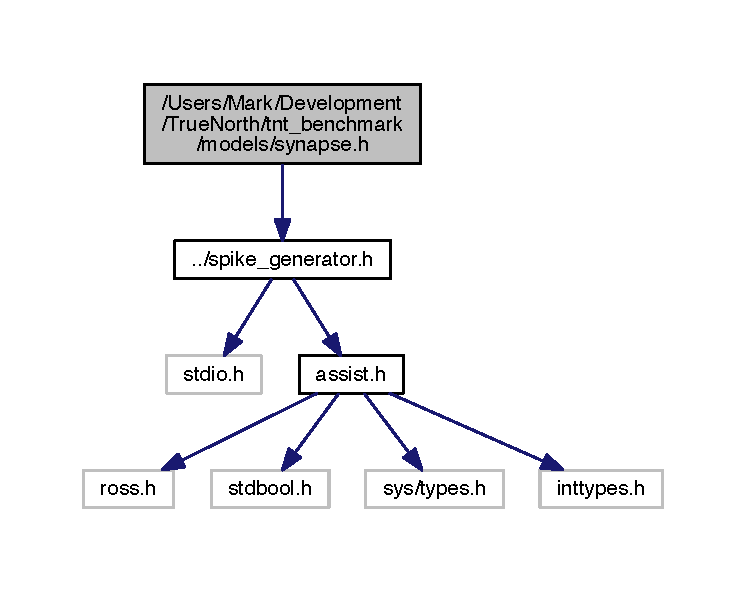
\includegraphics[width=344pt]{synapse_8h__incl}
\end{center}
\end{figure}
This graph shows which files directly or indirectly include this file\+:
\nopagebreak
\begin{figure}[H]
\begin{center}
\leavevmode
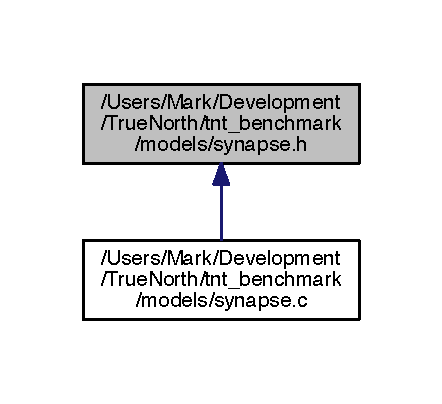
\includegraphics[width=212pt]{synapse_8h__dep__incl}
\end{center}
\end{figure}
\subsection*{Data Structures}
\begin{DoxyCompactItemize}
\item 
struct \hyperlink{structsynapse_state}{synapse\+State}
\begin{DoxyCompactList}\small\item\em Synapse state structure. \end{DoxyCompactList}\end{DoxyCompactItemize}

\hypertarget{spike__generator_8c}{}\section{/\+Users/\+Mark/\+Development/\+True\+North/tnt\+\_\+benchmark/spike\+\_\+generator.c File Reference}
\label{spike__generator_8c}\index{/\+Users/\+Mark/\+Development/\+True\+North/tnt\+\_\+benchmark/spike\+\_\+generator.\+c@{/\+Users/\+Mark/\+Development/\+True\+North/tnt\+\_\+benchmark/spike\+\_\+generator.\+c}}
{\ttfamily \#include \char`\"{}spike\+\_\+generator.\+h\char`\"{}}\\*
Include dependency graph for spike\+\_\+generator.\+c\+:\nopagebreak
\begin{figure}[H]
\begin{center}
\leavevmode
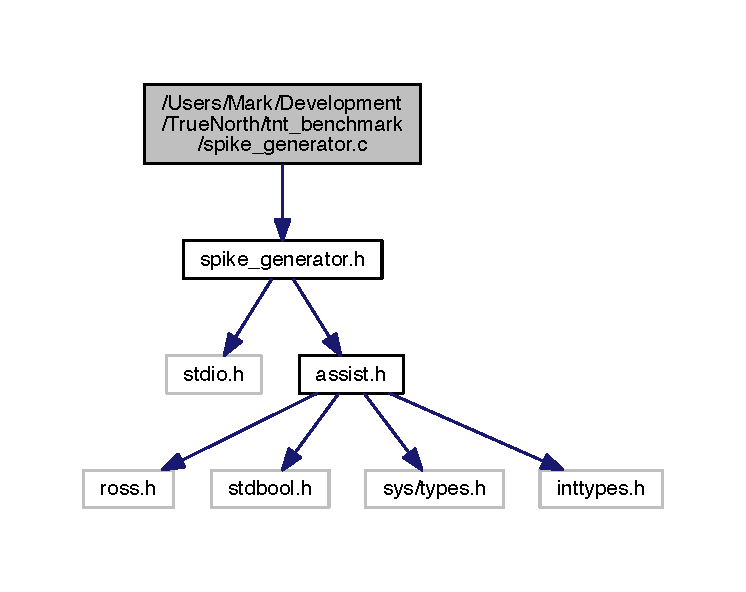
\includegraphics[width=350pt]{spike__generator_8c__incl}
\end{center}
\end{figure}
\subsection*{Functions}
\begin{DoxyCompactItemize}
\item 
bool \hyperlink{spike__generator_8c_a7ffa6df128d9c249ace6677ae62d1723}{uniform\+Gen} (void $\ast$spike\+Gen, tw\+\_\+lp $\ast$lp)
\end{DoxyCompactItemize}


\subsection{Function Documentation}
\hypertarget{spike__generator_8c_a7ffa6df128d9c249ace6677ae62d1723}{}\index{spike\+\_\+generator.\+c@{spike\+\_\+generator.\+c}!uniform\+Gen@{uniform\+Gen}}
\index{uniform\+Gen@{uniform\+Gen}!spike\+\_\+generator.\+c@{spike\+\_\+generator.\+c}}
\subsubsection[{uniform\+Gen}]{\setlength{\rightskip}{0pt plus 5cm}bool uniform\+Gen (
\begin{DoxyParamCaption}
\item[{void $\ast$}]{spike\+Gen, }
\item[{tw\+\_\+lp $\ast$}]{lp}
\end{DoxyParamCaption}
)}\label{spike__generator_8c_a7ffa6df128d9c249ace6677ae62d1723}


Definition at line 11 of file spike\+\_\+generator.\+c.


\begin{DoxyCode}
11                                            \{
12     \textcolor{keywordtype}{bool} willFire = \textcolor{keyword}{false};
13     
14     \hyperlink{structspike_gen_state}{spikeGenState} * st = (\hyperlink{structspike_gen_state}{spikeGenState} * ) spikeGen;
15     tw\_rng\_stream *str = (tw\_rng\_stream *) lp->rng;
16         \textcolor{keywordflow}{if}(tw\_rand\_unif(str) < st->\hyperlink{structspike_gen_state_a57768e1ceaa4dd88752232ad89b4e8b7}{rndSpikes}.\hyperlink{structrandom_spikes_a1333eb5695ae83d1ffccf24b08bc6288}{randomRate} / 100 )
17         willFire = \textcolor{keyword}{true};
18     \textcolor{keywordflow}{return} willFire;
19 \}
\end{DoxyCode}

\hypertarget{spike__generator_8h}{}\section{/\+Users/\+Mark/\+Development/\+True\+North/tnt\+\_\+benchmark/spike\+\_\+generator.h File Reference}
\label{spike__generator_8h}\index{/\+Users/\+Mark/\+Development/\+True\+North/tnt\+\_\+benchmark/spike\+\_\+generator.\+h@{/\+Users/\+Mark/\+Development/\+True\+North/tnt\+\_\+benchmark/spike\+\_\+generator.\+h}}


spike\+\_\+generate defines a L\+P state and functions that generate output at a tuneable rate.  


{\ttfamily \#include $<$stdio.\+h$>$}\\*
{\ttfamily \#include \char`\"{}assist.\+h\char`\"{}}\\*
Include dependency graph for spike\+\_\+generator.\+h\+:\nopagebreak
\begin{figure}[H]
\begin{center}
\leavevmode
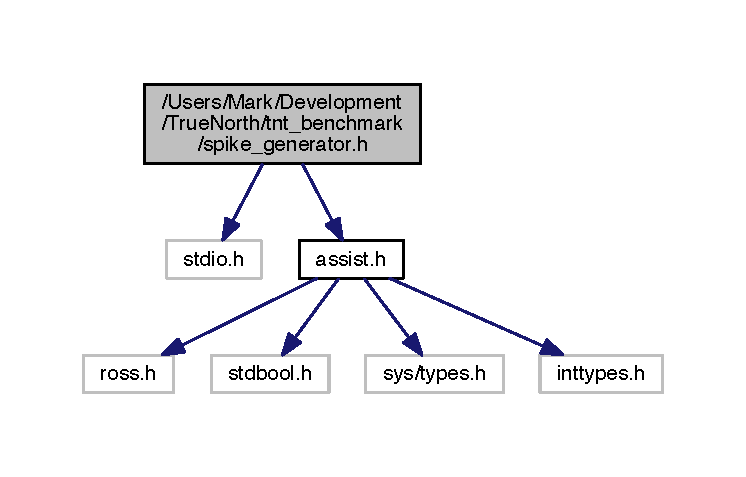
\includegraphics[width=350pt]{spike__generator_8h__incl}
\end{center}
\end{figure}
This graph shows which files directly or indirectly include this file\+:\nopagebreak
\begin{figure}[H]
\begin{center}
\leavevmode
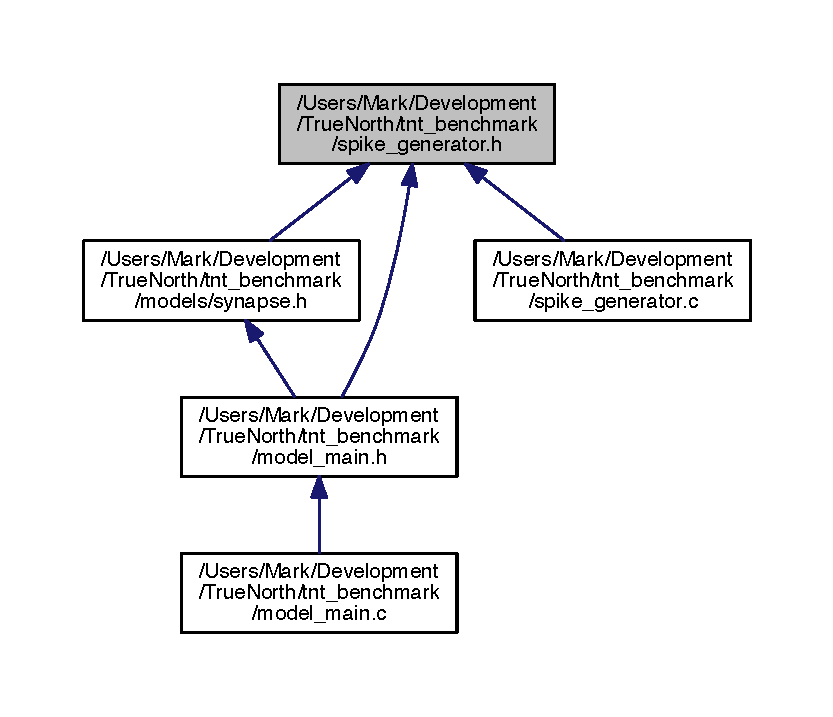
\includegraphics[width=350pt]{spike__generator_8h__dep__incl}
\end{center}
\end{figure}
\subsection*{Data Structures}
\begin{DoxyCompactItemize}
\item 
struct \hyperlink{structrandom_spikes}{random\+Spikes}
\begin{DoxyCompactList}\small\item\em Struct that genreates spikes randomly. \end{DoxyCompactList}\item 
struct \hyperlink{structselected_spikes}{selected\+Spikes}
\item 
struct \hyperlink{structspike_gen_state}{spike\+Gen\+State}
\begin{DoxyCompactList}\small\item\em Struct that manages the spike generator. \end{DoxyCompactList}\end{DoxyCompactItemize}
\subsection*{Typedefs}
\begin{DoxyCompactItemize}
\item 
typedef bool($\ast$ \hyperlink{spike__generator_8h_aa47e87d309aab7727810011578bae86e}{spike\+Gen\+Del}) (void $\ast$spike\+Gen, tw\+\_\+lp $\ast$lp)
\begin{DoxyCompactList}\small\item\em Spike\+Generator Function Pointer. \end{DoxyCompactList}\end{DoxyCompactItemize}
\subsection*{Enumerations}
\begin{DoxyCompactItemize}
\item 
enum \hyperlink{spike__generator_8h_ad05574e5624d82eeb7acf436ba8802f6}{random\+Select} \{ \\*
\hyperlink{spike__generator_8h_ad05574e5624d82eeb7acf436ba8802f6a4b3574e75cec43aa4dd3a0fd7940c632}{U\+N\+F}, 
\hyperlink{spike__generator_8h_ad05574e5624d82eeb7acf436ba8802f6a25f966031f3630b7ea2a347fa376b757}{E\+X\+P}, 
\hyperlink{spike__generator_8h_ad05574e5624d82eeb7acf436ba8802f6a0a5faa91345ab363e44d91656fbe435a}{B\+I\+N\+O\+M}, 
\hyperlink{spike__generator_8h_ad05574e5624d82eeb7acf436ba8802f6aa0e01bf1936fac473412454a1cf09569}{G\+E\+O\+M}, 
\\*
\hyperlink{spike__generator_8h_ad05574e5624d82eeb7acf436ba8802f6a1697a91b22c2369eb2ba427c2d193329}{S\+E\+L\+E\+C\+T}
 \}
\begin{DoxyCompactList}\small\item\em Enum that selects the type of random number generation. \end{DoxyCompactList}\end{DoxyCompactItemize}
\subsection*{Functions}
\begin{DoxyCompactItemize}
\item 
bool \hyperlink{spike__generator_8h_ac3b37f38c4efeef795767d85d9f85e46}{random\+Gen} (void $\ast$gen\+\_\+state, tw\+\_\+lp $\ast$lp)
\item 
bool \hyperlink{spike__generator_8h_ad6244e86a3542f8d3c64766e7e7c6746}{uniform\+Gen} (void $\ast$gen\+\_\+state, tw\+\_\+lp $\ast$lp)
\item 
bool \hyperlink{spike__generator_8h_a99c97d86709314338427c93f0e933667}{geometric\+Gen} (void $\ast$gen\+\_\+state, tw\+\_\+lp $\ast$lp)
\item 
bool \hyperlink{spike__generator_8h_a76ae6dc6c6885cf9652efb4947782351}{bin\+Gen} (void $\ast$gen\+\_\+state, tw\+\_\+lp $\ast$lp)
\item 
bool \hyperlink{spike__generator_8h_a7859f15c9115868c5c0ed88c43756482}{selected\+Gen} (void $\ast$spike\+Gen, tw\+\_\+lp $\ast$lp)
\end{DoxyCompactItemize}
\subsection*{Variables}
\begin{DoxyCompactItemize}
\item 
float \hyperlink{spike__generator_8h_a7d0ee5ac4ade99cd72e7b77bec9f8760}{rand\+Val}
\begin{DoxyCompactList}\small\item\em Selected random generator. \end{DoxyCompactList}\end{DoxyCompactItemize}


\subsection{Detailed Description}
spike\+\_\+generate defines a L\+P state and functions that generate output at a tuneable rate. 

Tool that generates spikes. Currently, a pseudo random input function is included. T\+N\+T\+\_\+\+M\+A\+I\+N Created by Mark Plagge on 4/14/15. \begin{DoxyAuthor}{Author}
Mark Plagge 
\end{DoxyAuthor}


\subsection{Typedef Documentation}
\hypertarget{spike__generator_8h_aa47e87d309aab7727810011578bae86e}{}\index{spike\+\_\+generator.\+h@{spike\+\_\+generator.\+h}!spike\+Gen\+Del@{spike\+Gen\+Del}}
\index{spike\+Gen\+Del@{spike\+Gen\+Del}!spike\+\_\+generator.\+h@{spike\+\_\+generator.\+h}}
\subsubsection[{spike\+Gen\+Del}]{\setlength{\rightskip}{0pt plus 5cm}typedef bool($\ast$ spike\+Gen\+Del) (void $\ast$spike\+Gen, tw\+\_\+lp $\ast$lp)}\label{spike__generator_8h_aa47e87d309aab7727810011578bae86e}


Spike\+Generator Function Pointer. 

Chooses the spike method function. 

Definition at line 26 of file spike\+\_\+generator.\+h.



\subsection{Enumeration Type Documentation}
\hypertarget{spike__generator_8h_ad05574e5624d82eeb7acf436ba8802f6}{}\index{spike\+\_\+generator.\+h@{spike\+\_\+generator.\+h}!random\+Select@{random\+Select}}
\index{random\+Select@{random\+Select}!spike\+\_\+generator.\+h@{spike\+\_\+generator.\+h}}
\subsubsection[{random\+Select}]{\setlength{\rightskip}{0pt plus 5cm}enum {\bf random\+Select}}\label{spike__generator_8h_ad05574e5624d82eeb7acf436ba8802f6}


Enum that selects the type of random number generation. 

\begin{Desc}
\item[Enumerator]\par
\begin{description}
\index{U\+N\+F@{U\+N\+F}!spike\+\_\+generator.\+h@{spike\+\_\+generator.\+h}}\index{spike\+\_\+generator.\+h@{spike\+\_\+generator.\+h}!U\+N\+F@{U\+N\+F}}\item[{\em 
\hypertarget{spike__generator_8h_ad05574e5624d82eeb7acf436ba8802f6a4b3574e75cec43aa4dd3a0fd7940c632}{}U\+N\+F\label{spike__generator_8h_ad05574e5624d82eeb7acf436ba8802f6a4b3574e75cec43aa4dd3a0fd7940c632}
}]\index{E\+X\+P@{E\+X\+P}!spike\+\_\+generator.\+h@{spike\+\_\+generator.\+h}}\index{spike\+\_\+generator.\+h@{spike\+\_\+generator.\+h}!E\+X\+P@{E\+X\+P}}\item[{\em 
\hypertarget{spike__generator_8h_ad05574e5624d82eeb7acf436ba8802f6a25f966031f3630b7ea2a347fa376b757}{}E\+X\+P\label{spike__generator_8h_ad05574e5624d82eeb7acf436ba8802f6a25f966031f3630b7ea2a347fa376b757}
}]\index{B\+I\+N\+O\+M@{B\+I\+N\+O\+M}!spike\+\_\+generator.\+h@{spike\+\_\+generator.\+h}}\index{spike\+\_\+generator.\+h@{spike\+\_\+generator.\+h}!B\+I\+N\+O\+M@{B\+I\+N\+O\+M}}\item[{\em 
\hypertarget{spike__generator_8h_ad05574e5624d82eeb7acf436ba8802f6a0a5faa91345ab363e44d91656fbe435a}{}B\+I\+N\+O\+M\label{spike__generator_8h_ad05574e5624d82eeb7acf436ba8802f6a0a5faa91345ab363e44d91656fbe435a}
}]\index{G\+E\+O\+M@{G\+E\+O\+M}!spike\+\_\+generator.\+h@{spike\+\_\+generator.\+h}}\index{spike\+\_\+generator.\+h@{spike\+\_\+generator.\+h}!G\+E\+O\+M@{G\+E\+O\+M}}\item[{\em 
\hypertarget{spike__generator_8h_ad05574e5624d82eeb7acf436ba8802f6aa0e01bf1936fac473412454a1cf09569}{}G\+E\+O\+M\label{spike__generator_8h_ad05574e5624d82eeb7acf436ba8802f6aa0e01bf1936fac473412454a1cf09569}
}]\index{S\+E\+L\+E\+C\+T@{S\+E\+L\+E\+C\+T}!spike\+\_\+generator.\+h@{spike\+\_\+generator.\+h}}\index{spike\+\_\+generator.\+h@{spike\+\_\+generator.\+h}!S\+E\+L\+E\+C\+T@{S\+E\+L\+E\+C\+T}}\item[{\em 
\hypertarget{spike__generator_8h_ad05574e5624d82eeb7acf436ba8802f6a1697a91b22c2369eb2ba427c2d193329}{}S\+E\+L\+E\+C\+T\label{spike__generator_8h_ad05574e5624d82eeb7acf436ba8802f6a1697a91b22c2369eb2ba427c2d193329}
}]\end{description}
\end{Desc}


Definition at line 16 of file spike\+\_\+generator.\+h.


\begin{DoxyCode}
16                           \{
17     \hyperlink{spike__generator_8h_ad05574e5624d82eeb7acf436ba8802f6a4b3574e75cec43aa4dd3a0fd7940c632}{UNF},
18     \hyperlink{spike__generator_8h_ad05574e5624d82eeb7acf436ba8802f6a25f966031f3630b7ea2a347fa376b757}{EXP},
19     \hyperlink{spike__generator_8h_ad05574e5624d82eeb7acf436ba8802f6a0a5faa91345ab363e44d91656fbe435a}{BINOM},
20     \hyperlink{spike__generator_8h_ad05574e5624d82eeb7acf436ba8802f6aa0e01bf1936fac473412454a1cf09569}{GEOM},
21     \hyperlink{spike__generator_8h_ad05574e5624d82eeb7acf436ba8802f6a1697a91b22c2369eb2ba427c2d193329}{SELECT}
22 \}\hyperlink{spike__generator_8h_ad05574e5624d82eeb7acf436ba8802f6}{randomSelect};
\end{DoxyCode}


\subsection{Function Documentation}
\hypertarget{spike__generator_8h_a76ae6dc6c6885cf9652efb4947782351}{}\index{spike\+\_\+generator.\+h@{spike\+\_\+generator.\+h}!bin\+Gen@{bin\+Gen}}
\index{bin\+Gen@{bin\+Gen}!spike\+\_\+generator.\+h@{spike\+\_\+generator.\+h}}
\subsubsection[{bin\+Gen}]{\setlength{\rightskip}{0pt plus 5cm}bool bin\+Gen (
\begin{DoxyParamCaption}
\item[{void $\ast$}]{gen\+\_\+state, }
\item[{tw\+\_\+lp $\ast$}]{lp}
\end{DoxyParamCaption}
)}\label{spike__generator_8h_a76ae6dc6c6885cf9652efb4947782351}
\hypertarget{spike__generator_8h_a99c97d86709314338427c93f0e933667}{}\index{spike\+\_\+generator.\+h@{spike\+\_\+generator.\+h}!geometric\+Gen@{geometric\+Gen}}
\index{geometric\+Gen@{geometric\+Gen}!spike\+\_\+generator.\+h@{spike\+\_\+generator.\+h}}
\subsubsection[{geometric\+Gen}]{\setlength{\rightskip}{0pt plus 5cm}bool geometric\+Gen (
\begin{DoxyParamCaption}
\item[{void $\ast$}]{gen\+\_\+state, }
\item[{tw\+\_\+lp $\ast$}]{lp}
\end{DoxyParamCaption}
)}\label{spike__generator_8h_a99c97d86709314338427c93f0e933667}
\hypertarget{spike__generator_8h_ac3b37f38c4efeef795767d85d9f85e46}{}\index{spike\+\_\+generator.\+h@{spike\+\_\+generator.\+h}!random\+Gen@{random\+Gen}}
\index{random\+Gen@{random\+Gen}!spike\+\_\+generator.\+h@{spike\+\_\+generator.\+h}}
\subsubsection[{random\+Gen}]{\setlength{\rightskip}{0pt plus 5cm}bool random\+Gen (
\begin{DoxyParamCaption}
\item[{void $\ast$}]{gen\+\_\+state, }
\item[{tw\+\_\+lp $\ast$}]{lp}
\end{DoxyParamCaption}
)}\label{spike__generator_8h_ac3b37f38c4efeef795767d85d9f85e46}
\hypertarget{spike__generator_8h_a7859f15c9115868c5c0ed88c43756482}{}\index{spike\+\_\+generator.\+h@{spike\+\_\+generator.\+h}!selected\+Gen@{selected\+Gen}}
\index{selected\+Gen@{selected\+Gen}!spike\+\_\+generator.\+h@{spike\+\_\+generator.\+h}}
\subsubsection[{selected\+Gen}]{\setlength{\rightskip}{0pt plus 5cm}bool selected\+Gen (
\begin{DoxyParamCaption}
\item[{void $\ast$}]{spike\+Gen, }
\item[{tw\+\_\+lp $\ast$}]{lp}
\end{DoxyParamCaption}
)}\label{spike__generator_8h_a7859f15c9115868c5c0ed88c43756482}
\hypertarget{spike__generator_8h_ad6244e86a3542f8d3c64766e7e7c6746}{}\index{spike\+\_\+generator.\+h@{spike\+\_\+generator.\+h}!uniform\+Gen@{uniform\+Gen}}
\index{uniform\+Gen@{uniform\+Gen}!spike\+\_\+generator.\+h@{spike\+\_\+generator.\+h}}
\subsubsection[{uniform\+Gen}]{\setlength{\rightskip}{0pt plus 5cm}bool uniform\+Gen (
\begin{DoxyParamCaption}
\item[{void $\ast$}]{gen\+\_\+state, }
\item[{tw\+\_\+lp $\ast$}]{lp}
\end{DoxyParamCaption}
)}\label{spike__generator_8h_ad6244e86a3542f8d3c64766e7e7c6746}


Definition at line 11 of file spike\+\_\+generator.\+c.


\begin{DoxyCode}
11                                            \{
12     \textcolor{keywordtype}{bool} willFire = \textcolor{keyword}{false};
13     
14     \hyperlink{structspike_gen_state}{spikeGenState} * st = (\hyperlink{structspike_gen_state}{spikeGenState} * ) spikeGen;
15     tw\_rng\_stream *str = (tw\_rng\_stream *) lp->rng;
16         \textcolor{keywordflow}{if}(tw\_rand\_unif(str) < st->\hyperlink{structspike_gen_state_a57768e1ceaa4dd88752232ad89b4e8b7}{rndSpikes}.\hyperlink{structrandom_spikes_a1333eb5695ae83d1ffccf24b08bc6288}{randomRate} / 100 )
17         willFire = \textcolor{keyword}{true};
18     \textcolor{keywordflow}{return} willFire;
19 \}
\end{DoxyCode}


\subsection{Variable Documentation}
\hypertarget{spike__generator_8h_a7d0ee5ac4ade99cd72e7b77bec9f8760}{}\index{spike\+\_\+generator.\+h@{spike\+\_\+generator.\+h}!rand\+Val@{rand\+Val}}
\index{rand\+Val@{rand\+Val}!spike\+\_\+generator.\+h@{spike\+\_\+generator.\+h}}
\subsubsection[{rand\+Val}]{\setlength{\rightskip}{0pt plus 5cm}float rand\+Val}\label{spike__generator_8h_a7d0ee5ac4ade99cd72e7b77bec9f8760}


Selected random generator. 



Definition at line 32 of file spike\+\_\+generator.\+h.


%--- End generated contents ---

% Bibliography
\newpage
\phantomsection
\bibliographystyle{plain}
\bibliography{}
\addcontentsline{toc}{chapter}{Bibliography}

% Index
\backmatter
\newpage
\phantomsection
\clearemptydoublepage
\addcontentsline{toc}{chapter}{Index}
\printindex

\end{document}
